\documentclass[12pt,a4]{article}
\usepackage[a4paper, total={6.5in, 8.5in}]{geometry}
\usepackage{moreverb,url}
\usepackage[colorlinks,bookmarksopen,bookmarksnumbered,citecolor=red,urlcolor=red]{hyperref}
\usepackage{amssymb}
\usepackage{graphicx}
\usepackage[utf8]{inputenc}
\usepackage{amsmath}
\usepackage{pdfpages}
\usepackage{epstopdf}
\usepackage[english]{babel}
\usepackage{mathrsfs}
\usepackage{hyperref}
\usepackage{caption}
\usepackage{color}
\usepackage{float}
\usepackage[noabbrev]{cleveref}
\crefname{appsec}{appendix}{appendices}
\crefname{algocf}{algorithm}{algorithms}
\Crefname{algocf}{Algorithm}{Algorithms}
\usepackage{subcaption}
\usepackage{algorithm2e,algorithmic}
\usepackage{appendix}
%\usepackage{breqn}
\DeclareMathOperator{\sech}{sech}
\DeclareMathOperator*{\argmin}{arg\,min}

%
\bibliographystyle{elsarticle-num}

\begin{document}
%
\title{Motion planning of hyper-redundant robot through confined paths}
%
%
\author{K. P. Ashwin*, Arkadeep N. C.
\thanks{Graduate Student at the Robotics and Design Lab, Department
of Mechanical Engineering, Indian Institute of Science, Bangalore 560012, India, email: ashwinkp@iisc.ac.in}, 
 and A. Ghosal
\thanks{Corresponding Author, Professor, Department of Mechanical Engineering, Indian Institute of Science, Bangalore, email: asitava@iisc.ac.in.}}
%
%double spacing for submission
%\baselineskip 12pt plus 0.5pt minus 0.5pt 
\baselineskip 18pt plus 0.5pt minus 0.5pt
%
\date{}
\maketitle
\begin{abstract}
\label{sec:abstract}

Application of highly articulated hyper-redundant robots to manoeuvre in narrow and confined spaces is gaining popularity due to their obvious advantages. Given a path which the end-effector has to traverse, finding the configuration which avoids collision with the environment constitutes obstacle-avoided redundancy resolution and subsequently, the motion planning of the robot. While there are many redundancy resolution methods which address obstacle avoidance, tractrix based optimization method produces displacement of links which attenuates from the end-effector tip to the base of the robot and thereby simulating a more `natural' motion. While tractrix based methods are studied for obstacle avoidance, application of the method for robots confined within a narrow bounded path(duct) is not very well studied. This paper presents different ways in which ducts can be modelled in 2D plane as well as in 3D space and how motion planning can be achieved using tractrix based methods in each cases. Fundamental formulations and well as more efficient formulations for practical implementation have been discussed. The concepts are demonstrated using simulations conducted on three practical scenarios: 1) hyper-redundant manipulators inspecting an industrial pipeline, 2) motion of an endoscopic robot through GI tract and 3) motion of hyper-redundant manipulators in search and rescue operations. Analysis on the computational complexity shows that the method is feasible for practical implementation. 

\end{abstract}

\textbf{Keywords}:6 keywords
%\linenumbers

\section{Introduction}
\label{sec:introduction}

In the reachable workspace of a serial robot in 3D, since a given position and orientation of end-effector can be achieved using a maximum of six joints, additional joints would create a redundant system. Such robots are generally termed redundant serial robots. While robots with 6 joints  or less can achieve a position and orientation in space with limited configurations, there are theoretically infinite possibilities for a hyper-redundant robot to achieve the same. These additional degrees of freedom can be effectively used in situations where the robot has to selectively choose configurations without altering the end-effector pose, such as robotic manipulation through confined spaces. This renders the potential use of highly articulated hyper-redundant robots in applications such as exploring earthquake hit regions for search and rescue operations [ref Wolf 2003, Murphy 2008], remotely operated robotic arms for minimally invasive laparoscopic and endoscopic surgeries [ref Slatkin 1995 Howe 1999 Cadiere2001 Murphy2008 Burgner-Kahrs2015] and inspection of industrial pipelines and nuclear reactors[ref Paljug1995 Chirikjian1991 William 1997 Gargiulo2009 Ma1994]. A large number of redundant joints also make the robots analogous in morphology to  snake, elephant trunk, tentacle etc. and hence, a topic of particular interest in bio-inspired robotics [ref Hirose2004 Hannan2000 Chirikjian1993]. Identifying a suitable configuration from the many possible configurations, given the position and orientation of the end-effector constitutes the redundancy resolution of hyper-redundant robots. If the path through which the end-effector has to follow is predetermined, then the redundancy resolution problem also constitutes the motion planning of the robot.

The initial focus of researchers on addressing redundancy resolution problem was to solve the equation $\dot{\mathbf{\vartheta}}=J\left(\mathbf{\varphi} \right)\dot{\mathbf{\varphi}}$ where $J$ is the manipulator Jacobian matrix and $\vartheta$ and $\varphi$ are the vectors in task space and joint space respectively. Primary idea of inverse kinematics is to invert the Jacobian using Moore-Penrose inverse(pseudo inverse). While this method results in kinematic singularities, methods such as extended Jacobian[ ref Leigois1977, JohnBaillieul1984 ] and task prioritized augmented Jacobian[ ref Maciejewski1985] are aimed to avoid these singularities and also obtain solutions to inverse kinematic problem by specifying a velocity component at the singular configuration depending on the task at hand. Since the major advantage of using a hyper-redundant robot is to facilitate motion avoiding obstacles and movement in confined spaces, many researchers have worked on this particular task using above mentioned techniques [ref Hwang1992]. However, even though the methods avoid singularities in the manipulator Jacobian, it could generate other forms of singularities and also, the method becomes computationally complex for large number of joints [ref Chiaverini1997]. Many other redundancy resolution methods including variational approach, geometric approach, neural networks and fuzzy logic can also be found in the literature. [ref Sciavicco1988, Mao1997, Dasgupta, Antonelli2003]. In [ref Chirikjian1991], obstacle avoidance problem for hyper-redundant manipulator is carried out by fitting a curve through the joints of manipulator and planning the path for this `backbone curve' which avoids obstacles. Finding the pose of the backbone curve directly gives the co-ordinates of the joints. Hence, in case of obstacle cluttered environments, planning the path of the end-effector which avoids the obstacles will result in redundancy resolution since the trajectory itself forms the backbone curve of the manipulator[ref Latombe1991, Khatib1986, Lumelsky1987, Choset2001]. 

Even though the backbone curve approach is very simple, end-effector trajectory with many kinks may sometimes produce undesirably high acceleration at the tail of the link as shown in \cref{fig:backbone}. The motion will also look un-natural. In [ref], the authors proposed a tractrix based redundancy resolving algorithm which produces natural looking motion of hyper-redundant robot. It is also shown in [ref] that the same can be achieved by minimizing the subsequent motion of the links, given the displacement of the head(end-effector), and the motion attenuates from the head to the tail(base) of the entire manipulator. For obstacles represented by simple analytical shapes, the algorithm can be effectively used for obstacle avoidance of the entire link chain as well[ref]. However, in the special case of motion through confined spaces within a narrow bounded path (which hereafter we call ``duct''), directly implementing the algorithm would require modeling the entire half space outside the duct as obstacles which is impractical. In this paper, we discuss a few methods to represent ducts and how to implement tractrix-based algorithm for motion planning of a hyper-redundant robot. In section \ref{sec:Tractrixoverview}, an overview of tractrix based algorithm and the physical tractability of the algorithm is discussed. Representation of ducts in 2D plane and motion planning through the planar ducts is detailed in section \ref{sec:2Dmotionplanning}. Representation of ducts in 3D and motion planning in the same is explained in \cref{sec:3Dmotionplanning}. In section \ref{sec:Examples}, we demonstrate the concepts by simulating the motion of hyper-redundant robots in three practical applications. Advantage of this method in terms of computational complexity and the limitations of this method is also mentioned in the section. Finally, in section \ref{sec:conclusions}, we present the conclusions of the paper and the scope of future work.

\begin{figure}[ht!]
    \centering
    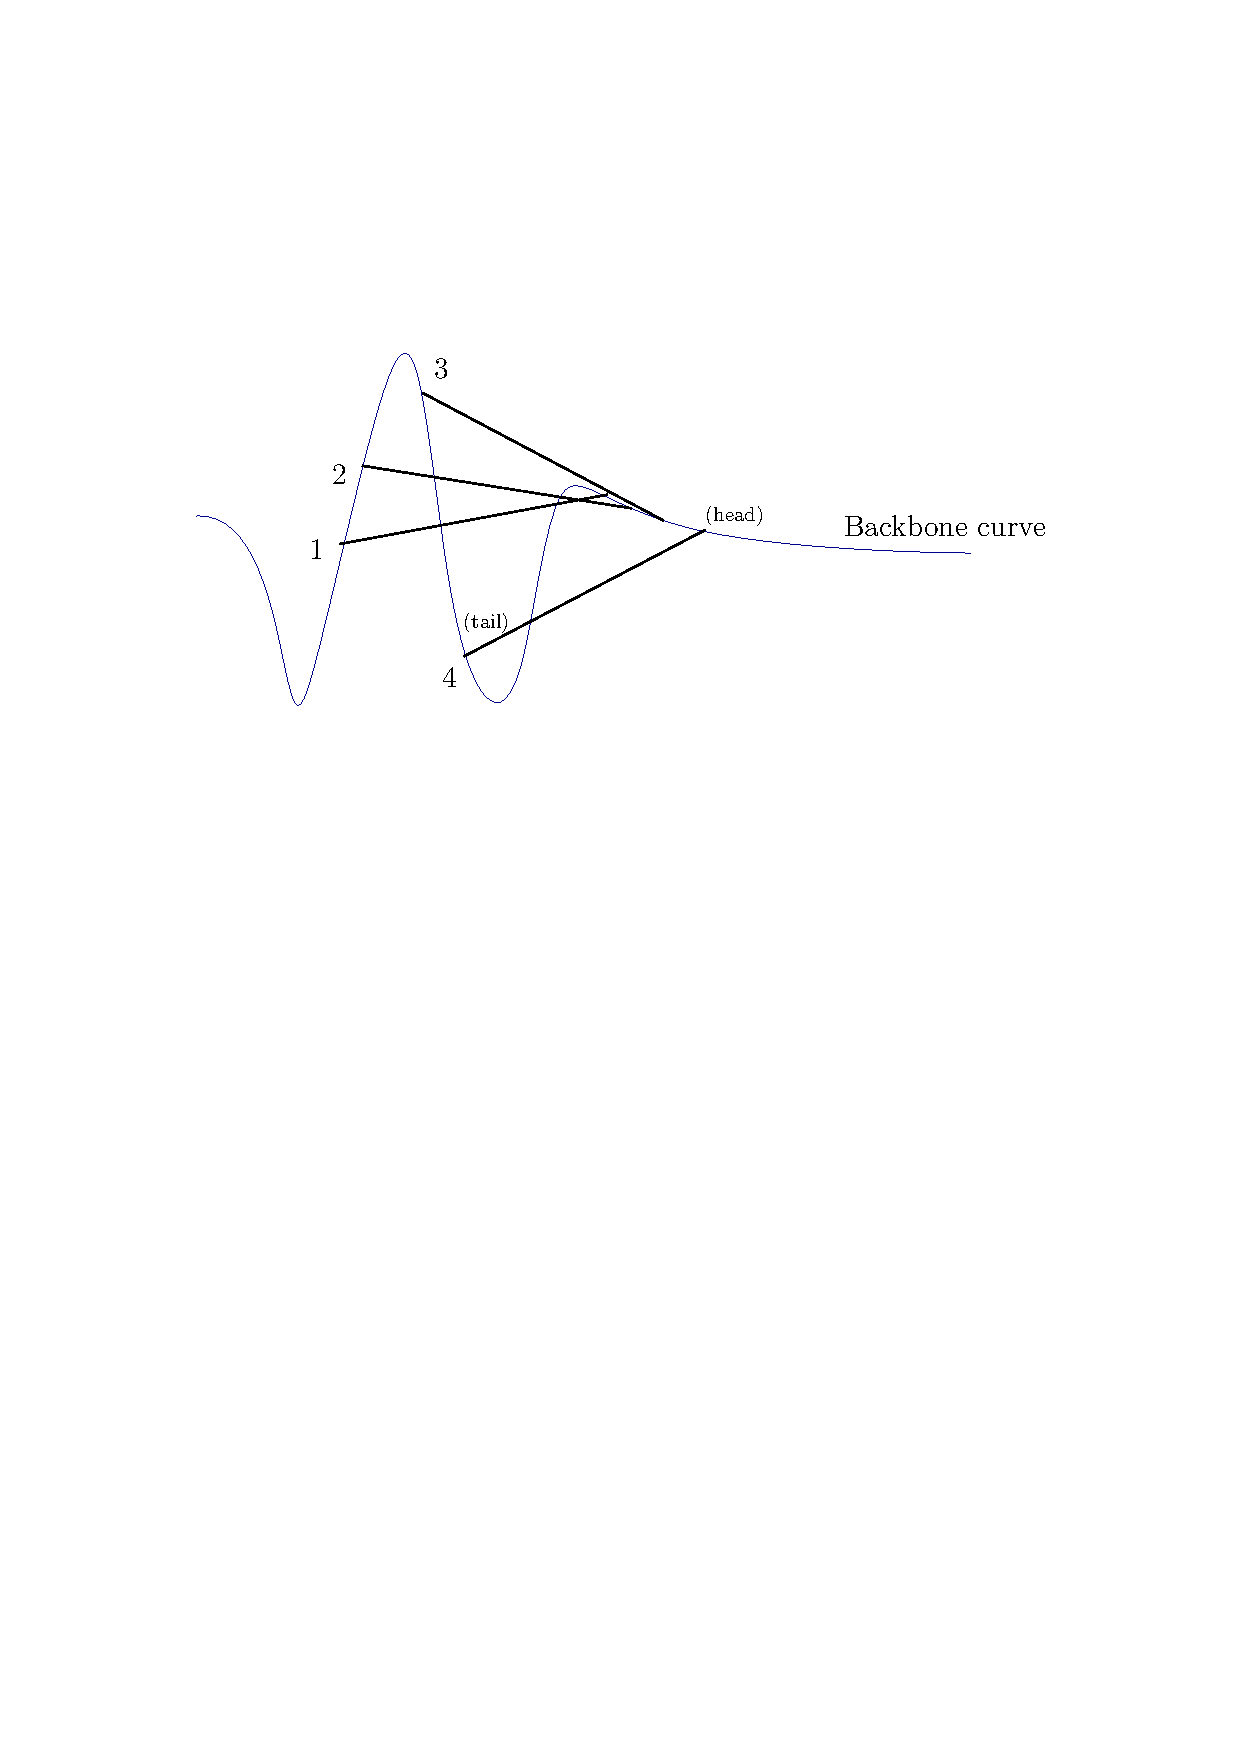
\includegraphics[scale=0.75]{figures/backbone.pdf}
        \caption{Large motion in tail corresponding to small head movement for single link}
        \label{fig:backbone}
\end{figure}

\section{Overview of tractrix based motion planning}
\label{sec:Tractrixoverview}
%
Consider a rigid link of length $L_0$ positioned in a 2D plane, initially aligned to the Y-axis as shown in \cref{fig:tractrixin2D} . The co-ordinates of the `head' of the link is given as $\textbf{X}_h = [X_h,Y_h]^T$ and the co-ordinates of the `tail' as $\textbf{X}_t = [X_t,Y_t]^T$. If the head is displaced to the co-ordinate $\textbf{x}_h = [x_h,y_h]$ along the positive $X-$ axis by $t$ units, the tail of the link can lie anywhere on the circumference of a circle centered at the co-ordinate $(t,0)$ with radius $L_0$. If we assign a rule that the velocity of the tail of the link is always directed towards the length of the link, we get two diametrically opposite points on the circle. The continuous path traced by the tail point is the well known tractrix curve as given in \cref{eq:tractrix}:
\begin{align}
\label{eq:tractrix}
\textbf{x}_t = [x(t),y(t)] = [t-L_0\tanh\frac{t}{L_0},L_0\sech\frac{t}{L_0}]
\end{align}
The extension of tractrix equation along motion in arbitrary direction as well as an algorithm to calculate the same in 3-D can be found in [ref] and [ref]. In case of multiple links connected to each other as in the case of a hyper-redundant robot, or a one dimensional object approximated as a series of connected linkages, the algorithm can be applied iteratively from the head to tail as shown in [ref]. By moving along the tractix curve, the tail moves the minimum distance with respect to its initial position. Also, the displacement $\Vert \textbf{x}_h-\textbf{X}_h \Vert \geq \Vert \textbf{x}_t-\textbf{X}_t \Vert$ which means that the displacement attentuates from the displaced link to end of the chain in case of serially connected links as shown in \cref{fig:attenuation_of Motion}. Due to the minimal displacement of the tail, the motion can be imagined as the one with high lateral resistance on the link and less resistance in the direction of motion of link. 

\begin{figure}[ht!]
    \centering
    \begin{subfigure}{0.48\textwidth}
        \centering
        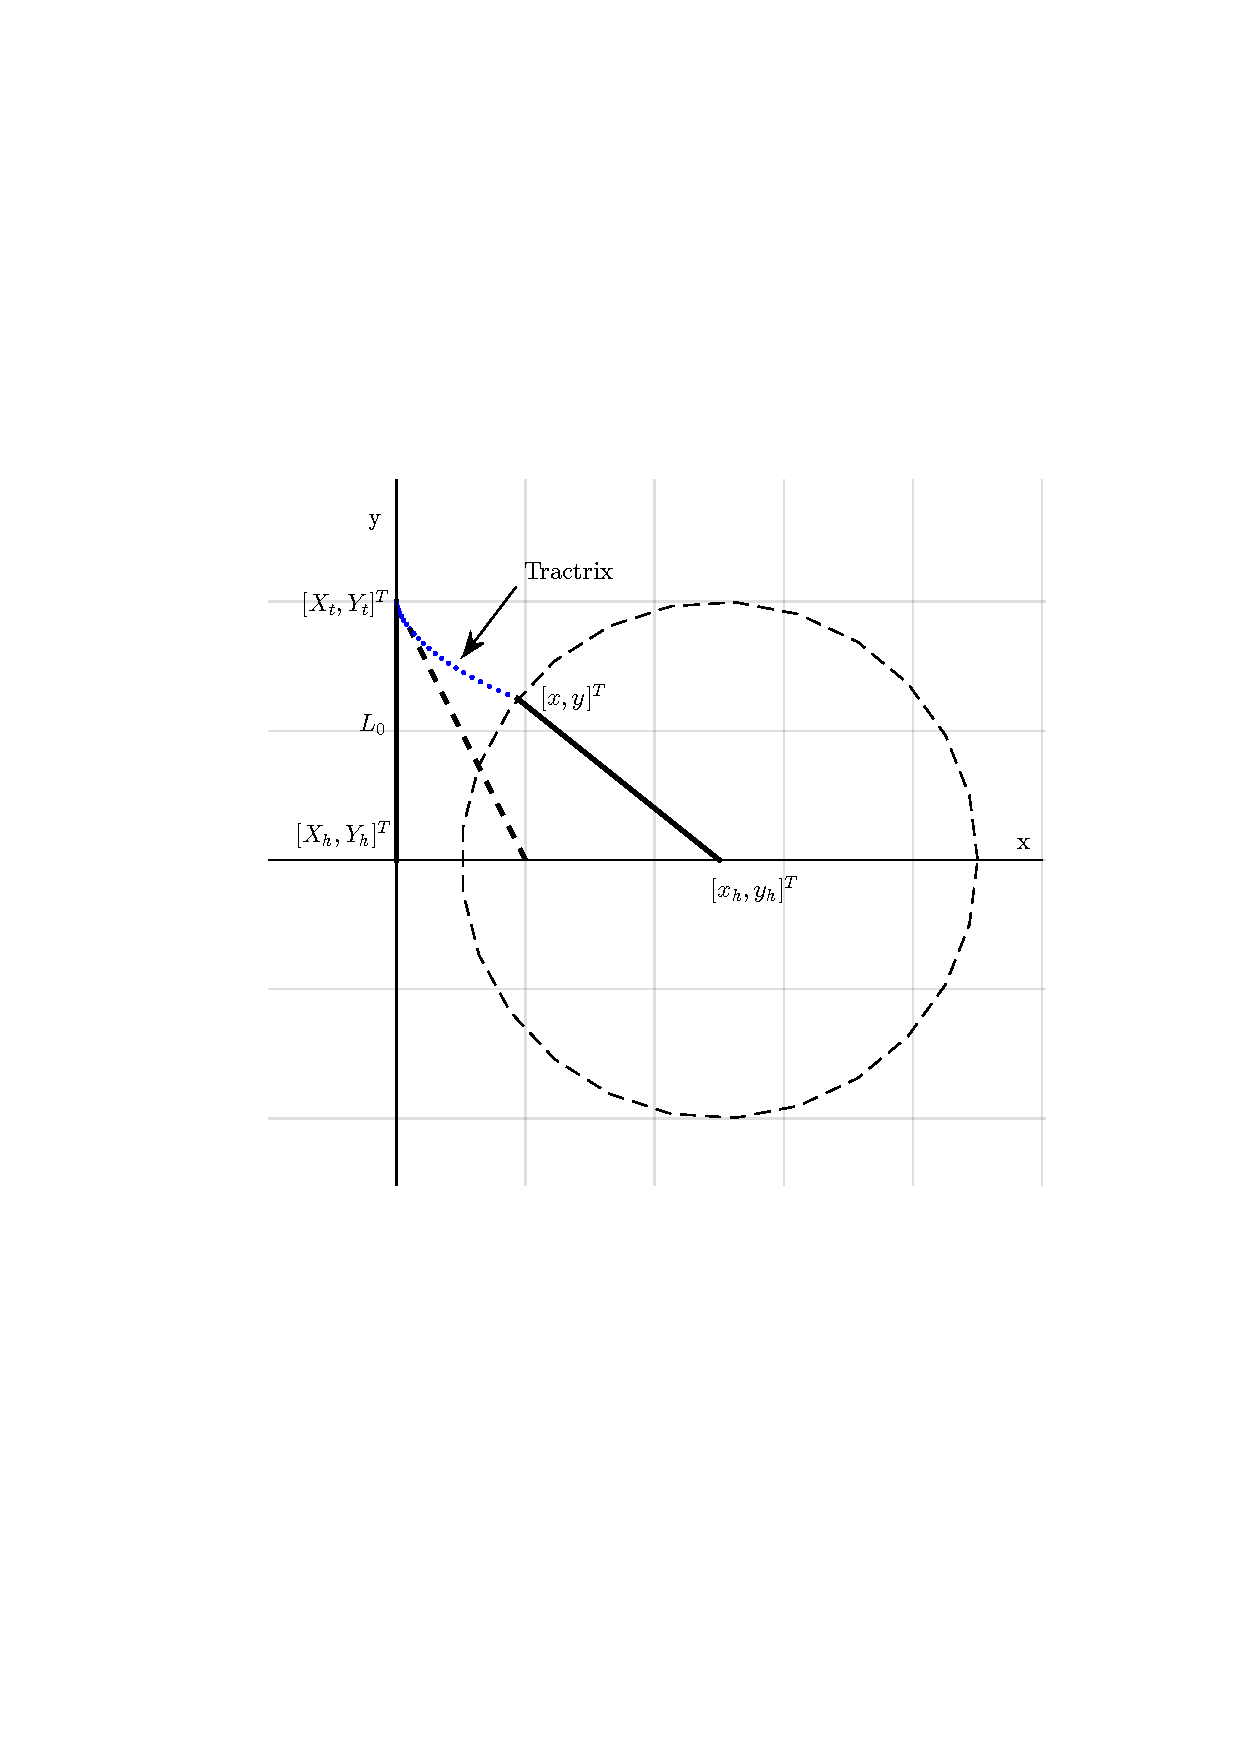
\includegraphics[width=\linewidth]{figures/fig1.pdf}
        \caption{Tractrix curve in 2D with one link}
        \label{fig:tractrixin2D}
    \end{subfigure}%
    \begin{subfigure}{0.48\textwidth}
        \centering
        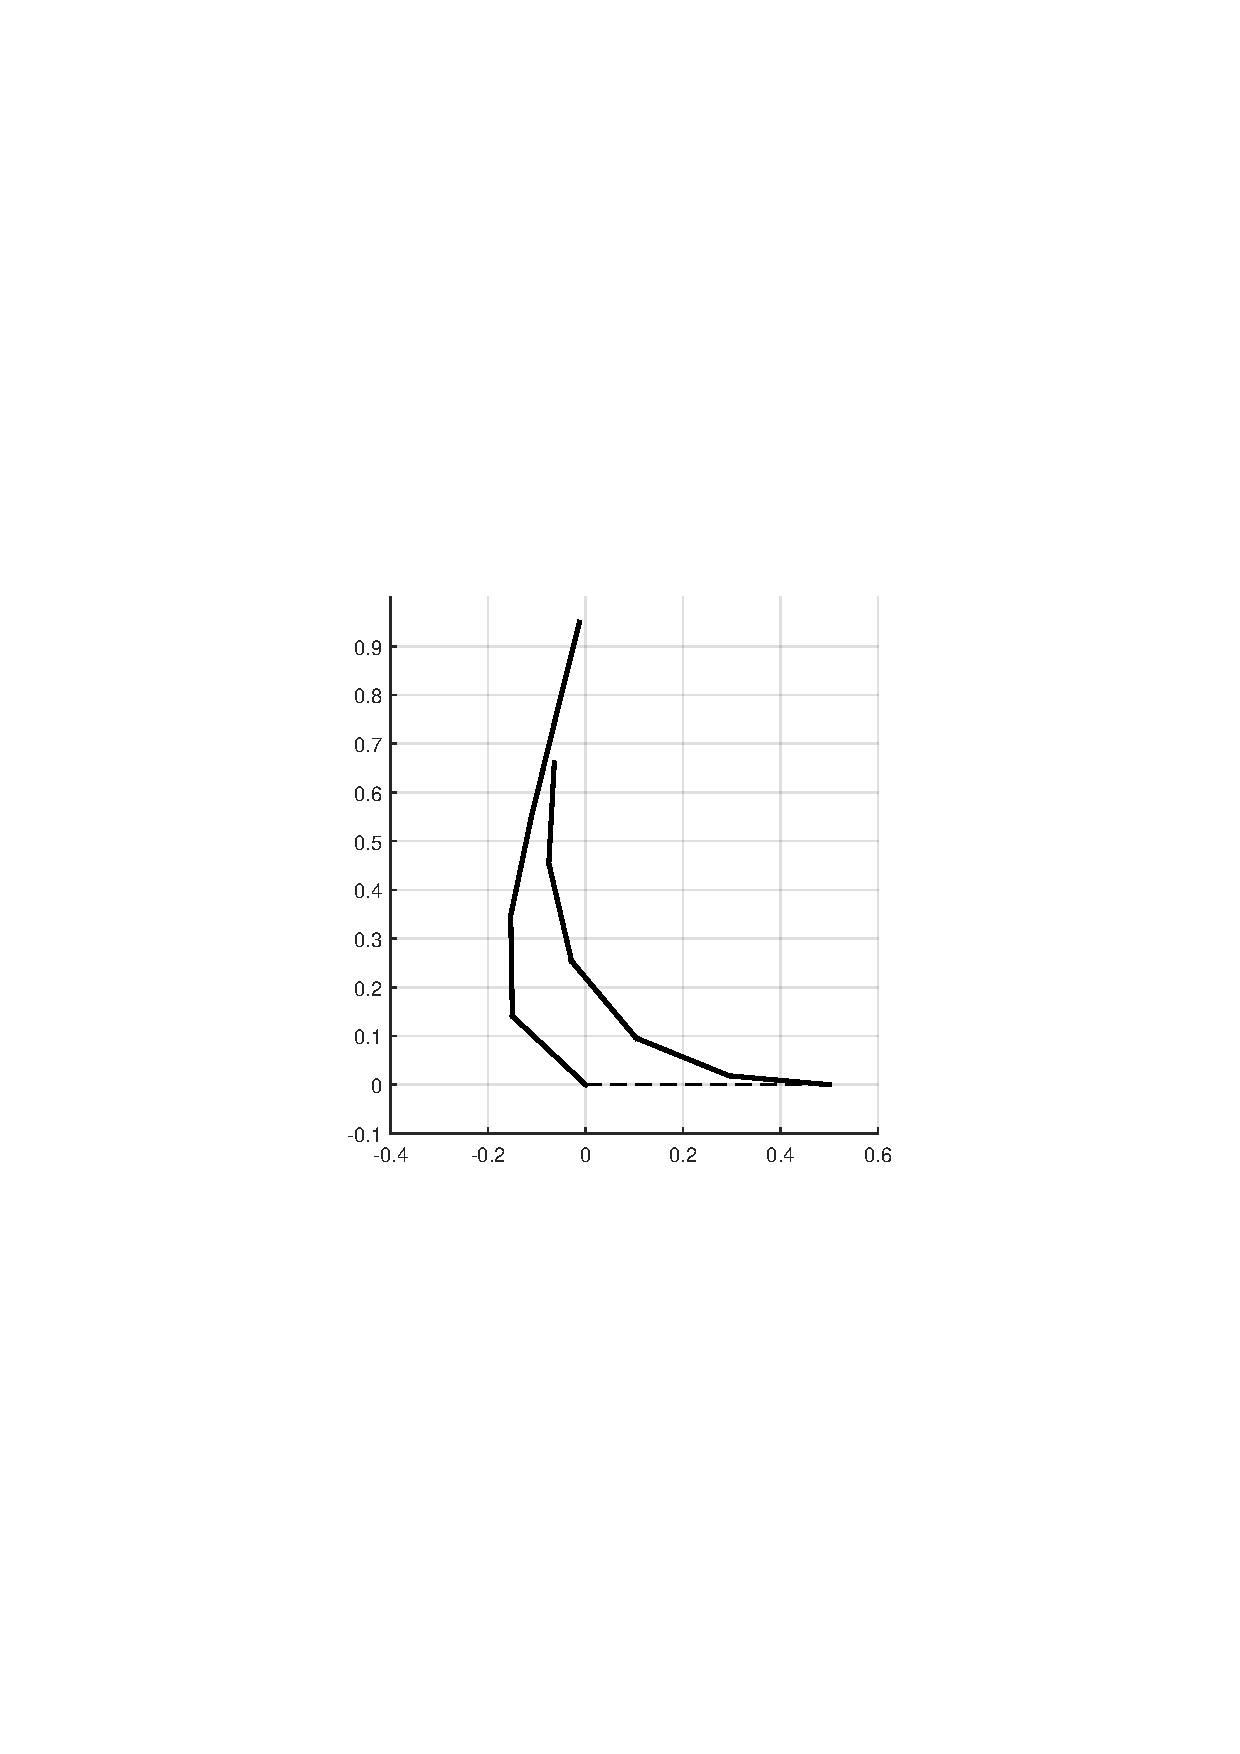
\includegraphics[width=0.75\linewidth]{figures/fig2.pdf}
        \caption{Tractrix with multiple links}
        \label{fig:attenuation_of Motion}
    \end{subfigure}
\caption{Tractrix in a plane}
\end{figure}


It is shown in [ref] that for a single rigid link, tractrix curve can also be obtained by minimizing an $L^2$ metric which is essentially the displacement of the tail from its initial position subject to the condition that the length of link is always preserved. i.e, the co-ordinates of the tail can be obtained from the following minimization problem:
\begin{align} \label{eq:Opt_prob_main}
\argmin_{\textbf{x}_t} &\Vert \textbf{x}_t-\textbf{X}_t \Vert\\
\text{Subject~ to:  } &\Vert \textbf{x}_h - \textbf{x}_t \Vert -L_0 = 0 \nonumber
\end{align}
An advantage of expressing tractrix as a minimization problem is that we can add more constraints to the above expression and hence, control the position of the tail point. Though the resulting curve may not necessarily be a tractix curve, the motion of the tail will appear realistic [ref]. For the motion of a link which minimizes its tail velocity (displacement of the tail co-ordinates), obstacle avoidance is achieved by formulating the problem as:
\begin{align} \label{eq:obstacle_avoidance_opt}
\argmin_{\textbf{x}_t} &\Vert \textbf{x}_t-\textbf{X}_t \Vert\\
\text{Subject to:} 
&\Vert \textbf{x}_h - \textbf{x}_t \Vert -L_0 = 0 \nonumber \\ 
~~ &f(\textbf{x}) \succeq 0  \nonumber
\end{align}
where $\bf{f}(x) = 0$ are the analytical equations of the boundaries of the surfaces which are to be avoided. For example, if the tail is to avoid a single obstacle represented by a circle with center $(x_c,y_c)$, the expression $f(x) = (x-x_c)^2+(y-y_c)^2-r^2>0$ ensures that the point $x$ always lies outside the circle of radius $r$. Complex objects can be modelled as a combination of super-ellipses as shown in [ref]. In this case, $\textbf{f}(x)$ will be a vector of all boundary equations $\textbf{f}(x) = [f_1(x),f_2(x),...f_m(x)]^T$. It is also worth noting that the value of constraint function in \cref{eq:obstacle_avoidance_opt} will increase or decrease as the point is farther from the curve $\textbf{f}(x)$; the value being zero on the curve. Hence, this approach can also be imagined as a geometric potential field, with zero potential only at the surface of the obstacle. 

\begin{figure}[h!]
\centering
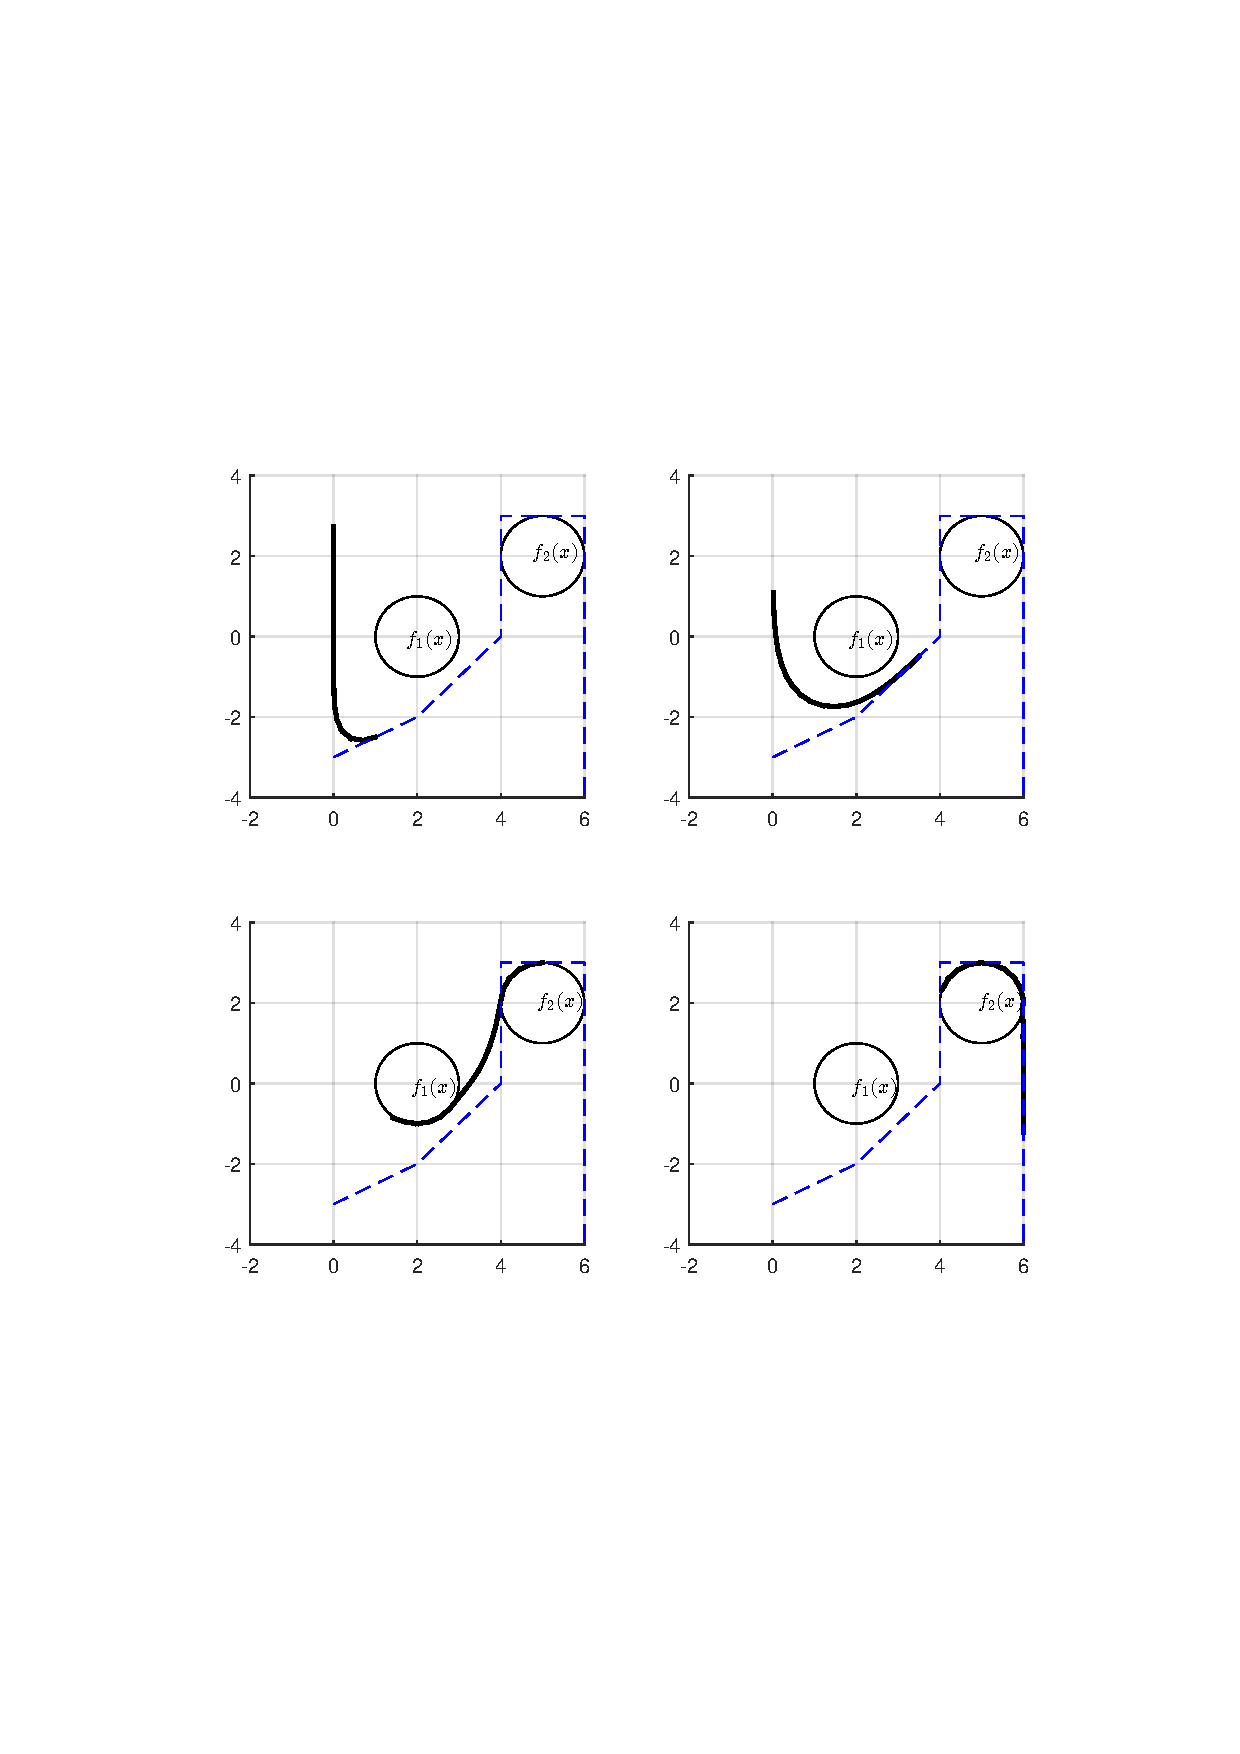
\includegraphics[scale=0.75]{figures/fig3.pdf}
\caption{Obstacle avoidance in a plane\label{fig:obstacle_avoidance_2D}}
\end{figure}

%In the case of motion planning of hyper-redundant manipulator, a quite a few problems deal with simulating the motion of the robot while traversing through a confined space within a narrow bounded path, which we term as a ``\textit{duct}" for the remainder of the paper. 
The problem of planning the motion of the robot through a duct may be specified as:
\begin{align} \label{eq:path_planning_opt}
\argmin_{\textbf{x}_t} &\Vert \textbf{x}_t-\textbf{X}_t \Vert\\
\text{Subject to:} &\Vert \textbf{x}_h - \textbf{x}_t \Vert -L_0 = 0 \nonumber \\
C_{\text{ineq}}:~~&{f}(x) < 0 \nonumber
\end{align}
While this expression is applicable for a duct represented by a single surface with the boundary $f(x)$, unlike the obstacle avoidance problem, the same will not work in the case of complex surfaces represented by combination of simpler analytical shapes. This is because if a point is classified as inside one of the simpler shapes, then it should be classified as outside the other shapes forming the duct. In other words, if one constraint function $f_k(x)< 0$, then the other constraint functions $f_{i\neq k}\geq 0$. In the next sections, we present different methods to represent the ducts and how confined space motion is achieved in different cases. 


\subsection{Nature of the optimization problem}\label{sc:optimization}
In the previous section we have discussed how tractrix based motion planning can be formulated as a constrained optimization problem, which entails a discussion on the suitability of the posed optimization problem and guarantee that the solution is unique and physically tractable. To address this, we will prove that the problem in \cref{eq:path_planning_opt} and the variations of the same used in the current work can be posed as convex problems. A function $f:\mathbb{R}^n\to \mathbb{R}$ is \textit{convex} if and only if the following two conditions hold:
\begin{enumerate}
	\item [a] The domain of $f$, $\textbf{dom}f$ is a convex set, and,
	\item [b]  For all $x,y \in \textbf{dom}f$ and $\theta$ with $0\leq \theta \leq 1$ \begin{equation}\label{eq:convex_fn}
	f(\theta x+(1-\theta)y)\leq \theta f(x)+(1-\theta)f(y)
	\end{equation}
\end{enumerate}
In our problem, the function is the $L_2$ norm of a vector in $\mathbb{R}^2$ or $\mathbb{R}^3$.  Though the $L_2$ norm is defined for all real vectors, the constraints ensuring that the object moves within the confinement of the duct restricts the domain to a feasible closed set $\mathcal{S}$\footnote{Assuming $\mathcal{S}$ to be a closed set allows the object to physically touch the boundaries of the duct}. Therefore, if the conditions a and b associated with the definition of a convex function are satisfied for $\mathcal{S}$ and the $L_2$ norm, then the solution obtained for (put optimization equation here) is unique. \\ 
It is a well known result that any p-norm $||x||_p=(\sum\limits_{i=1}^{n}|x_i|^p)^{1/p},~ x\in \mathbb{R}$ is a convex function for $p\geq 1$. The fact that a p-norm is convex can be shown by using the scalability and the triangle inequality associated with a normed vector-space. With $\theta$  being a scaling parameter, \cref{eq:convex_fn} simplifies exactly to the triangle equality for norms. Also, any p-norm is a valid norm on $\mathbb{R}$ for $p\geq1$ follows from the Minkowski inequality\footnote{For a measure space $\mathbb{S}$, $p\geq 1$ and $f,~g$ are members of the Lebesgue space $L_P(\mathbb{S})$, the following inequality holds: $||f+g||_p\leq ||f||_p+||g||_p$ }. This leaves us to show that the feasible set $\mathcal{S}$ is convex. For all our modeling examples, we choose $\mathcal{S}$ to be convex by assigning convex boundaries to it or, expressing $\mathcal{S}$ as intersections of closed convex sets.  However, as is, none of the problems posed in \cref{eq:Opt_prob_main,eq:obstacle_avoidance_opt,eq:path_planning_opt} are convex because of the non-linear equality constraints associated with them, which guarantees that the length of a segment is constant. To pose it as a convex problem we approximate the constraint with linear constraints as described in \cref{sc:Complexity}. For the cases of motion planning in 2-D and 3-D, the paths chosen are either entirely convex or are discretized as such. As discussed in the following sections, we do not represent a ``duct" as a union of closed convex sets as the first condition of convexity cannot be guaranteed for sets formed by union of convex sets. 

\section{Motion planning through planar ducts}
\label{sec:2Dmotionplanning}
%
In this section, we analyze different methods to represent a duct in 2D planar surface and how we can add constraints in different representations of duct so as to ensure that the the tip will always lie inside the duct during motion. Each method is shown to have its own advantages.
\subsection{Representation of duct using super-ellipses}
%
One method to represent a duct is by overlapping a series of super-ellipses as shown in [fig5b]. This is the most simple and straightforward means of representation as shown in [ref Midhun]. In Cartesian co-ordinate system $R^2$, the contour of super-ellipse obeys the following equation:
\begin{align}
f(\textbf{x})= f(x,y):\quad \left \vert \frac{x-x_c}{a} \right\vert^n+\left\vert \frac{y-y_c}{b} \right\vert^n-1=0
\end{align}

\begin{figure}[h]
\centering
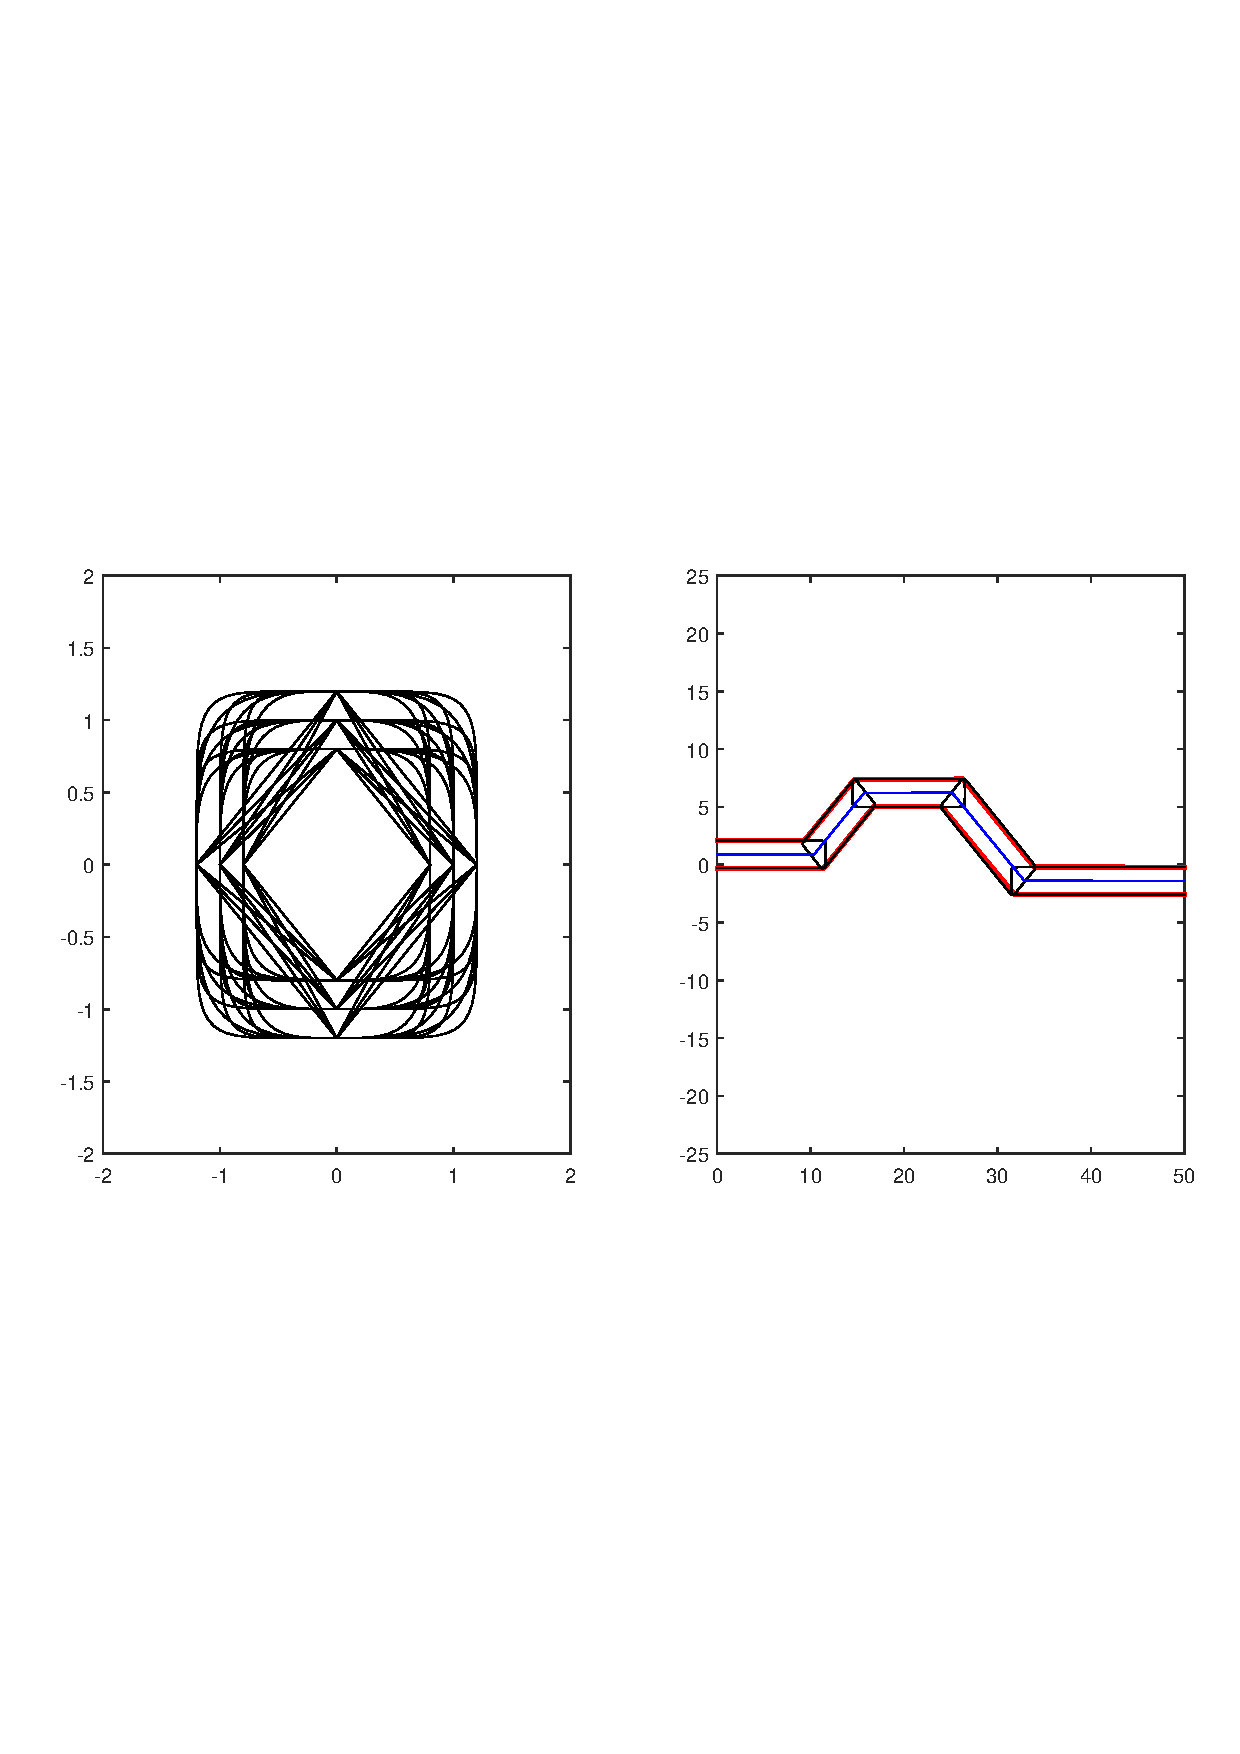
\includegraphics[scale=0.75]{figures/fig4.pdf}
\caption{ Super-ellipses and a duct modelled as combination of super-ellipses\label{fig:super-ellipses}}
\end{figure}

The condition $f(\textbf{x}_t)<0$ will ensure that the co-ordinates of the tail of the link $(x_t,y_t)$ always lie inside the bounding curve of a super-ellipse. However, in case of multiple equations (${f_i(x)},~ i=1,2,...,m$), only one of them will be satisfied for the point to be inside the duct. In practical implementation, we can say that this translates to saying that the least value amongst all the values of ${f_i(x)}$ should be less than zero. For the $i^\text{th}$ super-ellipse which is rotated by an angle $\phi_i$ about the $z-$ axis and whose center is translated to the co-ordinates $(x_i,y_i)$ so as to fit a portion of a duct, the co-ordinates of boundary should be multiplied with a transformation matrix
\begin{align}
T_i = \begin{bmatrix}
\cos \phi_i & -\sin\phi_i & 0 & x_i\\
\sin \phi_i & \cos\phi_i & 0 & y_i\\
0 & 0 & 1 &0\\
0 & 0 & 0 & 1
\end{bmatrix}
\end{align}
The constraint equation now becomes $g_i(\textbf{x}_t) : f_i(T_i^T\textbf{x}_t)< 0,~ i=1,2,...,m$. For practical implementation, we can write the inequality constraint as 
\begin{align}
\label{eq: min_and_mingx}
C_{\text{ineq}}:~~ \min\left(g_i(\textbf{x}_t)\right) < 0,~~ i=1,2,...,m 
\end{align}

An example of single link and multi-segmented chain passing through the duct is shown in [fig5]. Motion of a unit link with and without constraint is shown in [fig6]. The negative gradient (descend direction) of the inequality constraint function is also shown in the figure. The method shown here is quite fast and scalable as explained in section ??, while the majority of time taken for the scheme being in identifying the super-ellipsoids which fit the duct profile. For the example shown in this section, this identification is done by manually selecting clusters of points in the duct and fitting ellipses which will reduce the fitting error in a least squared sense.

%\begin{figure}[h]
%\centering
%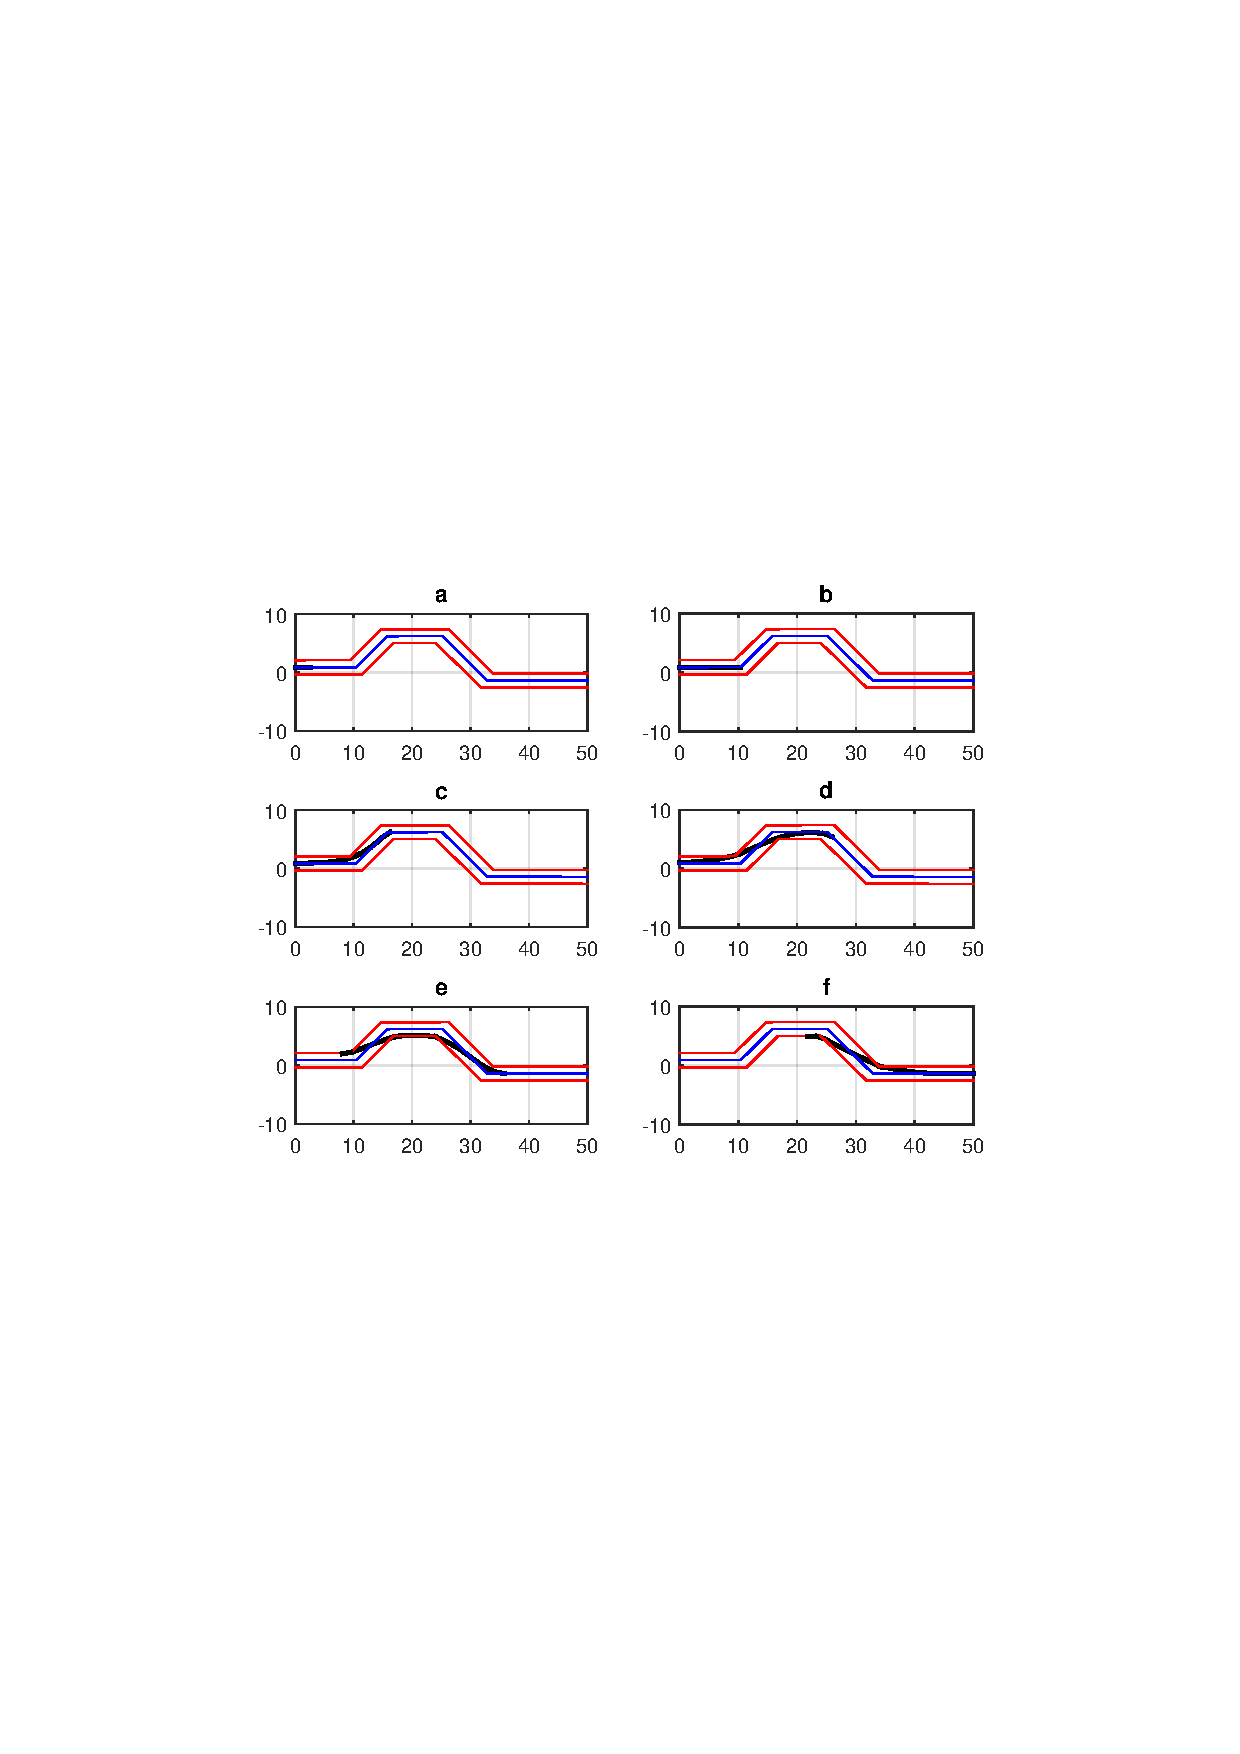
\includegraphics[scale=0.75]{figures/fig5.pdf}
%\caption{ Motion through duct modelled as combination of super-ellipses\label{fig:ductasSEs}}
%\end{figure}
%
%\begin{figure}[h]
%\centering
%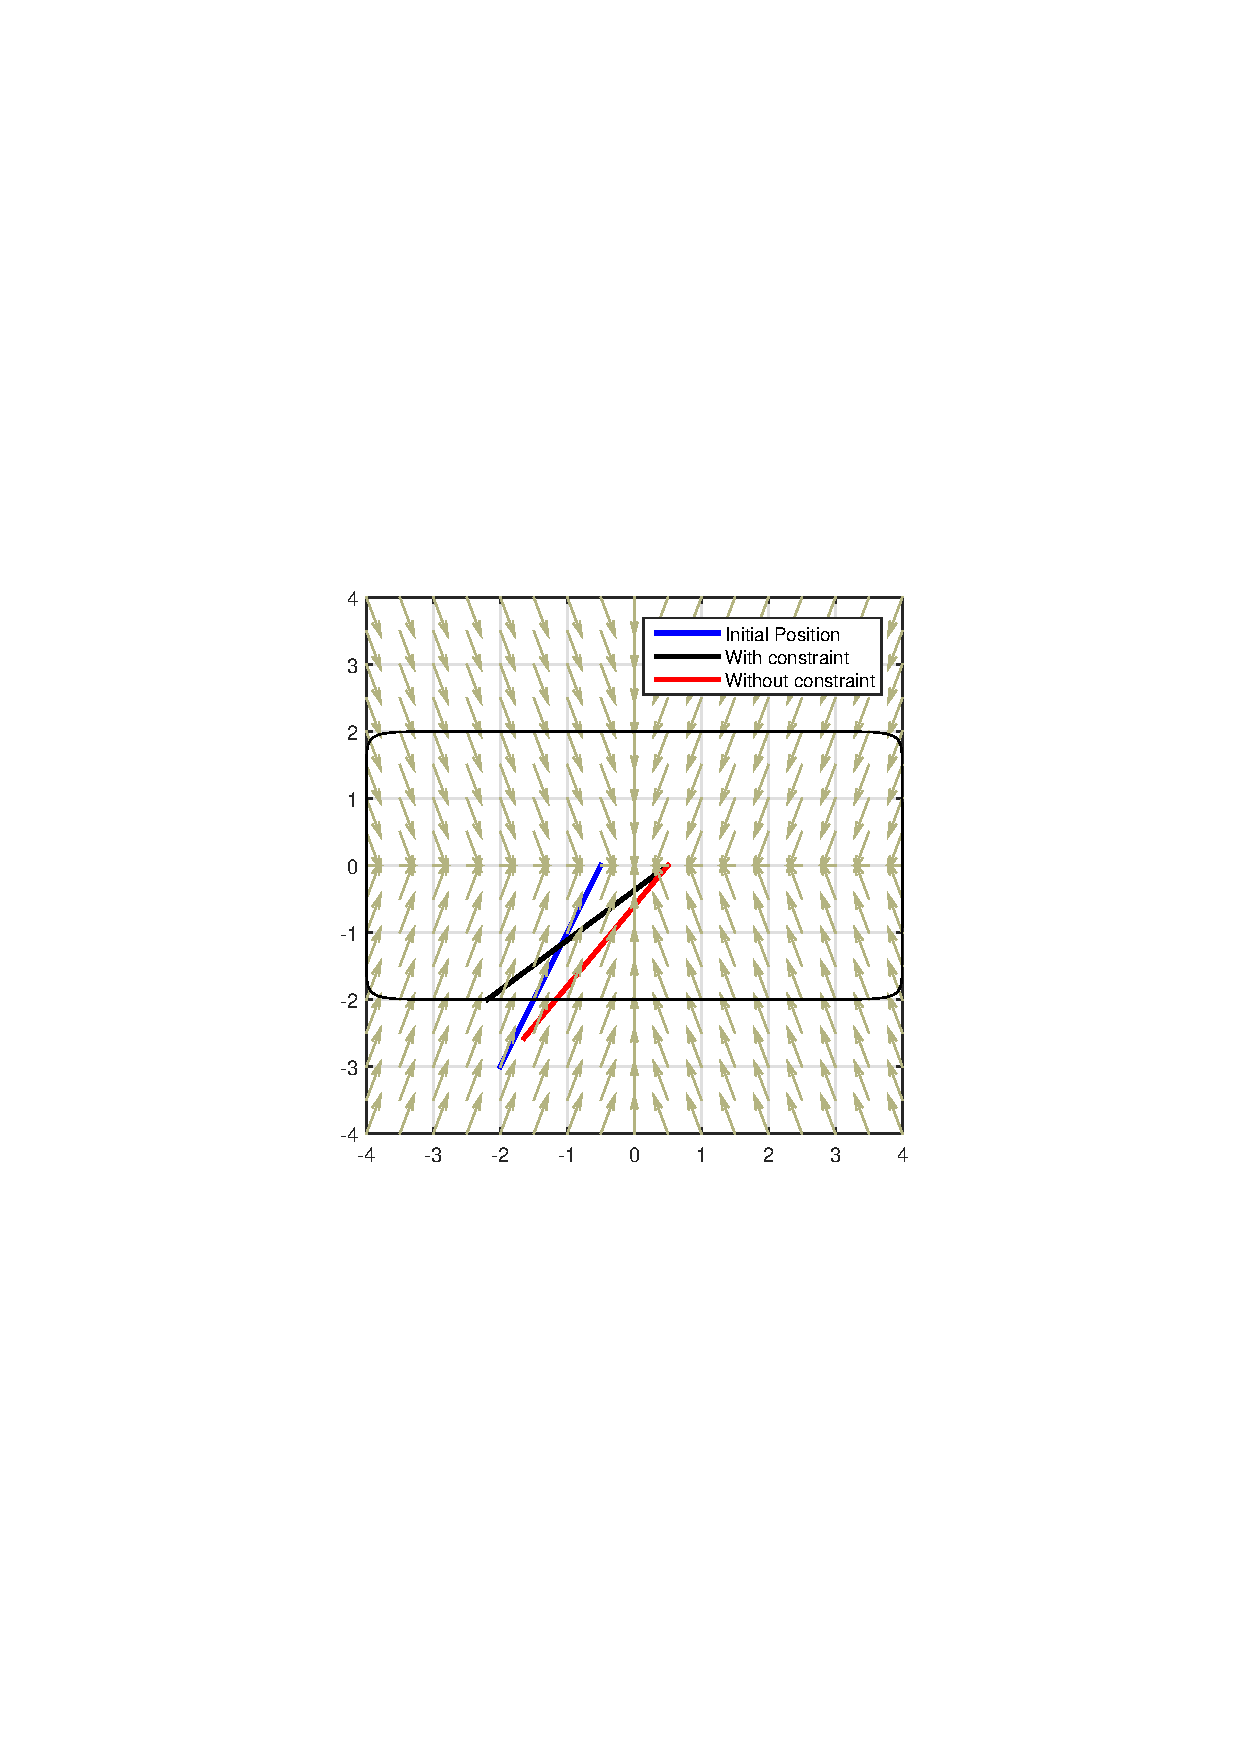
\includegraphics[scale=0.5]{figures/fig6.pdf}
%\caption{ Effect of gradient of inequality constraint in pulling the tail into the duct\label{fig:gradienteffectSE}}
%\end{figure}

\begin{figure}[ht!]
    \centering
    \begin{subfigure}{0.48\textwidth}
        \centering
        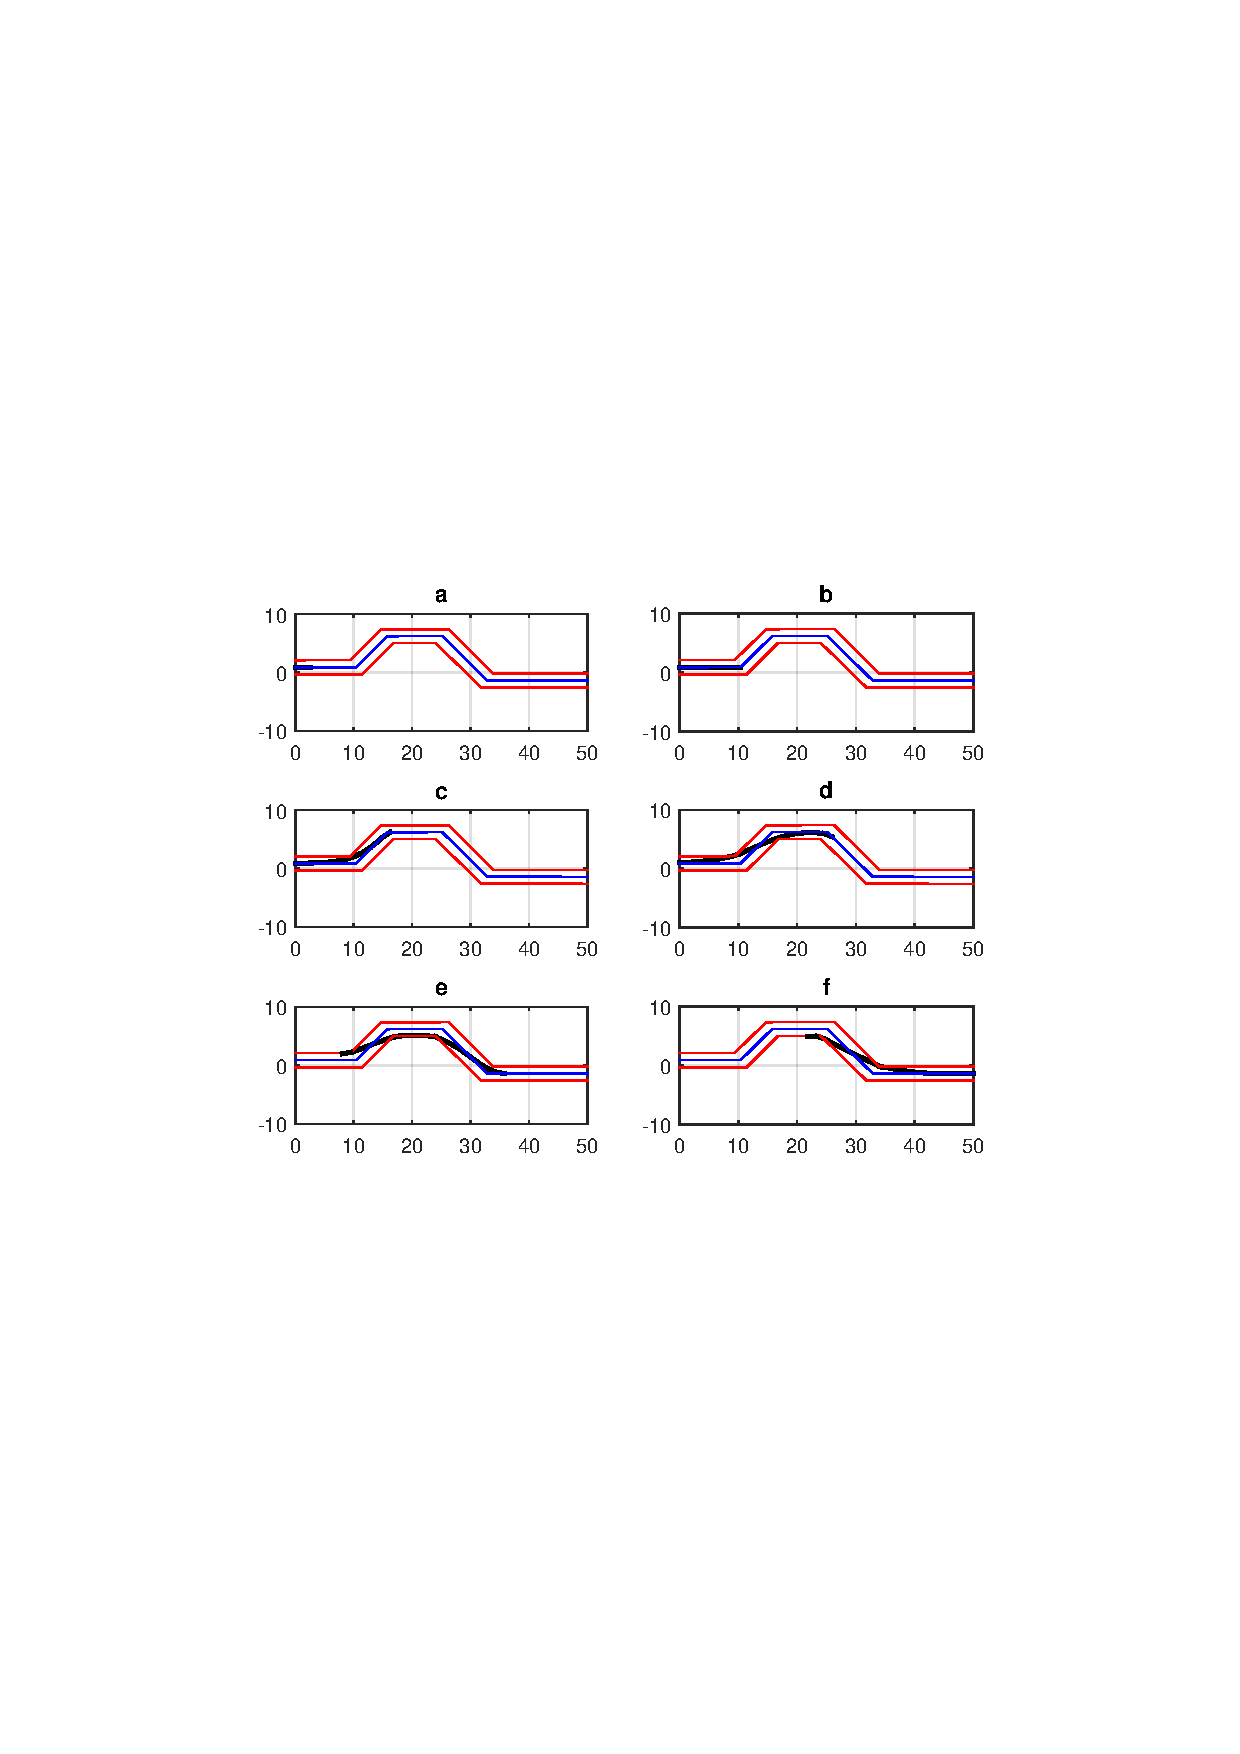
\includegraphics[width=0.95\linewidth]{figures/fig5.pdf}
        \caption{Motion through duct modelled as \\combination of super-ellipses \label{fig:ductasSEs}}
    \end{subfigure}%
    \begin{subfigure}{0.48\textwidth}
        \centering
        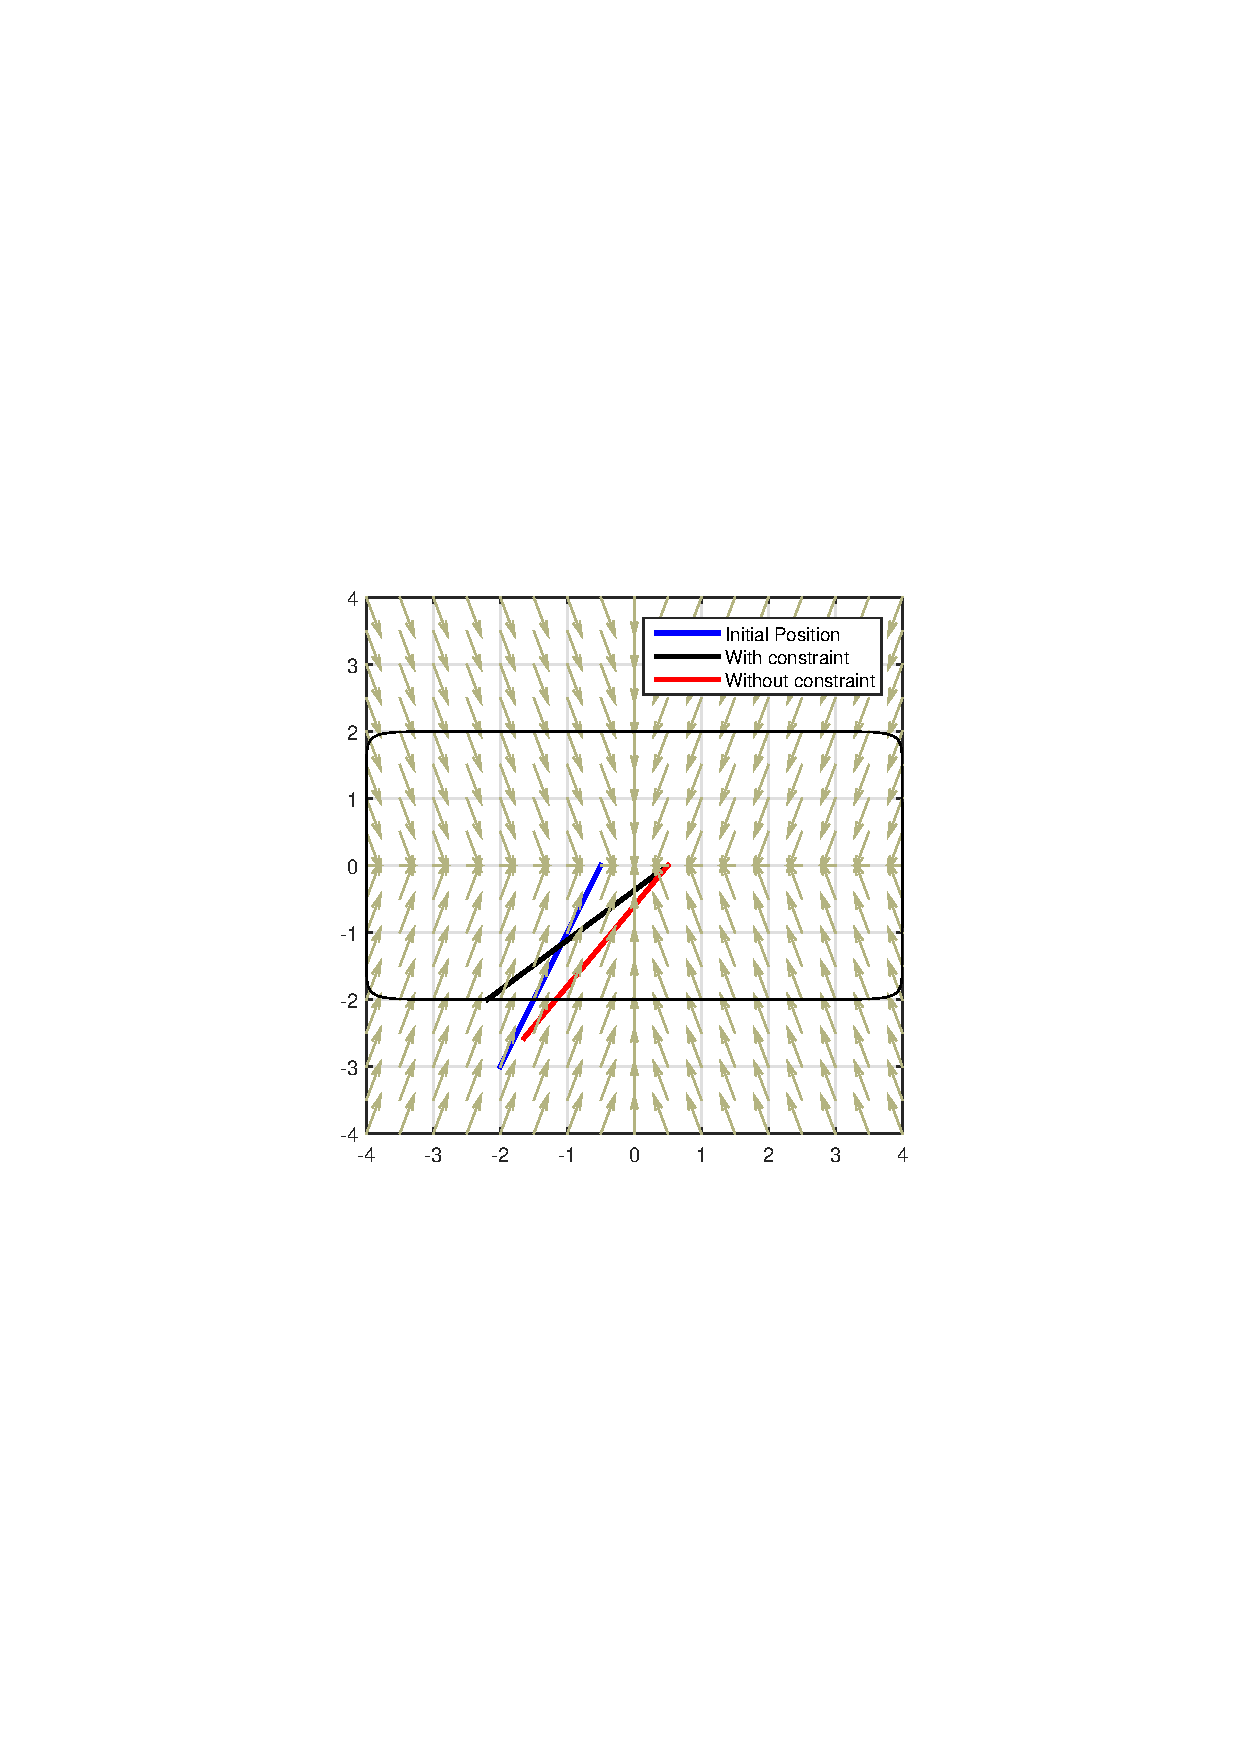
\includegraphics[width=0.75\linewidth]{figures/fig6.pdf}
        \caption{Effect of gradient of inequality constraint\\ in pulling the tail into the duct \label{fig:gradienteffectSE}}
    \end{subfigure}
    \caption{ Tractrix based algorithm on duct represented by ellipsoids}
\end{figure}


\subsection{Representation of duct as a set of connected quadrilaterals}

Since the profile of a super-ellipse is always symmetric, for complex and non-symmetric ducts, representation using the previous method might require a large number of shapes. For such cases, a complex duct shape can be represented as a closed shape obtained by stitching convex quadrilaterals as shown in \ref{fig:stitchequads}. The individual quadrilateral patches may be denoted as $A_1,A_2,...,A_n$, each bounded by the line segments defined by the points $\mathbf{(P_0,P_1),(P_1,P_2),...,(P_{n-1},P_n)}$ for the curve $\mathbf{\zeta_1}$ and $\mathbf{(Q_0,Q_1),(Q_1,Q_2),...,(Q_{n-1},Q_n)}$ for the curve $\mathbf{\zeta_2}$. Classification of a point $\mathbf{x}_t$ as inside or outside a quadrilateral represented by points, say, $\mathbf{P}_1,\mathbf{P}_2,\mathbf{Q}_2$ and $\mathbf{Q}_1,$ is essentially checking the placement of the point in the half spaces represented by the four lines spanned by the point set $\left(\mathbf{P}_1,\mathbf{P}_2\right)$, $\left(\mathbf{P}_2,\mathbf{Q}_2\right)$, $\left(\mathbf{Q}_2,\mathbf{Q}_1\right)$, and $\left(\mathbf{Q}_1,\mathbf{P}_1\right)$. This can be written as a set of four inequality constraints:
\begin{align}
A^1_i x_t+ A^2_i y_t +B_i <0 ~~ i=1,2,3,4\\
\end{align}
where $A_i^1 x+A_i^2y+B_i=0$ represents a line obtained from one pair of non-diagonal points in the quadrilateral. In matrix form, the inequality will look like:
\begin{align}
C_\text{ineq}:~~ \left[\mathbf{A} \right] \mathbf{x}_t +\mathbf{B} <0
\end{align}
where $\left[\mathbf{A} \right]$ is a $4\times 4$ matrix and $\mathbf{B}$ is a $4 \times 1$ vector.
But we propose a more convenient method for practical applications which is as follows:

The co-ordinates of a point inside the surface patch $A_i$ is given by the parametric expression
\begin{align}
\label{eq:xi(u,t)}
\mathbf{x}_i(u,v)= \left[ \mathbf{P}_{i-1}+\left(1-{u} \right)\mathbf{P}_i  \right]\left(1-{v}\right) +\left[\mathbf{ Q}_{i-1}+\left(1-{u} \right)\mathbf{Q}_i  \right]\left({v}\right)
\end{align}
in parameters $u$ and $v$. If the vertices of the quadrilateral are given by $\mathbf{P}_{i}=\left[ {}^xP_{i},{}^yP_{i}\right]^T $ and $\mathbf{Q}_{i}=\left[ {}^xQ_{i},{}^yQ_{i}\right]^T $, then the analytical expressions for the terms $u$ and ${v}$, given the value of $\mathbf{x}_i$, can be obtained by solving \ref{eq:xi(u,t)} (see Appendix). The values of $u,v$ can be used to classify the point with respect to the surface patch $A_i$\footnote{It may be noted that there will be two sets of solution and they are not always real and unique. For example, the point $\mathbf{P} =\left(10,-5 \right)$ when classified with respect to the area $A$ given by the points $\mathbf{P}_1 = \left(0,15 \right),\mathbf{P}_2 = \left(10,10 \right),\mathbf{Q}_1 = \left(0,0 \right)$ and $\mathbf{Q}_2 = \left(4,1 \right),$ returns the values $u=\left( 1.0 + 0.6~i,~1.0 - 0.6~i \right)$ and $v=\left(2.0 + 1.9~i,~2.0 - 1.9~i\right)$. However, it is easy to filter out the imaginary set of solutions, should the algorithm encounter the same.}.

\begin{figure}[h]
\centering
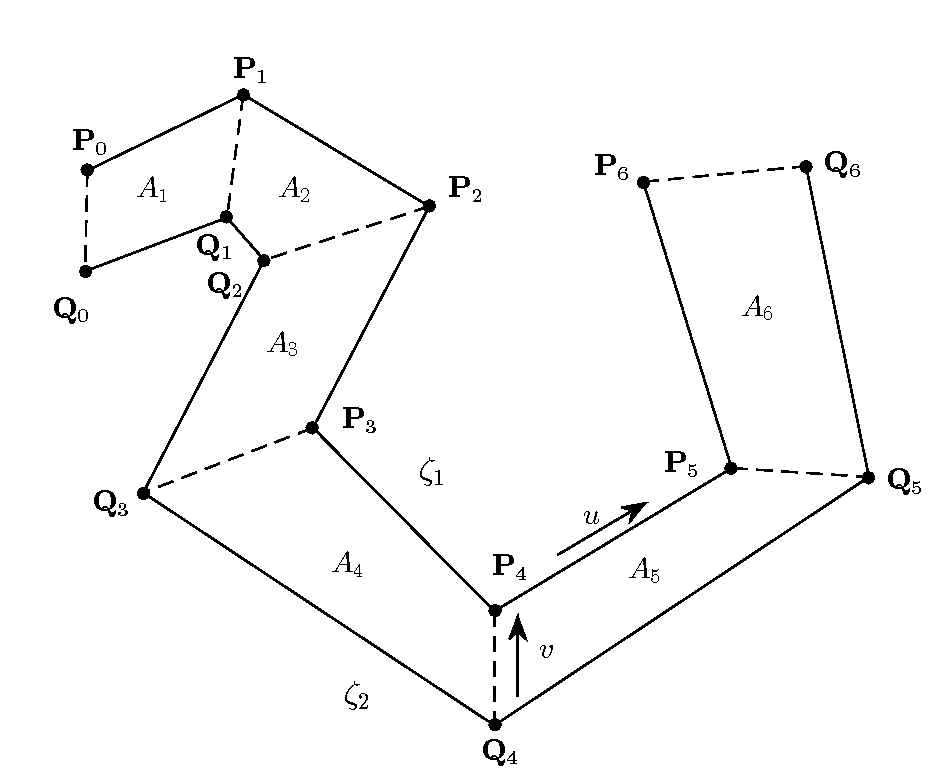
\includegraphics[scale=0.5]{figures/fig7.pdf}
\caption{Duct represented by stitched quadrilaterals\label{fig:stitchequads}}
\end{figure}

 In case of a single quadrilateral patch, the inequality constraints will be simply,
 \begin{align} \label{eq:minx,u,v}
C_\text{ineq}:~~& 0 \leq u \leq 1 ,~~  0 < v < 1 
\end{align}
for real values of ${u}$ and ${v}$. In case of multiple patches, classifying one point with respect to all the patches return the values $\left({u}_1,{v}_1 \right), \left({u}_2,{v}_2 \right),...,\left({u}_m,{v}_m \right)$ etc. for the $m$ number of patches $A_1, A_2,..., A_m$ and consequently, $m$ set of conditions. But out of the $m$ condition sets, only one set should be satisfied since the point will belong to only one patch at a given instance of motion through the duct. Including a switching  statement in the optimization code will be inefficient especially when the point to be classified is close to the common boundary between two patches. 

In order to provide a gradient to the constraint which will direct the point into the duct, an inequality constraint is to be included as in the case of super-ellipses described in the previous subsection. If $\hat{u}$ and $\hat{v}$ represent the parameters obtained for a point $\mathbf{x}_t$ classified with respect to the quadrilateral $A_i$, $x_{\zeta_1}(t) = \mathbf{P}_{i-1}+\left(1-{\hat{u}} \right)\mathbf{P}_i$ and $x_{\zeta_2}(t) = \mathbf{Q}_{i-1}+\left(1-{\hat{u}} \right)\mathbf{Q}_i$ will give the two points on the duct boundary curves corresponding to the parameter $\hat{u}$. Then we can see that the quantity
\begin{align}
\label{eq:ductgradientinquad}
h = \Vert \mathbf{x}_{\zeta_1}-\mathbf{x}_t\Vert^2+\Vert \mathbf{x}_{\zeta_2}-\mathbf{x}_t\Vert^2-\Vert \mathbf{x}_{\zeta_1}- \mathbf{x}_{\zeta_2}\Vert^2
\end{align}
will always assign a negative real value for $h$ when point is inside the duct and a positive real value when the point is outside the duct. The value will be zero only at the boundaries. Hence, for an array of quadrilaterals, it is only necessary that the minimum value of the vector $\mathbf{h} = [{h}_1, {h}_2,...,{h}_m]$ should be negative for classifying the point with respect to the duct, as in the case of previous section. But as we can see, the inequality only takes into account the parameter variation across the boundaries (along the parameter $v$) and not in the direction of $u$. To account for the same, we make use of the function $\chi$ which is necessarily a linear combination of two Heaviside step functions $H(0)-H(1)$, defined as:

\begin{align}
\label{eq:chifunction}
\chi(t) = \left\lbrace \begin{matrix}
0,&\quad t<0 \\
1,&\quad 0\leq t \leq 1\\
0, &\quad t >1
\end{matrix}\right.
\end{align}
The function $\chi$ applied on the quantity $\hat{u}_i$ (which is the value of parameter ${u}$ classified with respect to quadrilateral $A_i$), will return 0 only if the point satisfies the constraint $0\leq \hat{u}_i\leq 1$. Now, multiplying this quantity $\chi(\hat{u})$ with $h_i$ will return a non-zero negative value only if the point is inside the duct. Then the following inequality constraint:
\begin{align}
\label{eq:quadrils}
C_{\text{ineq}}:~~\left[\chi\left(\hat{\mathbf{u}}\right)\right]^T\mathbf{h}<0
\end{align}
where $\hat{\mathbf{u}}=\left[\hat{u}_1,\hat{u}_2,...,\hat{u}_m\right]^T$ becomes a more practical and convenient way to implement the inequality constraint in the optimization problem.

As an example, motion of a unit link passing through the duct is shown in [fig11] and the effect of the added inequality constraint~\ref{eq:quadrils} to pull the tail end of the link which is initially positioned outside the duct, is shown in [fig12]. Apart from being more flexible, another advantage of representing a 2D duct as a set of connected quadrilaterals in this parameteric form is that by setting the limits of the parameter $v$ to $0+\delta < v< 1-\delta,~~\delta<0.5$, it is easy to manually add a clearance from the walls of the duct without manipulating the duct itself. Also, it is easy to note that $\delta=0.5-\epsilon$ (where $\epsilon$ is a small number) would follow the backbone curve motion.

\begin{figure}[h]
\centering
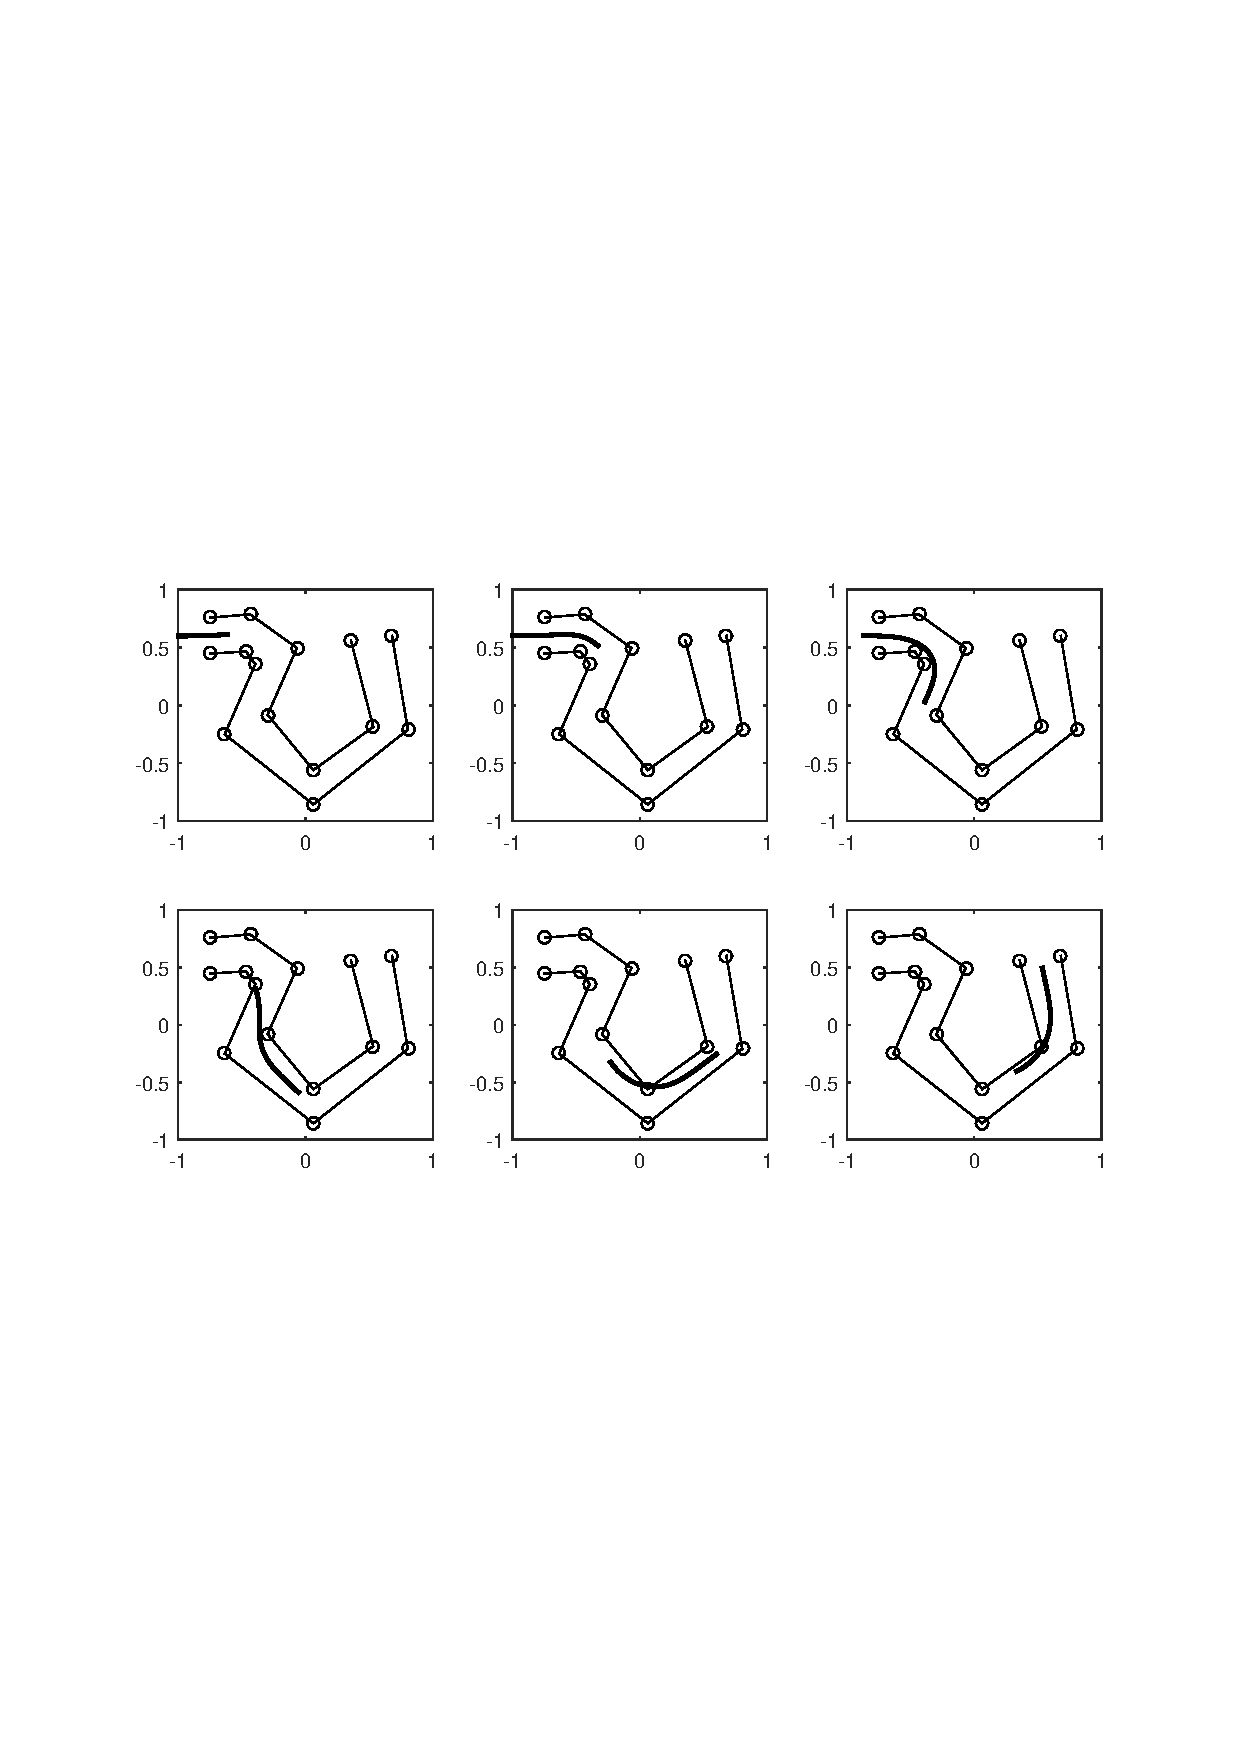
\includegraphics[scale=0.75]{figures/fig10.pdf}
\caption{ Example of constrained motion with stitched quadrilaterals \label{fig:motionquads}}
\end{figure}

\begin{figure}[h!]
\centering
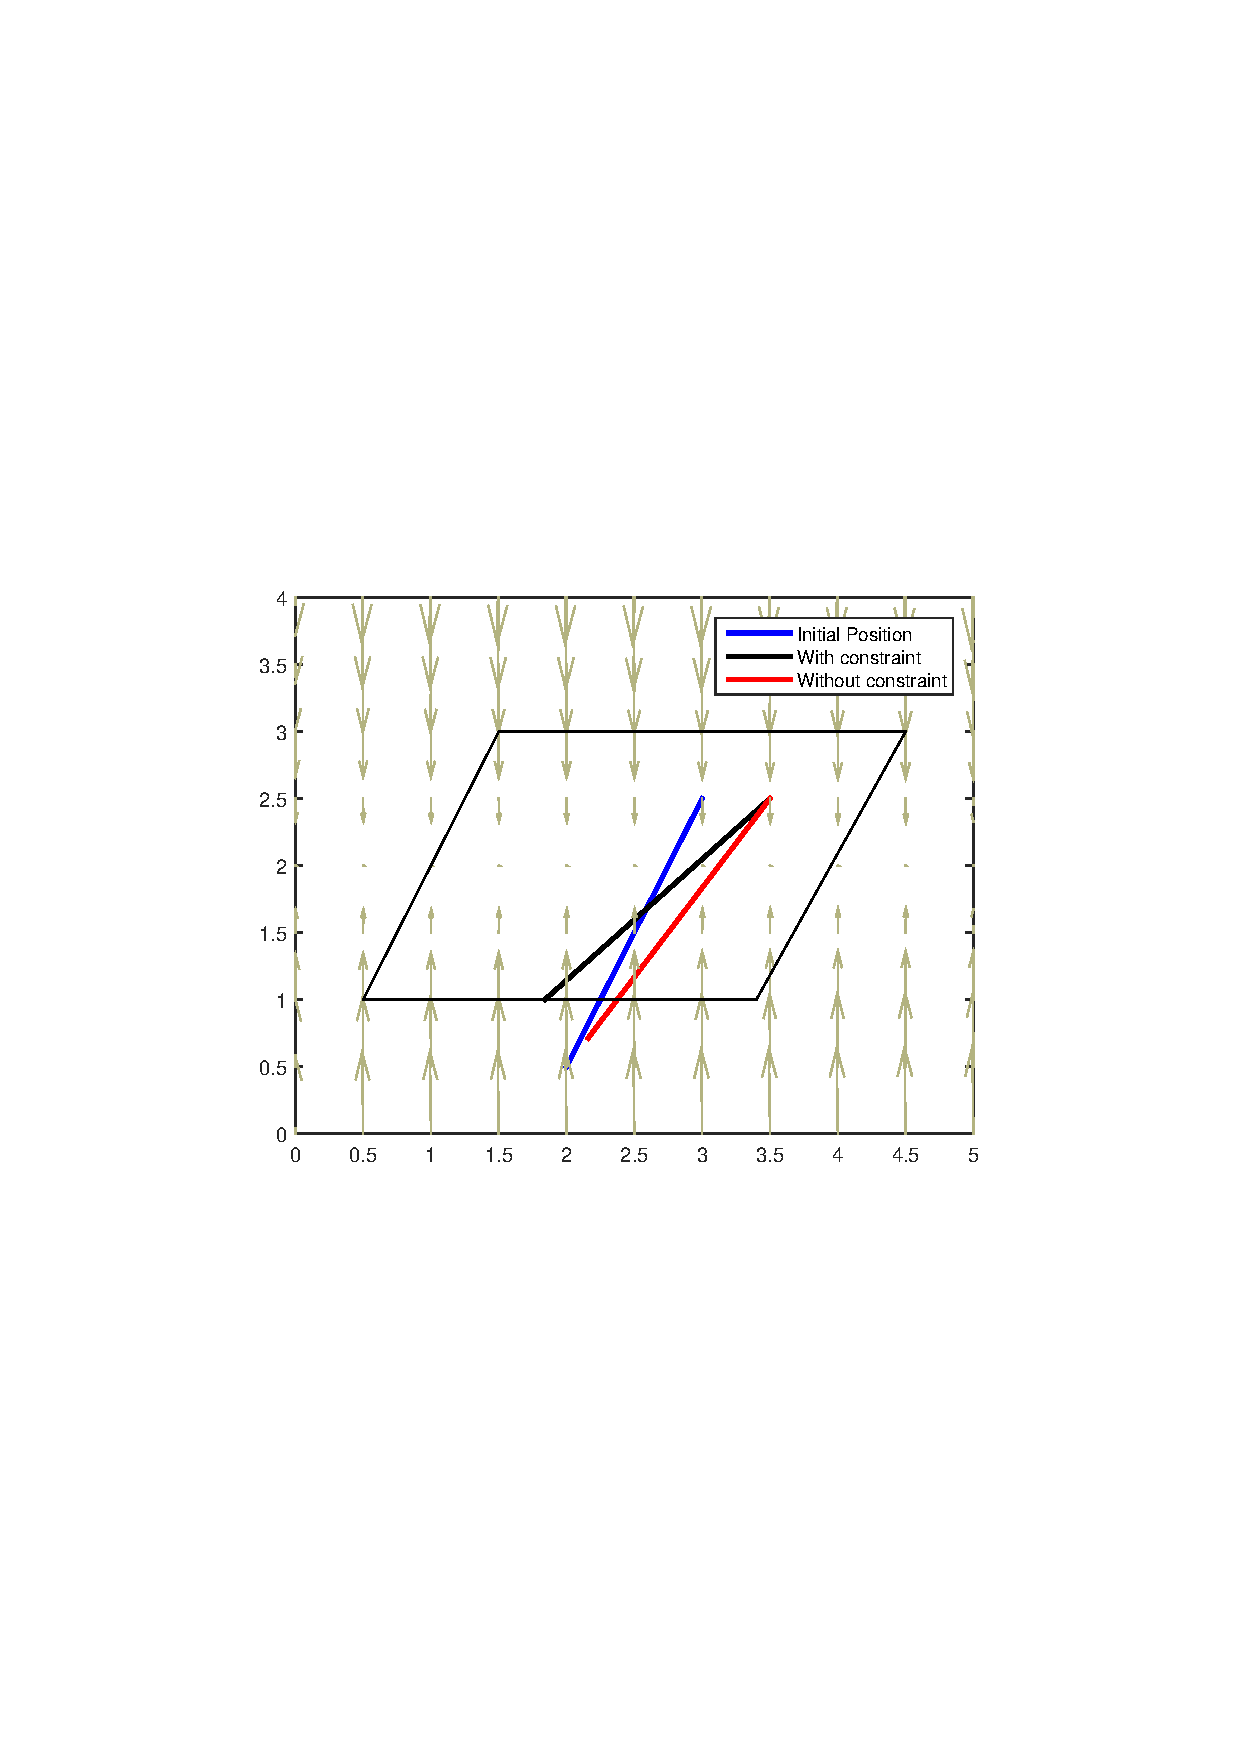
\includegraphics[scale=0.5]{figures/fig10b.pdf}
\caption{ Effect of gradient of inequality constraint in pulling the tail into the quadrilateral duct \label{fig:quadgradient}}
\end{figure}


\subsection{Representation of duct using two non-intersecting continuous curves}
If the non-intersecting border curves of the duct can be analytically expressed, then the equation of the surface patch will simply be,
\begin{align}
\mathbf{x}_i(u,v)= \zeta_1(u)\left(1-{v}\right) +\zeta_2(u)\left({v}\right)
\end{align}
For example, [fig11] shows a 2D duct defined by two curves $\zeta_1(u) = \left[u,~\sin\left(u \right)\right]^T$ and $\zeta_2(u) = \left[u,~\sin\left(u +\frac{\pi}{8}\right)+1\right]^T$ and a path chosen midway between the two curves. The equation of the surface generated by this curves will be

\begin{figure}[ht!]
    \centering
    \begin{subfigure}{0.48\textwidth}
        \centering
        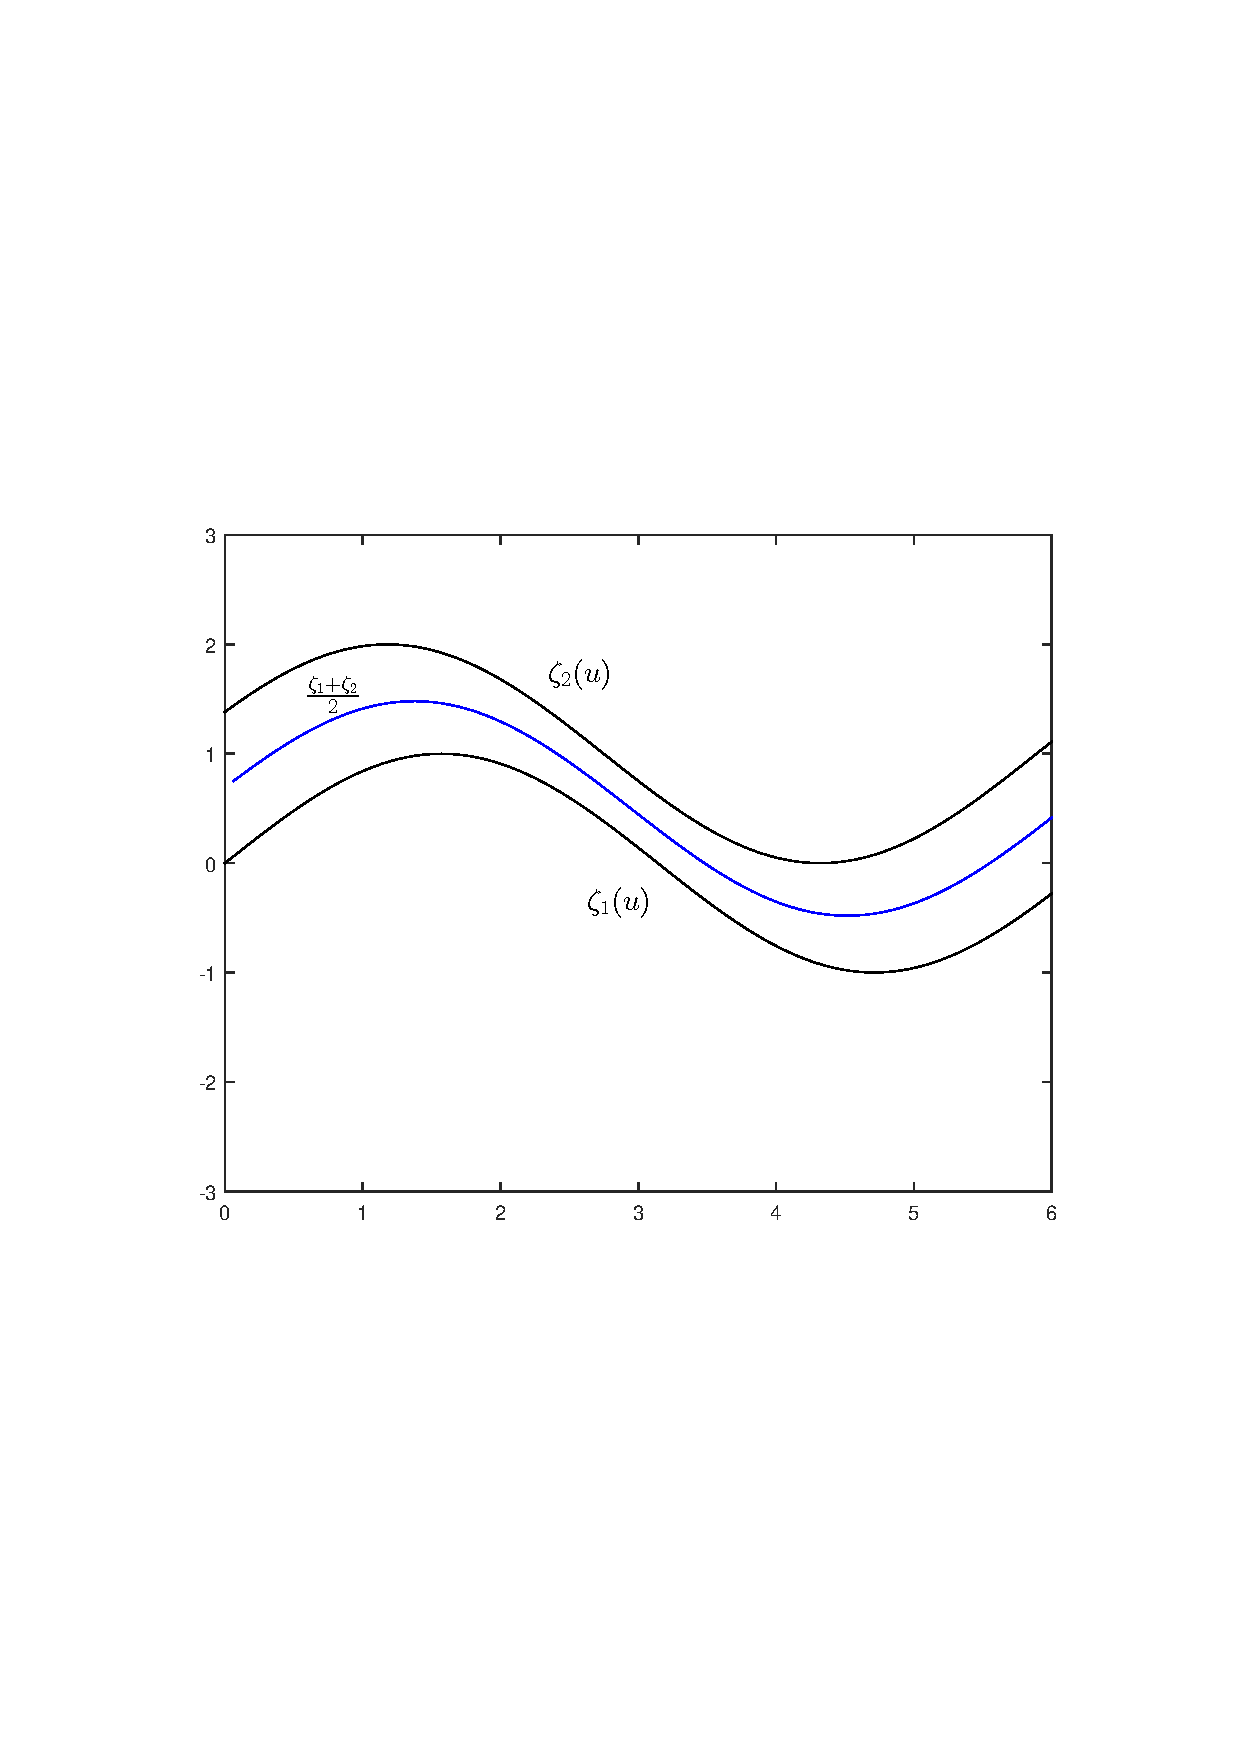
\includegraphics[width=0.75\linewidth]{figures/fig11.pdf}
        \caption{Example of analytical duct \label{fig:analyticduct}}
    \end{subfigure}%
    \begin{subfigure}{0.48\textwidth}
        \centering
        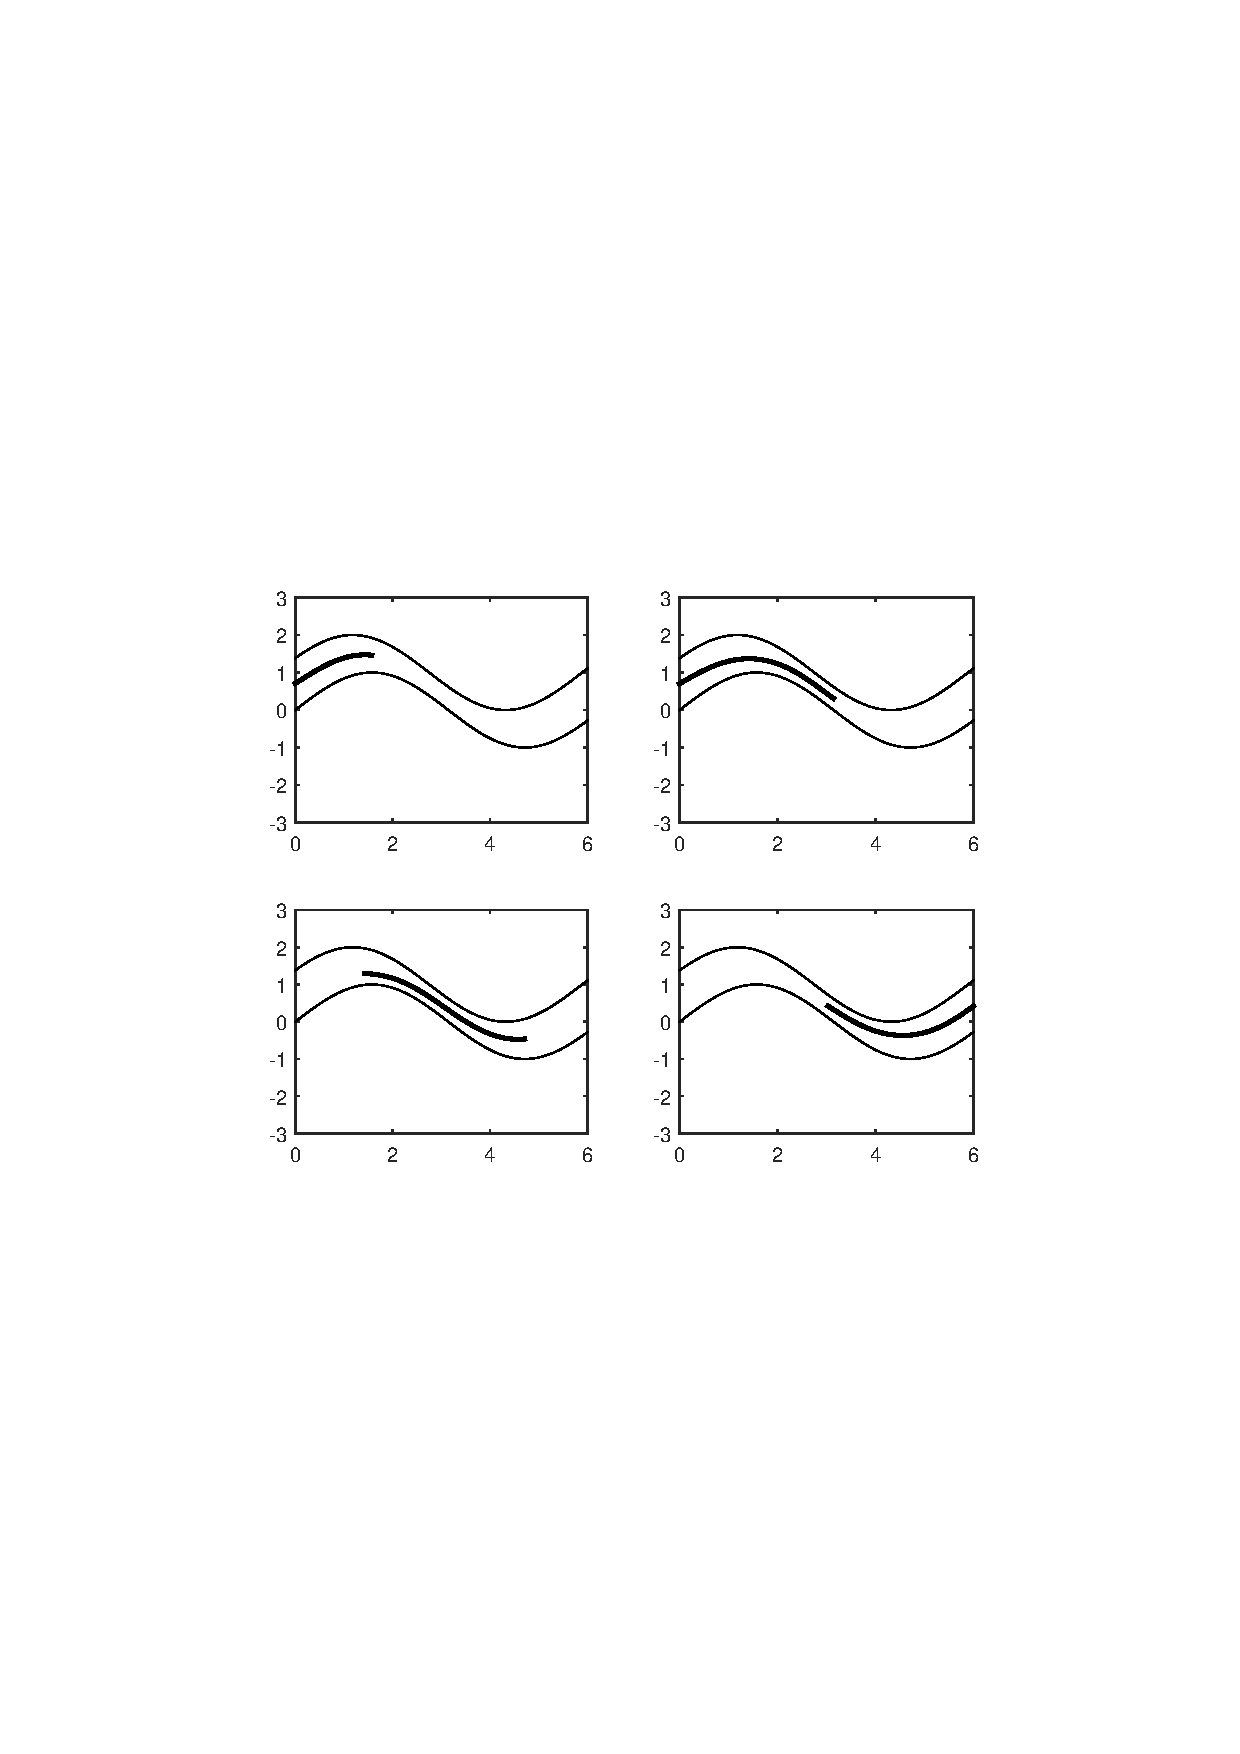
\includegraphics[width=0.75\linewidth]{figures/fig12.pdf}
        \caption{Motion through analytical duct \label{fig:analyticductmotion}}
    \end{subfigure}
    \caption{ Tractrix based algorithm on analytical duct}
\end{figure}


\begin{align}
\begin{bmatrix}
x(u,v)\\y(u,v)
\end{bmatrix} = 
\begin{bmatrix}
u\\\sin\left(u\right)+\left[\sin\left(u+\frac{\pi}{8}\right)-\sin\left(u\right)+1 \right]v
\end{bmatrix}
\end{align}
which has the analytical solution for $u$ and $v$:
\begin{align*}
u &= x\\
v &= \frac{y-\sin\left(x\right)}{\sin\left(x+\frac{\pi}{8}\right)-\sin\left(x\right)+1}
\end{align*}
In this case, we will solve the equations:
\begin{align}
\label{eq:analy2D}
\min_{\textbf{x}_t} &\Vert \textbf{x}_t-\textbf{X}_t \Vert\\
\nonumber \text{sub:~~~} &\Vert \textbf{x}_h - \textbf{x}_t \Vert -L_0 = 0\\
&0< v\vert_{\mathbf{x}_t}< 1
\end{align} 
 An example movement of hyper-redundant manipulator through the duct is shown in [fig12]. However, analytical solution is not always viable for complex equations and numerical procedure must be employed to find the values of $u$ and $v$ corresponding to the given tail point to be classified. Also, since multiple solutions may be possible for such cases, the correctness of the solution would heavily depend on the choice of initial guess provided\footnote{The same argument will also hold for analytical surfaces spanned in 3D and hence is not studied further.}. The equation to be used is \ref{eq:minx,u,v}.

%----------------------------------------------------------------------------------------------------
\section{Motion planning through 3D ducts}
\label{sec:3Dmotionplanning}
In this section, we will explain a few methods to represent ducts in 3D and how motion planning is achieved in the same.
\subsection{Representation of duct using combination of super-ellipsoids}
In Cartesian co-ordinate system in $R^3$, the surface of a super-ellipsoid follows the equation:
\begin{equation}
f(x,y,z) : \left[ \left\lbrace \left(\frac{x}{a} \right)^{\frac 2e} +\left(\frac{y}{b} \right)^{\frac 2e} \right\rbrace^{\frac{e}{n}} +\left(\frac{z}{c} \right)^{\frac 2n}  \right]^\frac n2-1 =0
\end{equation}


By changing the parameters $a,b,c$ and $n$, we get different closed surfaces as shown in [fig13]. By combining different super-ellipse shapes, we can generate a 3D duct as shown in [fig14]

\begin{figure}[h!]
\centering
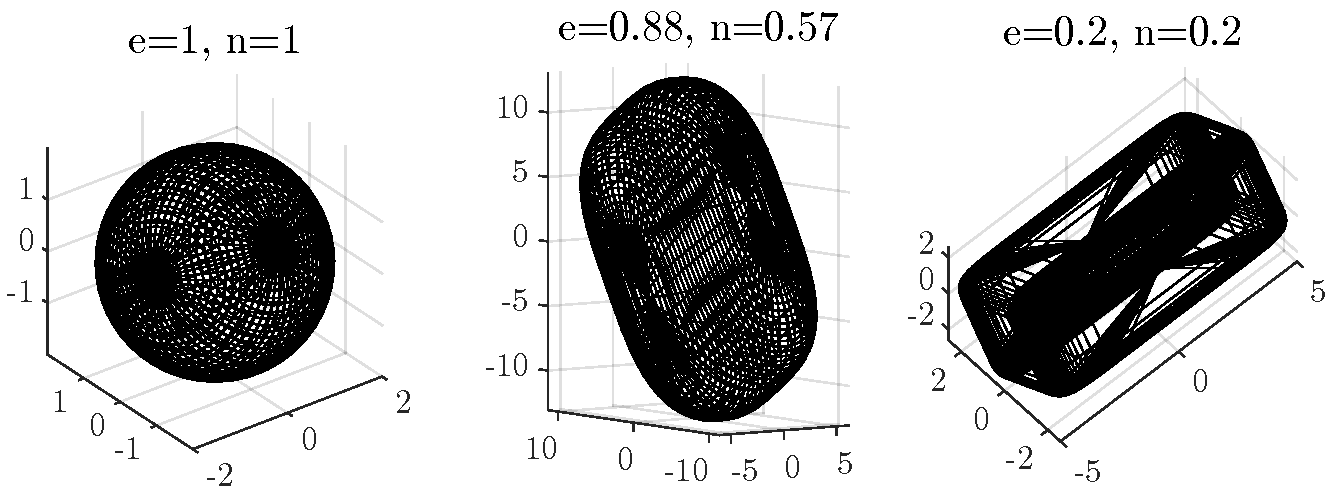
\includegraphics[scale=0.5]{figures/fig13.pdf}
\caption{ Super-ellipsoids \label{fig:SEs}}
\end{figure}

The procedure to calculate the inside-outside condition is same as that of the method described in section [ref sec]. The inequality condition will be [\ref{eq: min_and_mingx}]. An example problem with duct approximated using super-ellipsoids is shown in [fig15]. As mentioned in the case for super-ellipses, solution to the motion planning problem with ducts represented by super-ellipsoids is fast (also explained in section ??). Identifying the shapes which fit the duct, is also same as the method mentioned in section ??. 

\subsection{Representation of duct as a set of connected cylinders}
Similar to the set of connected quadrilaterals in 2D, a duct in 3D can be represented by series of connected cylinders. By linearly interpolating two circles in space, we get the parametric equation of the cylinder as (refer Appendix for the detailed expressions):
\begin{align}
\label{eq:cylinder}
x = C_1(u,t,\theta),~~y = C_2(u,t,\theta),~~z = C_3(u,t,\theta)
\end{align}
where the parameters $u,t$ and $\theta$ varies along the radial, axial and circumferential direction of the cylinder respectively (refer [fig ??]). Similar to the representation in [sec], $0\leq u< 1$ and $0<t<1$ classifies the point as inside the cylinder. The constrained inequality \ref{eq:quadrils} generated will also be valid for cylinders. The quantity $h_i$ will simply be $h = \hat{u}_i-1$, which will show the same characteristics as defined by the value of $h_i$ in equation \ref{eq:ductgradientinquad}. The constraint inequality, hence takes the form:
\begin{align}
\label{eq:const_cyl}
C_\text{ineq}:~~\left[\chi\left(\hat{\mathbf{t}}\right)\right]^T\mathbf{h}<0
\end{align}
As is the case of quadrilaterals,it is possible to add a clearance from the walls by changing the radius of cylinder from $r$ to $r-\delta$, which is a very desirable characteristic for robots used in medical applications. 





\subsection{Representation of duct as point clouds}\label{sc:duct_as_STL}

The most direct way of representing the duct, in a practical sense, would be as a point cloud  ($\mathbf{R}_i,i=1,2,...,N$ where $N$ is the number of points in the cloud) such as obtained from a LiDAR system or a depth map. Subsequently, it would be possible to process the raw data to obtain the geometric representation of the point of cloud as a Stereolithographic formatted file (STL) or the like. Using the current framework, it is possible to pose the motion planning problem in the following form:
\begin{align}
\label{eq:STLeqs}
\min_{\textbf{x}_t} &\Vert \textbf{x}_t-\textbf{X}_t \Vert\\
\nonumber \text{sub:~~~} &\Vert \textbf{x}_h - \textbf{x}_t \Vert -L_0 = 0\\
&[\mathbf{A}]\mathbf{x}_t+\mathbf{B}\leq 0 \nonumber
\end{align}
where $\mathbf{A}$ is a $m\times 3$ matrix and $\mathbf{B}$ is a $m\times 1$ vector. The left hand side of $m$ inequalities represent the equations of $m$ number of planes spanned by three adjacent points in the cloud. The $i^\text{th}$ equation, $A_{i}^1x_t+A_{i}^2y_t+A_{i}^3z_t+B_i$ takes a value less than zero when the point $\mathbf{x}_t$ is in the half space which contains the origin and is greater than zero otherwise. The value also provides the attractive gradient which will ensure that the point stays inside the duct. However, in actual implementation, this procedure will be tedious and for practical convenience, it is possible to classify the point $\mathbf{x}_t$ as inside or outside the hull using the \cref{alg:in_hull} described in \cref{app:polyhedron_point}. The attracting gradient which ensures the point to be inside the duct--as the case with the previous methods-- can be provided using the artificial potential field generated from the centroid of the point cloud in conjunction with the output of the in-out function. The inequality constraint then becomes
\begin{align}
\label{eq:STLineq}
w(\mathbf{R})\frac{1}{\Vert(\overline{\mathbf{R}})-\mathbf{x}_t\Vert}\leq 0
\end{align}
where $w(\overline{\mathbf{R}})$ represents the output from in-out function which is either 1 for the point being outside and 0 for the point being inside the cloud or on the bounding surface\footnote{Unlike the previous classification problems, the bounding surface will also be considered as inside the surface in this case.}. 

Another interesting prospect of this method is its application in obstacle avoidance where the left hand side of the equation \Cref{eq:STLineq} will be greater than zero. The obstacle avoidance methods which follow the equation given by \Cref{eq:obstacle_avoidance_opt} is often limited to shapes which can be modelled analytically. Though the algorithm shown here is limited to convex shapes, they can be applied to more complex and non-symmetric shapes. Representation of pipe using ellipsoids, analytical cylinders and as convex point clouds is shown in \ref{fig:pipefitECS}.


\begin{figure}[ht!]
    \centering
    \begin{subfigure}{0.325\textwidth}
        \centering
        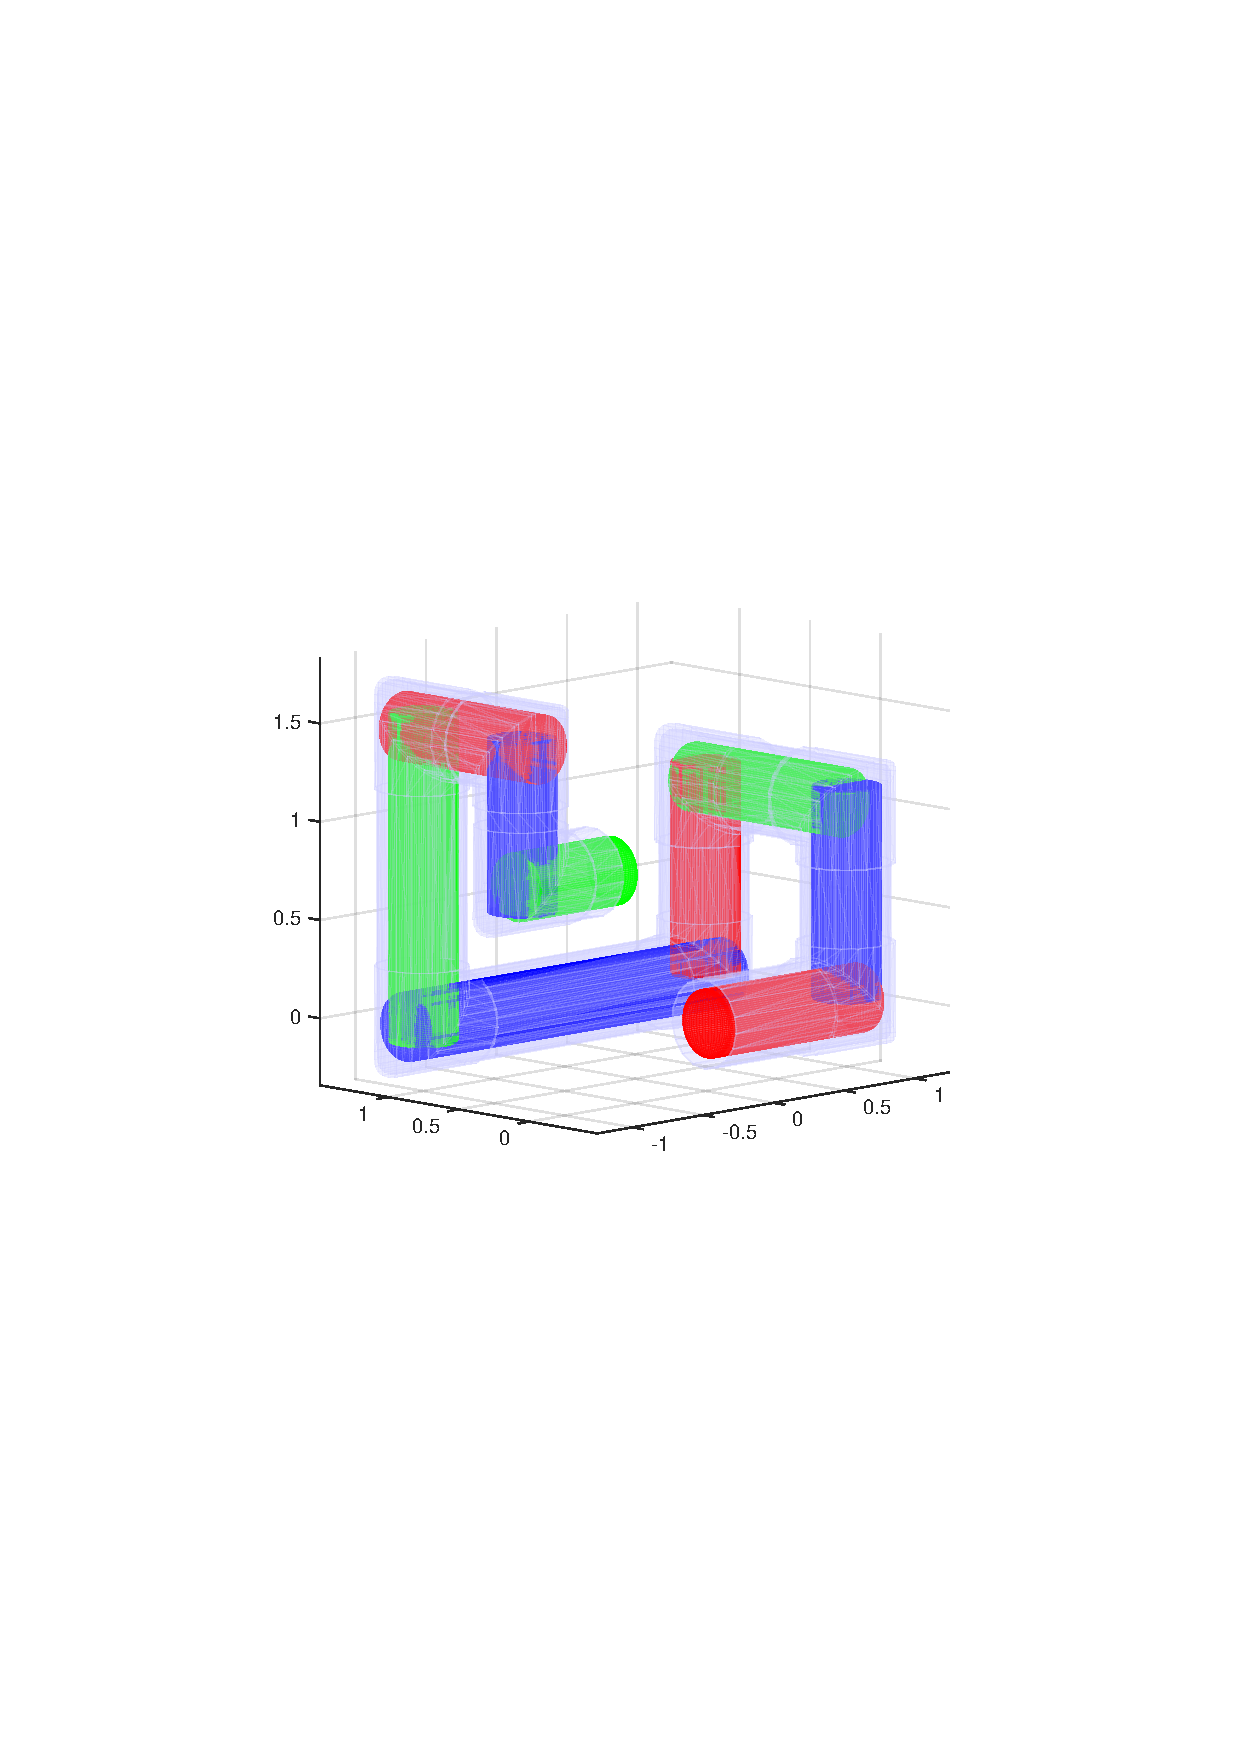
\includegraphics[width=0.75\linewidth]{figures/pipefitell.pdf}
        \caption{Ellipsoid fit \label{fig:pipefitell}}
    \end{subfigure}%
    \begin{subfigure}{0.325\textwidth}
        \centering
        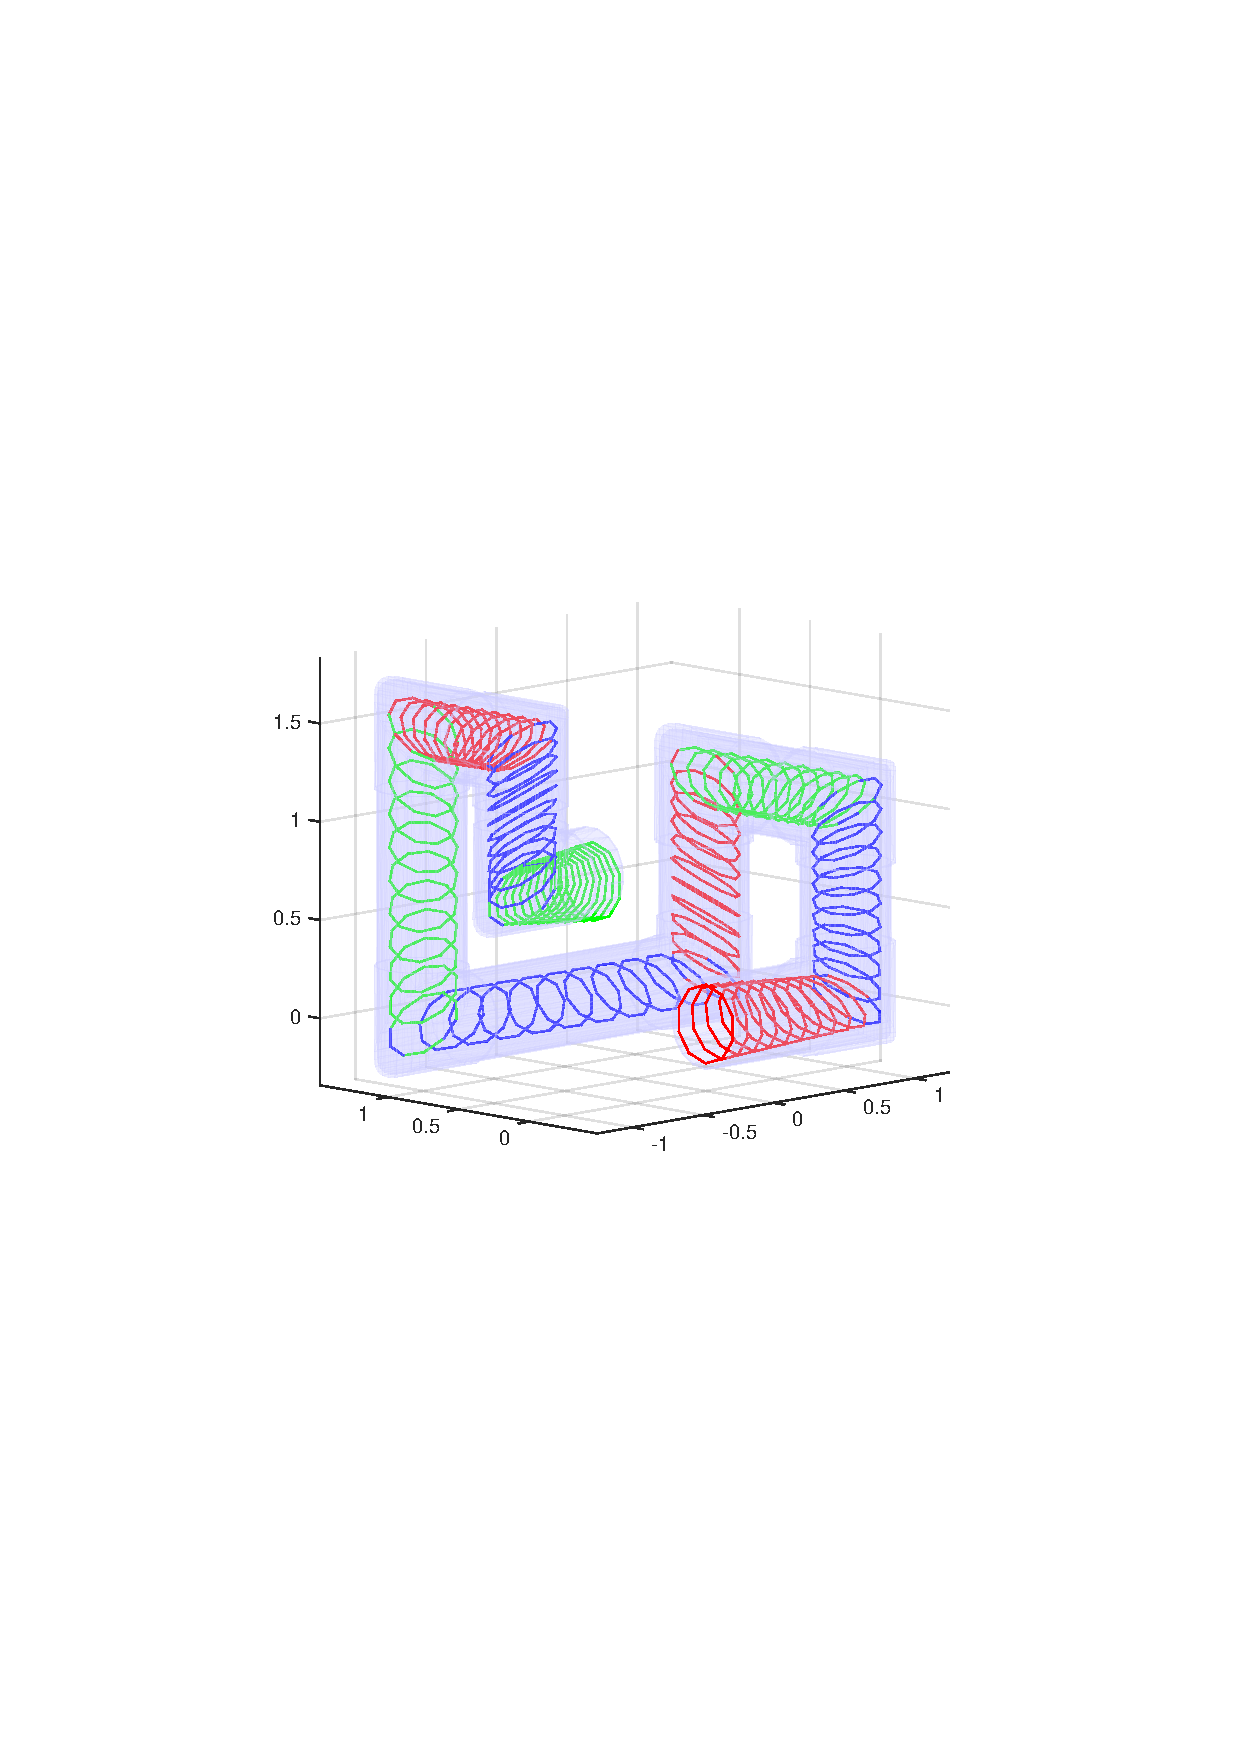
\includegraphics[width=0.75\linewidth]{figures/pipefitcyl.pdf}
        \caption{Cylinders fit \label{fig:pipefitcyl}}
    \end{subfigure}
        \begin{subfigure}{0.325\textwidth}
        \centering
        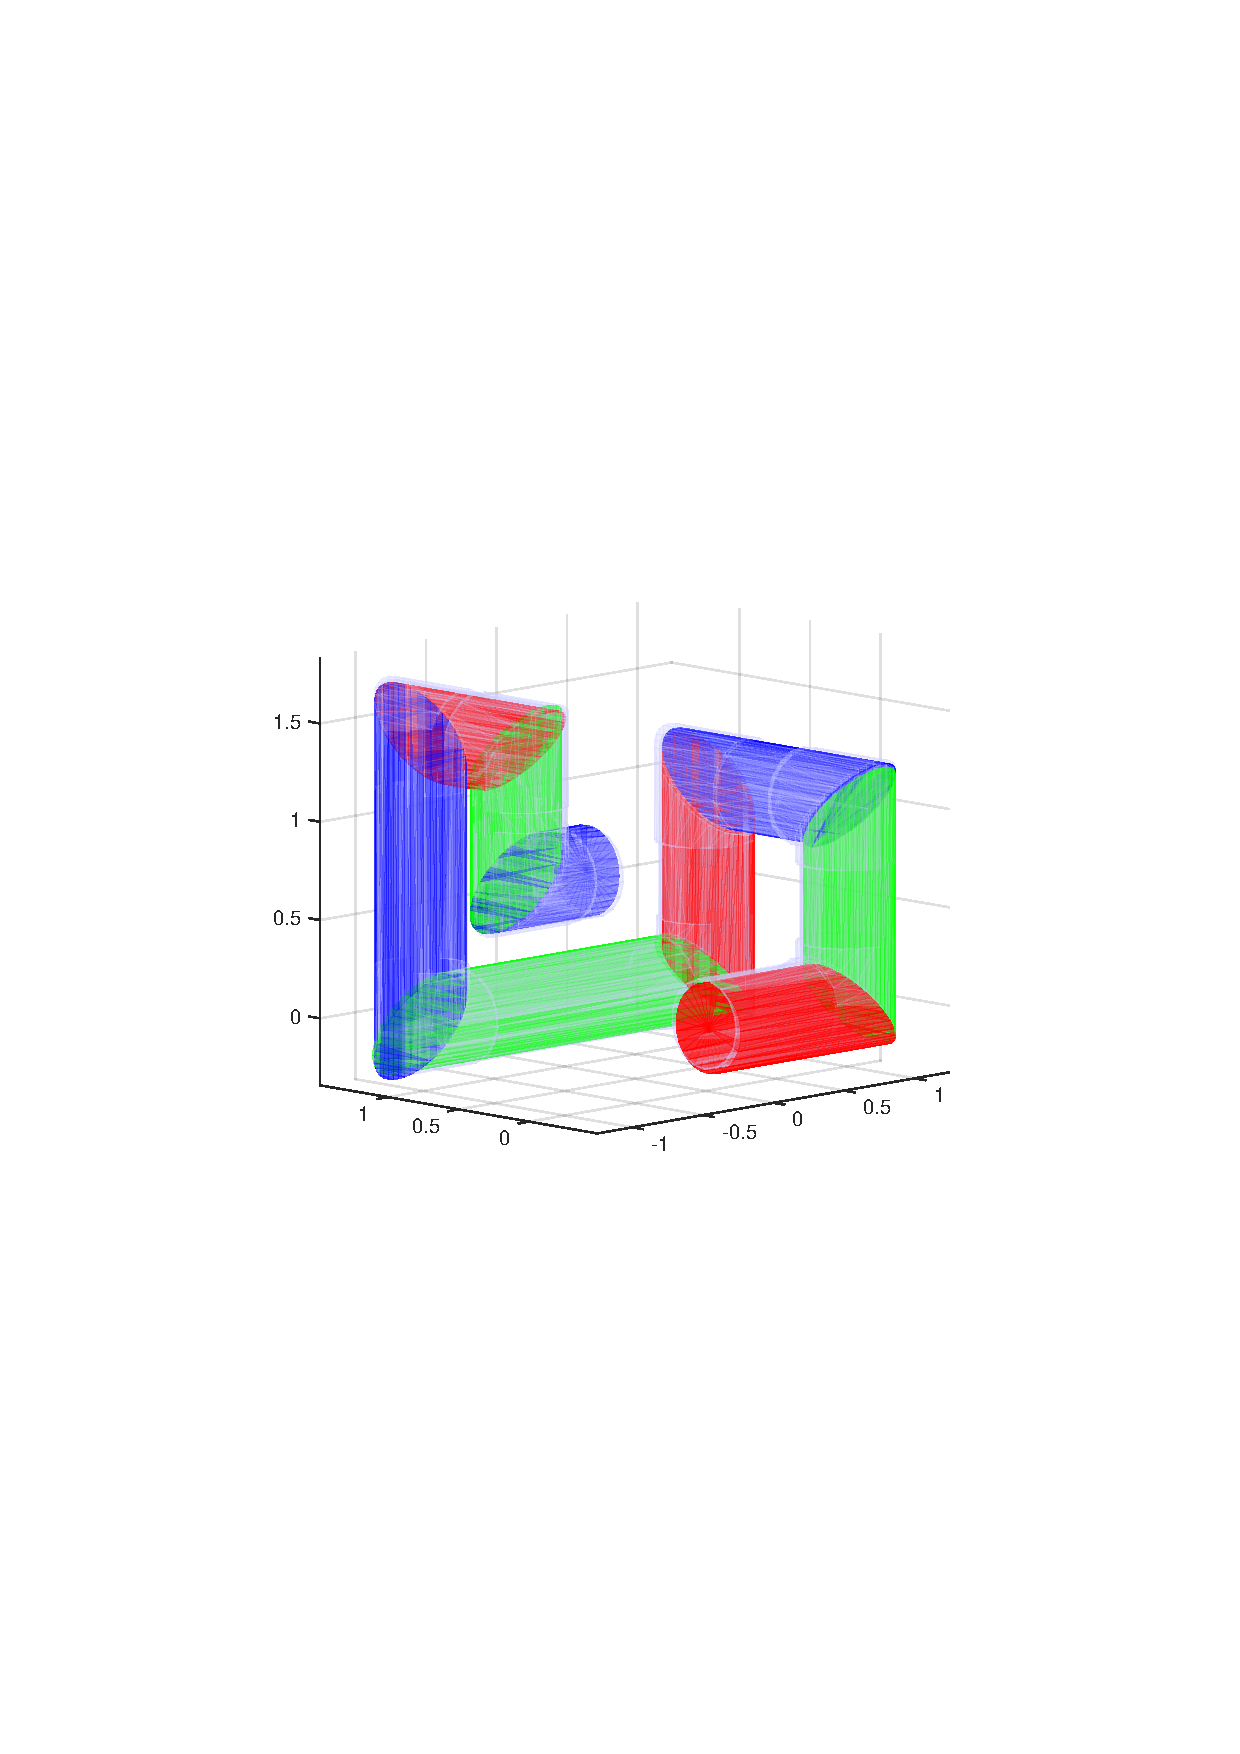
\includegraphics[width=0.75\linewidth]{figures/pipefitstl.pdf}
        \caption{Point clouds fit\label{fig:pipefitstl}}
    \end{subfigure}
    \caption{ Representation of duct using ellipsoids, cylinders and point clouds\label{fig:pipefitECS}}
\end{figure}

%\subsection{Analytical ducts}
%As mentioned in the section??, it is possible to express a few class of ducts using closed form expressions. For example, the helical duct shown in [fig ??] can be expressed using the equations
%\begin{align}
%\begin{bmatrix}
%x(u,\theta,\phi)\\y(u,\theta,\phi)\\z(u,\theta,\phi)
%\end{bmatrix} = 
%\begin{bmatrix}
%\left(R+ru\cos\theta \right)\cos\phi\\
%\left(R+ru\cos\theta \right)\sin\phi\\
%\left(R+r\sin\theta \right)+H\phi
%\end{bmatrix}
%\end{align}
%
%where $R,r,H$ are the radius of the helix, half the thickness of duct and the height of the helix respectively. The solution method involves solving the equation:
%\begin{align}
%\label{eq:analy3D}
%\min_{\textbf{x}_t} &\Vert \textbf{x}_t-\textbf{X}_t \Vert\\
%\nonumber \text{sub:~~~} &\Vert \textbf{x}_h - \textbf{x}_t \Vert -L_0 = 0\\
%&0\leq u < 1
%\end{align} 
%There exists multiple solutions to this equation and one has to conditionally check the validity of the solution while implementation. The motion of hyper-redundant robot through a helical duct is shown in fig??.

%
%\begin{figure}[h!]
%\centering
%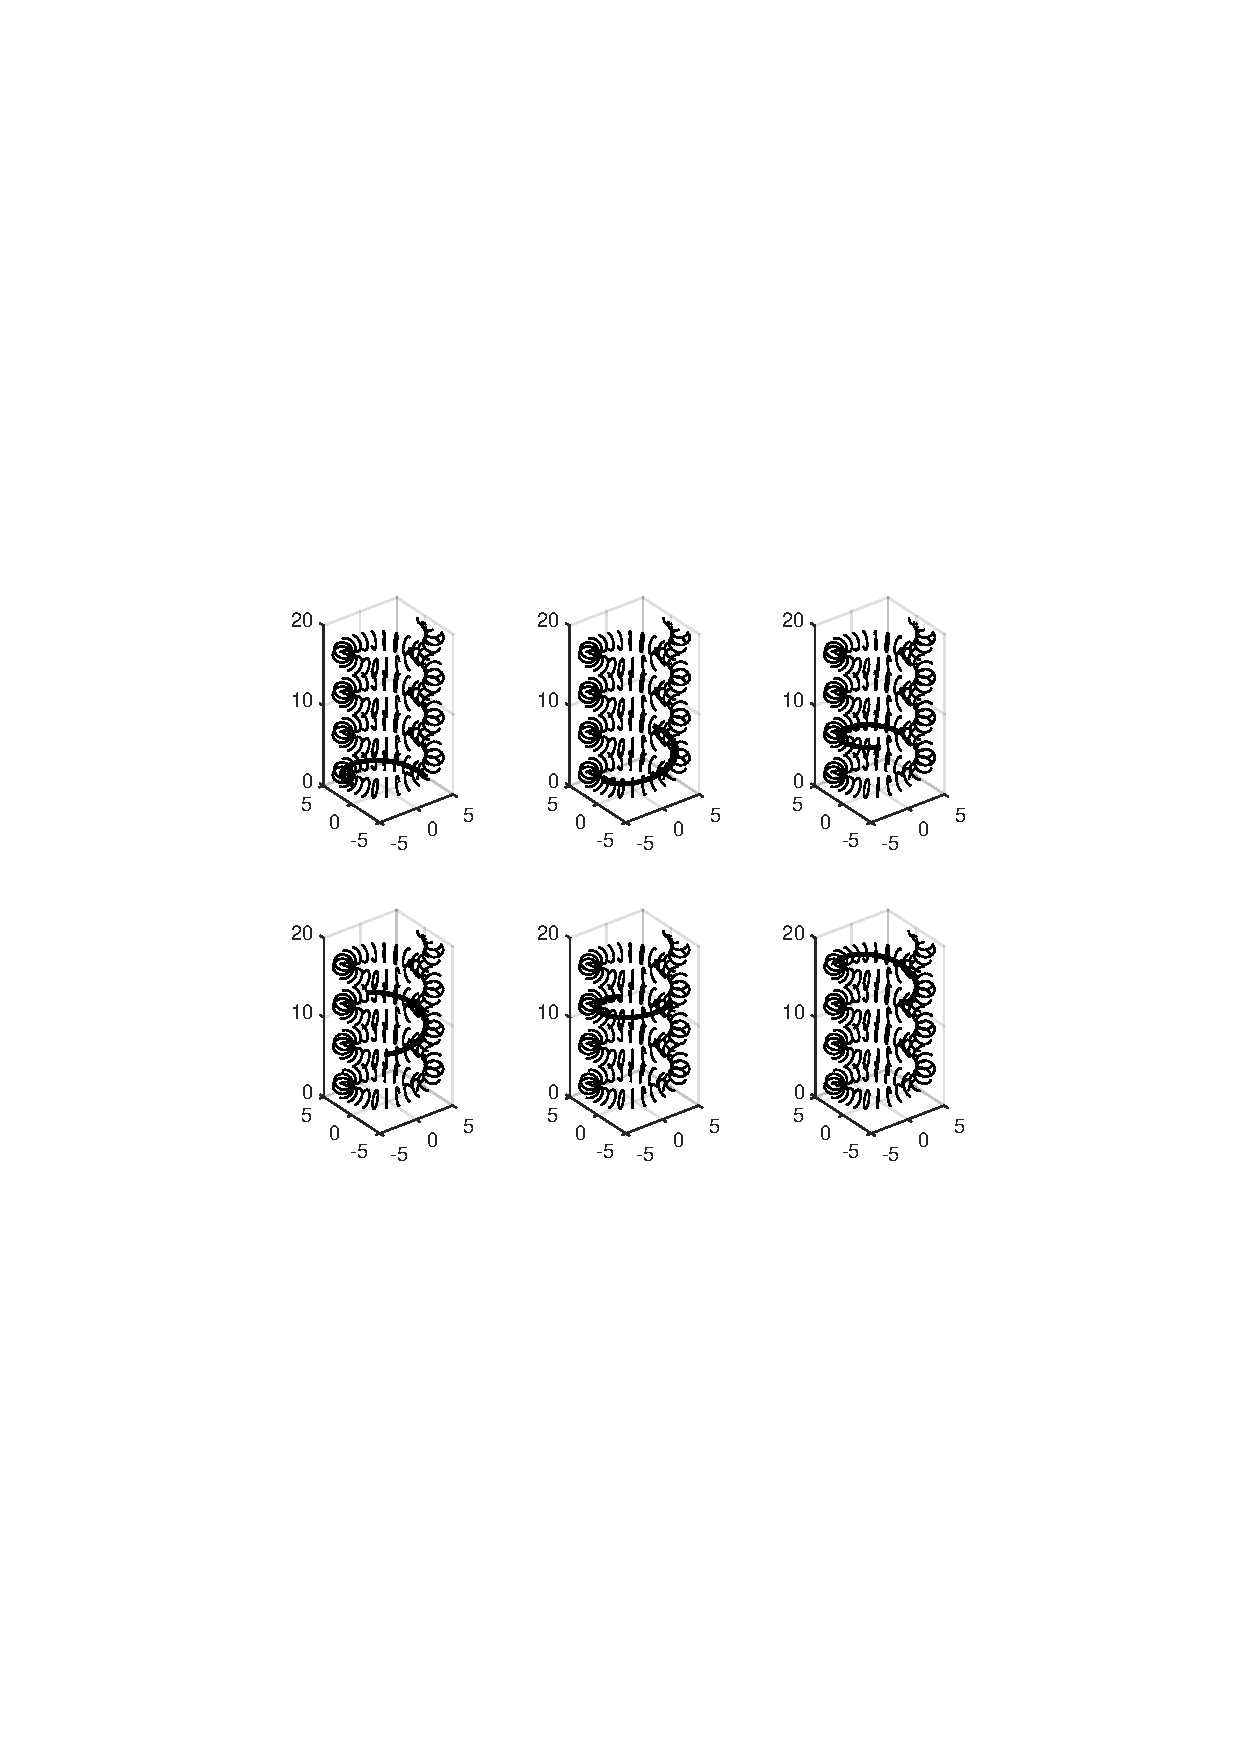
\includegraphics[scale=0.75]{figures/analytduct.pdf}
%\caption{ Motion of hyper-redundant robot through helical duct \label{fig:helicalduct}}
%\end{figure}

\section{Examples and discussion}
\label{sec:Examples}
In this section, we present three practical examples where the above mentioned methods are applied and some discussion on the implementation of the above mentioned algorithms.
\subsection{Examples of motion planning through ducts}

\subsubsection{Motion planning for inspection robots}
One major use of hyper-redundant robots is in inspection of ducts such as industrial pipelines. By approximating the pipe-line as ellipsoids or cylinders, methods mentioned above are made use of, to plan the motion of a hyper-redundant robot through the same. The path is chosen as the medial axis of the duct, which is also the axis of the cylinders which make up the duct. The configuration of hyper-redundant robot for each path-step is calculated and the simulation of resultant motion is shown in \cref{fig:pipelinemotion}.
\begin{figure}[ht!]
    \centering
    \begin{subfigure}{0.31\textwidth}
        \centering
        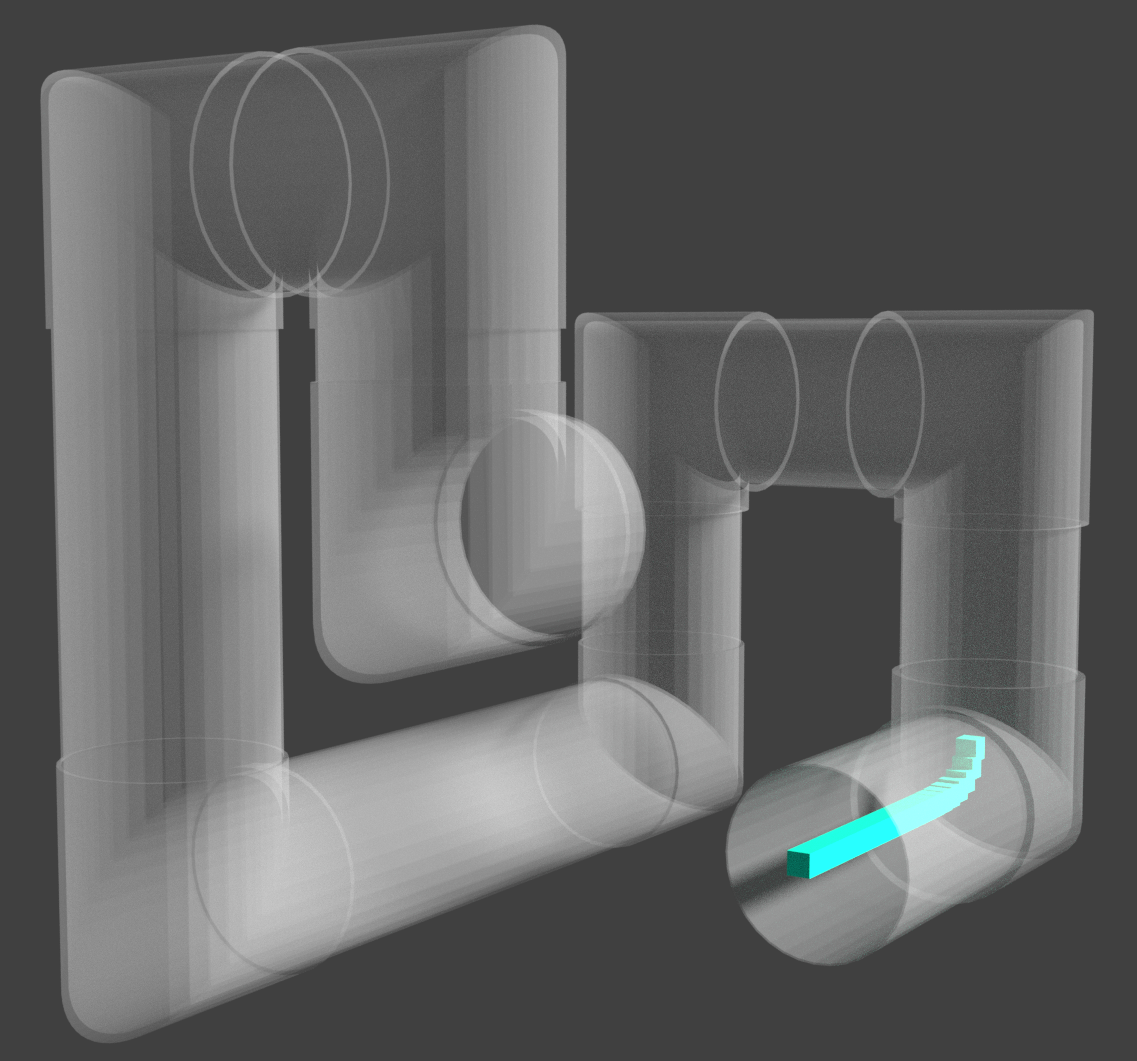
\includegraphics[width=0.8\linewidth]{figures/Pipesnaps/1.png}
   
    \end{subfigure}%
    ~
        \begin{subfigure}{0.31\textwidth}
        \centering
        \includegraphics[width=0.8\linewidth]{figures/Pipesnaps/2.png}
       
    \end{subfigure}%
    ~
        \begin{subfigure}{0.31\textwidth}
        \centering
        \includegraphics[width=0.8\linewidth]{figures/Pipesnaps/3.png}
      
    \end{subfigure}%
    \\~\\
    
       \begin{subfigure}{0.31\textwidth}
        \centering
        
\includegraphics[width=0.8\linewidth]{figures/Pipesnaps/4.png}
       
    \end{subfigure}%
    ~
        \begin{subfigure}{0.31\textwidth}
        \centering
        \includegraphics[width=0.8\linewidth]{figures/Pipesnaps/5.png}
      
    \end{subfigure}%
    ~
        \begin{subfigure}{0.31\textwidth}
        \centering
        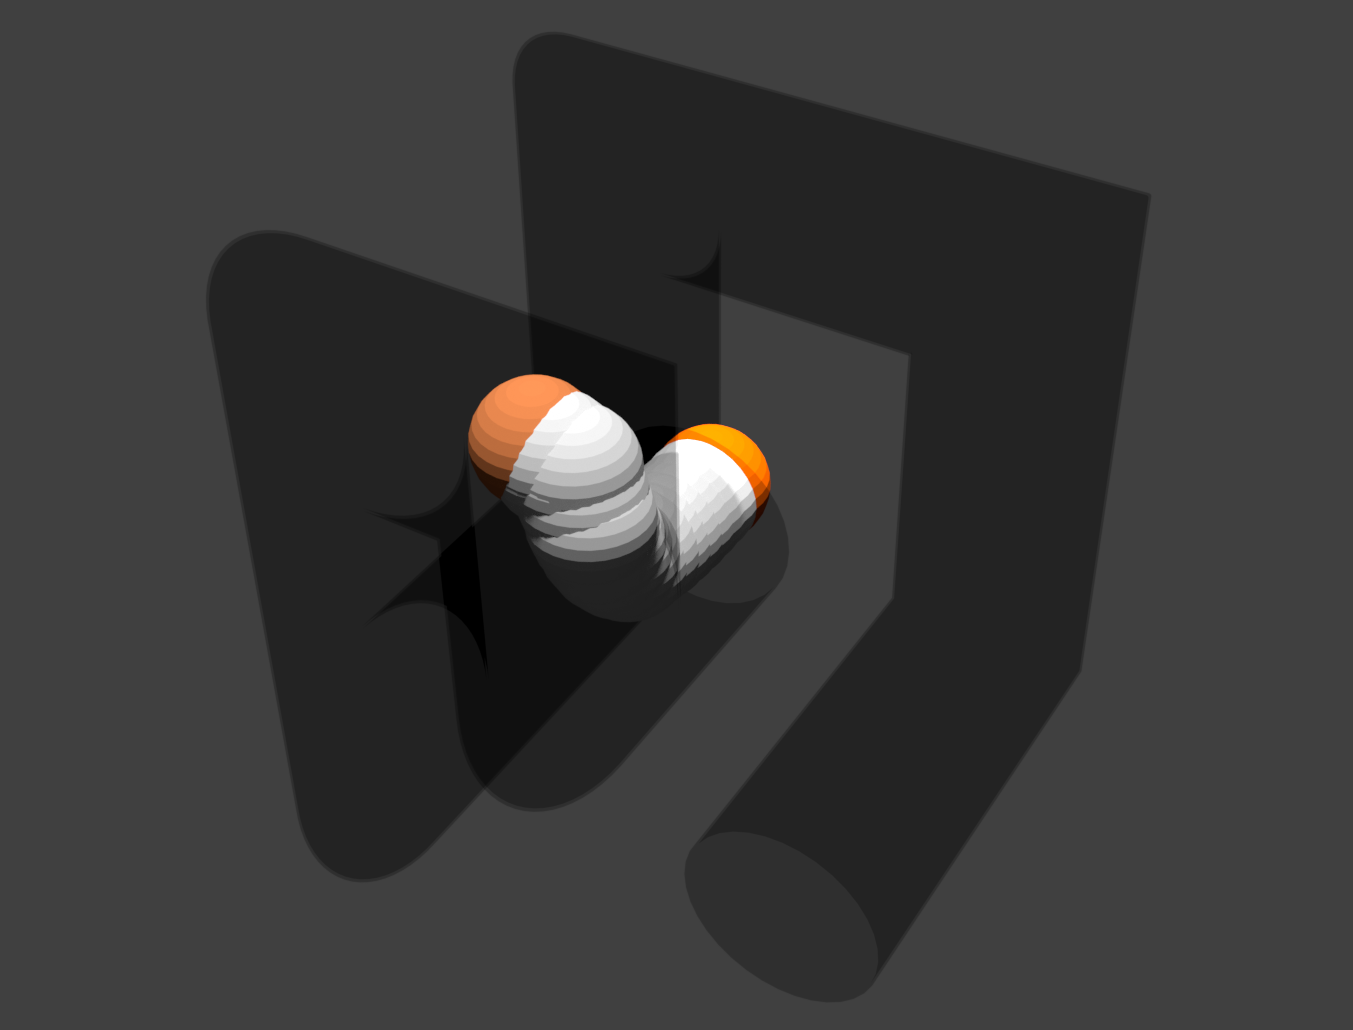
\includegraphics[width=0.8\linewidth]{figures/Pipesnaps/6.png}
        
    \end{subfigure}%
    
    \caption{ Motion of hyper-redundant manipulator through a duct represented as connected cylinders\label{fig:pipelinemotion}}
\end{figure}


\subsubsection{Motion planning through a GI tract}
There has been a growing interest in simulating motion of endoscope through GI tract for developing simulators for endoscopy and for implementing path and motion plans for endoscopic and laparoscopic surgical robots. In this section, we simulate the natural motion of an endoscope through GI tract. For simulation, we use the stereolithographic data of GI tract obtained by processing CT scan data. For demonstration, both the methods presented in [sec] and [sec] are used for approximating the GI tract. In the first method, a collection of points are manually selected from the STL file where super-elliposids are fit based on least square error minimization techniques.  Representation of GI tract as series of super-ellipsoids is shown in [fig19]

\begin{figure}[ht!]
    \centering
    \begin{subfigure}{0.48\textwidth}
        \centering
        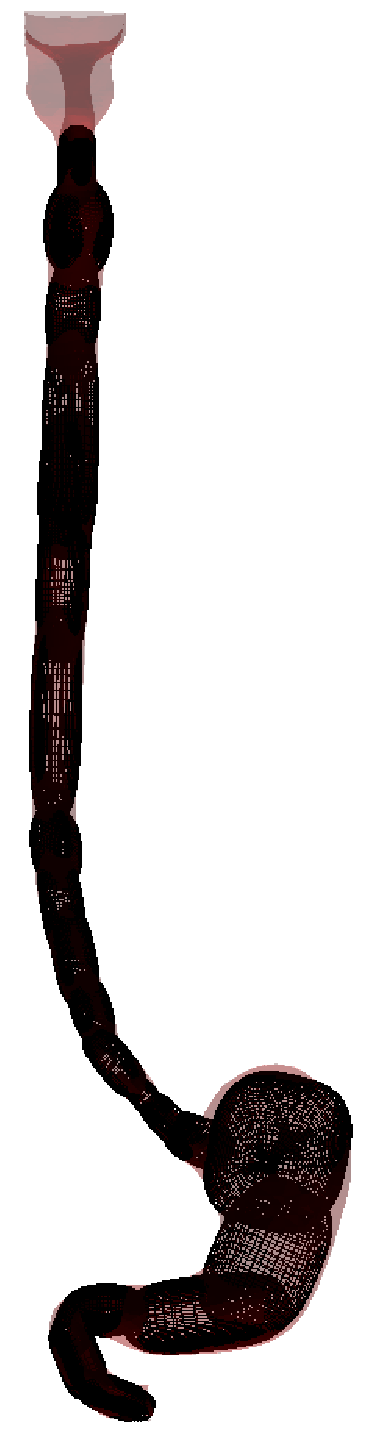
\includegraphics[width=0.25\linewidth]{figures/fig19.pdf}
        \caption{GI tract as collection of super-elliposids \label{fig:GISEs}}
    \end{subfigure}%
    \begin{subfigure}{0.48\textwidth}
        \centering
        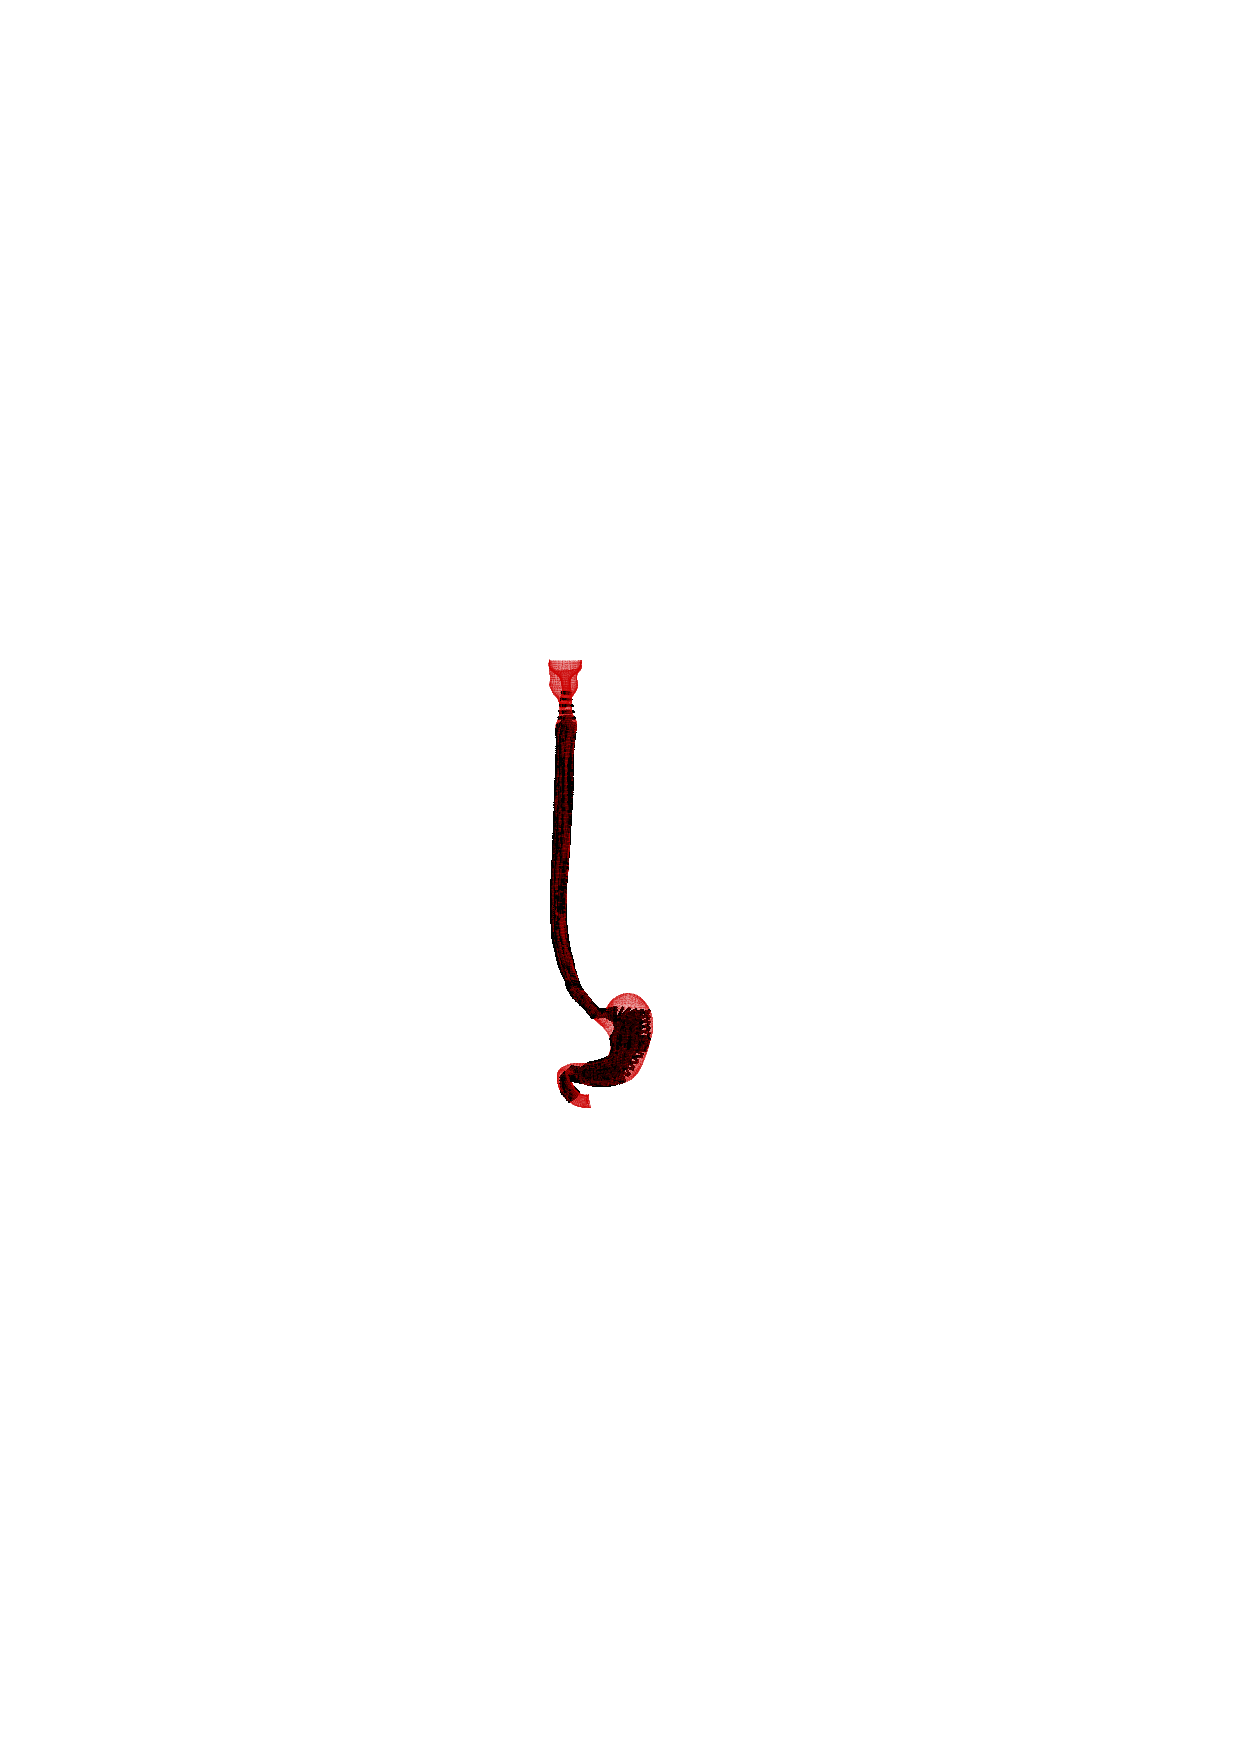
\includegraphics[width=0.25\linewidth]{figures/GIcylfit.pdf}
        \caption{GI tract with connected cylinders\label{fig:GICYs}}
    \end{subfigure}
    \caption{ Representation of GI tract in two methods}
\end{figure}

For representing GI tract as cylinders, we first found out the medial axis of the duct using ??. Then at equal intervals of distance along the medial axis, planes are drawn normal to the same. The collection of points which are in the close proximity of the plane are selected and a circle is fitted on the points using least square error minimization. The parameters so obtained are used for the cylinder equations in [\ref{eq:cylinder}]. Representation of GI tract as a series of connected cylinders is shown in [fig20]

The realistic motion simulation of endoscope through GI tract is shown in [fig21]

\begin{figure}[ht!]
    \centering
    \begin{subfigure}{0.15\textwidth}
        \centering
        \includegraphics[width=0.9\linewidth]{figures/GIsnaps/1.png}
   
    \end{subfigure}%
    ~
       \begin{subfigure}{0.15\textwidth}
        \centering
        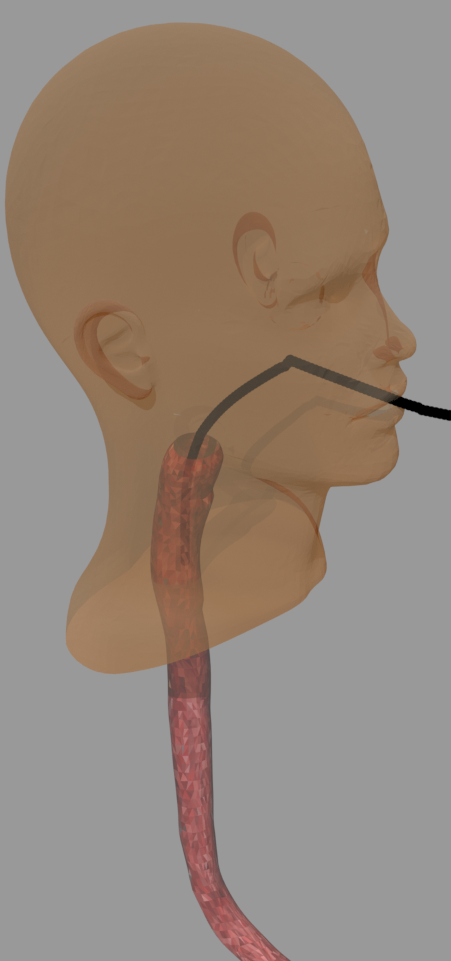
\includegraphics[width=0.9\linewidth]{figures/GIsnaps/2.png}

    \end{subfigure}%
       \begin{subfigure}{0.15\textwidth}
        \centering
        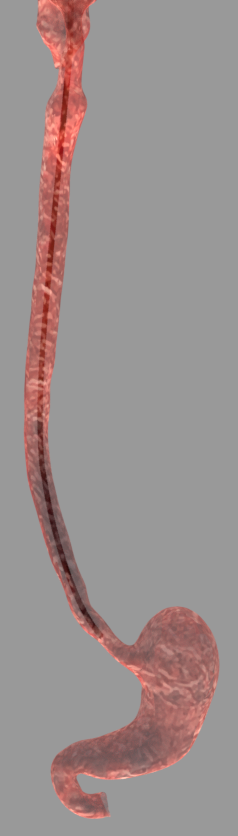
\includegraphics[width=0.75\linewidth]{figures/GIsnaps/3.png}

    \end{subfigure}%
		~   
       \begin{subfigure}{0.15\textwidth}
        \centering
        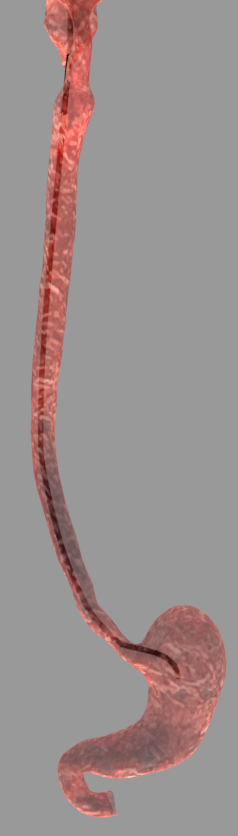
\includegraphics[width=0.75\linewidth]{figures/GIsnaps/4.png}
       
    \end{subfigure}%
    ~
        \begin{subfigure}{0.15\textwidth}
        \centering
        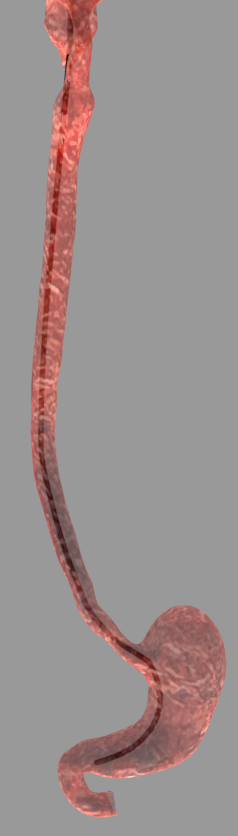
\includegraphics[width=0.75\linewidth]{figures/GIsnaps/5.png}
      
    \end{subfigure}%
    ~
        \begin{subfigure}{0.15\textwidth}
        \centering
        \includegraphics[width=0.75\linewidth]{figures/GIsnaps/6.png}
        
    \end{subfigure}%
    
    \caption{ Motion of endoscope through GI tract}
\end{figure}

\subsubsection{Motion planning for search and rescue operations}
Exploring a cluttered environment-- such as in an earthquake hit zone is one of the major applications that necessitates the use of hyper-redundant manipulators. In this example, we show how the proposed algorithms can be effectively used in such applications. With reference to [fig ??], the objective of the hyper-redundant manipulator, consisting of 20 links is to 1) enter the scene through the hole in the outer wall, 2) Pass through the vent to get inside the room, 3) Explore the objects 1,2 and 3 located inside the blue region and 4) Exit without colliding with the complex shapes given by objects 4 and 5. Here, the exploration problem is effectively tackled using the following constraints added to the optimization problem (refer Fig ??): 1) An ellipsoid of the size of the hole located in the outer wall 2) collection of cylindrical ducts to represent the vent, 3) STL models for the objects 1,2 and 3 and 4) Ellipsoid at the last bend in the path to avoid collision with the complex shapes of objects 4 and 5 (orange color). It is easy to see that the geometry based global motion planning techniques for obstacle avoidance existing in literature will entail a very involving problem formulation [ananthanarayanan]. While using the methods proposed in this paper, the problem can be addressed with only 6 constraints. The six constraints in this case are actively selected so that they become active only when the position of the head is in the vicinity of the objects/ shapes. Figure [??] shown the simulated results for the motion of manipulator along a chosen path. 

\begin{figure}[h!]
\centering
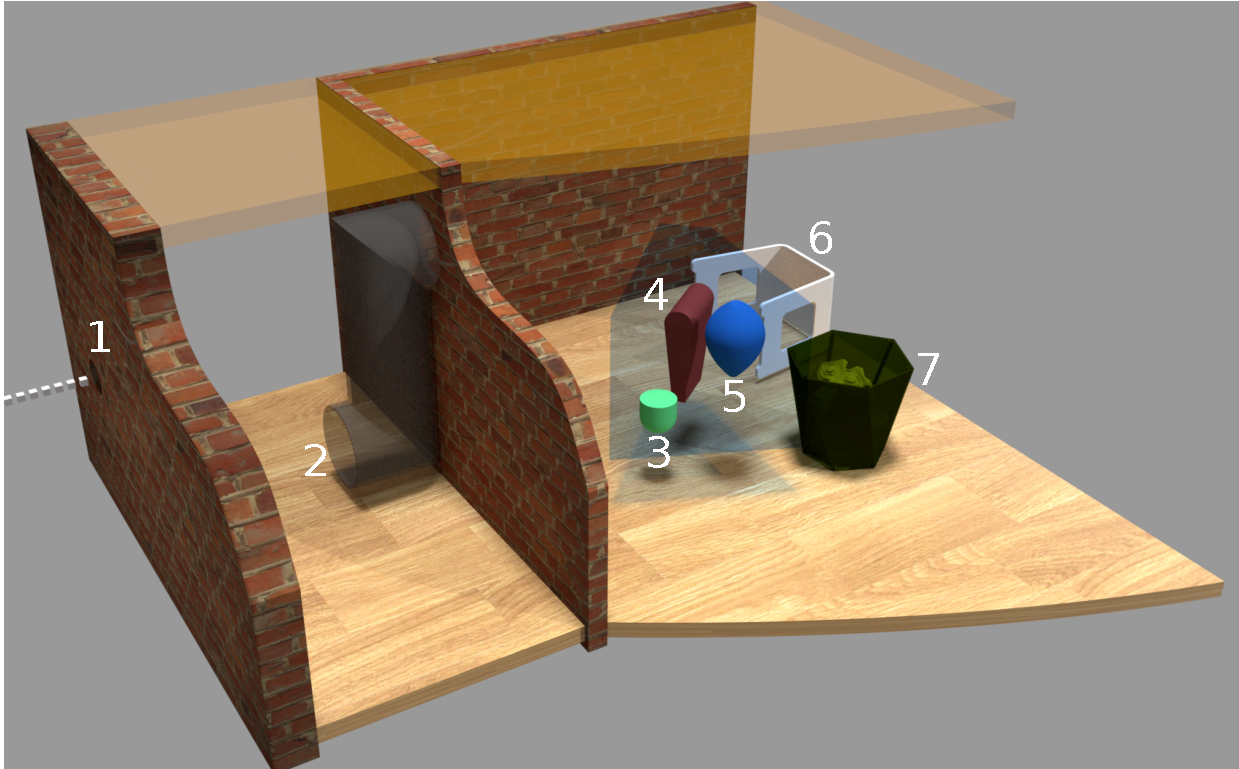
\includegraphics[scale=0.65]{figures/figscene.pdf}
\caption{ Scene of search and rescue problem \label{fig:scene}}
\end{figure}


\begin{figure}[ht!]
    \centering
    \begin{subfigure}{0.3\textwidth}
        \centering
        \includegraphics[width=1\linewidth]{figures/Sceneshots/1.png}
   
    \end{subfigure}%
    ~
        \begin{subfigure}{0.3\textwidth}
        \centering
        \includegraphics[width=1\linewidth]{figures/Sceneshots/2.png}
       
    \end{subfigure}
        ~
        \begin{subfigure}{0.3\textwidth}
        \centering
        \includegraphics[width=1\linewidth]{figures/Sceneshots/3.png}
       
    \end{subfigure}%\\
\\
~\\
        \begin{subfigure}{0.3\textwidth}
        \centering
        
\includegraphics[width=1\linewidth]{figures/Sceneshots/4.png}

    \end{subfigure}%
		~   
       \begin{subfigure}{0.3\textwidth}
        \centering
        \includegraphics[width=1\linewidth]{figures/Sceneshots/5.png}
           \end{subfigure}
               ~
        \begin{subfigure}{0.3\textwidth}
        \centering
        \includegraphics[width=1\linewidth]{figures/Sceneshots/6.png}
       
    \end{subfigure}
    \caption{ Motion of hyper-redundant robot in confined spaces ?? Fig will be edited??}
\end{figure}

\subsection{Computational complexity of the proposed scheme} \label{sc:Complexity}

An important aspect of the formulations described in the current work was to show that the formulation and implementation of motion planning problem using tractrix is intuitive and has a broad scope of application. In concurrence to that theme, in this section, we attempt to analyze the worst case computational complexity of such an implementation to show that the current work has potential for real time application in actual problems. We begin by reviewing some mathematical concepts, after Boyd[opt book], to be used in the following discussion.\\
\indent \textit{Self Concordance}: A convex function $f: \mathbb{R} \to \mathbb{R}$ is \textit{self-concordant} if $|f'''(x)|\leq 2f''(x)^{3/2}$ for all $x \in \textbf{dom}f$. It can be shown that the Eucledian norm and linear functions are self concordant.\\
%\indent \textit{The big-O notation} ($\mathcal{O}$): For two functions $f,~g: \mathbb{N}\to \mathbb{R}^+$, the function $g$ is an asymptotically upper bound for $f$, denoted by $f(n)~\epsilon~ \mathcal{O}(g(n))$, if there exists a constant $c>0$ and $n_0\epsilon \mathbb{N}$ such that $\forall n> n_0$, $f(n)\leq cg(n)$.  \\
\indent \textit{Feasible set}: For an optimization problem with constraints $f_i(\textbf{x})\leq 0$ and $h_j(\textbf{x})=0$, for $i=1,2,...,n$ and $j=1,2,...,m$, the feasible set is $\mathcal{S}=\cap_{i=1}^n~\textbf{dom}(f_i\leq0)\cap\cap_{j=1}^m~\textbf{dom}(h_j=0)$. For all our problems, $\mathcal{S} $ is a subset of the real space $\mathbb{R}$ of dimension 2 or 3.\\
\indent \textit{Slater's condition}: Slater's conditions of constraint qualification hold when there exists an $\textbf{x}~ \in \mathcal{S}$, a strictly feasible point,  such that all the inequality conditions and equality conditions are satisfied\footnote{We resort to a slight misuse of notation for brevity. For a more complete treatment, one may refer to Chapter 5 of the book by Boyd and Vandenberghe [Boyd book].}. This would, in general, mean that strong duality would hold and at the optimum point, the primal and dual problem would have the same solutions.\\
With these, we move on to our topic of complexity analysis. In \cref{sc:optimization} we have discussed that the problem as presented in \cref{eq:Opt_prob_main} is not  convex due to the non-linear equality constraint guaranteeing the length of a link is constant at all times. We get around by replacing the non-linear equality constraint by it's affine equivalent-- a first order approximation of the constraint about a feasible point $\textbf{x}^* \in \mathcal{S}$, and a trust region constraint as shown in problem in \cref{eq:Opt_prob_mod}. It is imperative for the trust region radius to be small-- in our implementation, we have chosen the trust region radius $\epsilon_T$ to be about 6 orders of magnitude smaller than the smallest dimension of $\mathcal{S}$. In \cref{eq:Opt_prob_mod}, $\nabla_{\textbf{x}_t}$ is the gradient of the objective function. 
\begin{align}\label{eq:Opt_prob_mod}
 \argmin_{\textbf{x}_t} & ~g(\textbf{x}_t): \vert \vert \textbf{x}_t-\textbf{X}_t\vert \vert\\
\text{Subject to}~: &~ g(\textbf{x}^*)-\nabla_{\textbf{x}_t}g(\textbf{x}^*) (\textbf{x}_t-\textbf{x}^*) =0\nonumber\\ 
					& | \textbf{x}^*-\textbf{x}_t| \preceq  \epsilon_T \nonumber\\
					& C_{ineq}: f(x) \preceq 0 \nonumber
\end{align}

We can rewrite \cref{eq:Opt_prob_mod} as a standard nonlinear program with the objective function $g$, all the $'m'$ constraints $\textbf{f}$ and $\textbf{s}$, a vector of $m\times 1$ slack variables as 
\begin{align} \label{eq:standard_non_lin_prog}
\argmin_{\textbf{x}_t} ~& g(\textbf{x}_t) \\
\text{Subject to: }~ & \textbf{f}(\textbf{x}_t)+\textbf{s} =0 \nonumber\\
& \textbf{s}\succeq 0\nonumber
\end{align} 
We also observe that the problem in \cref{eq:Opt_prob_mod} corresponding to the implementations studied so far, is actually a minimum norm problem with either polyhedral (or polygonal in 2D)  or super-quadric (or super-elliptic) constraints. As all of the constraints qualify Slater's condition, we conclude that strong duality holds for all  versions of the problem studied in the current work. We choose a interior point method to solve the nonlinear programming problem at hand and by reformulating \cref{eq:standard_non_lin_prog} as a barrier problem with barrier parmeter $\mu$. The KKT necessary and sufficient conditions for the given problem is given in \cref{eq:KKT_system}.
\begin{align}\label{eq:KKT_system}
\nabla_{\textbf{x}_t}g(\textbf{x}_t)+\nabla_{\textbf{x}_t}\textbf{f}(\textbf{x}_t)^T \vec{\lambda} =0 \nonumber \\
\textbf{f}(\textbf{x}_t)+\textbf{s}=0 \\
\textbf{L}\textbf{S}-\mu \vec{e}=0 \nonumber
\end{align}
In \cref{eq:KKT_system}, $\textbf{L}$ is the $m \times m$ diagonal matrix of the Lagrange multipliers ($\vec{\lambda}$), $\textbf{S }$ is the $m \times m$ diagonal matrix of the slack variables $\textbf{s}$ and $\textbf{e}$ is a $m\times 1$ vector of ones. The above system represents $2m+1$ equations in $2m+1$ variables and is known as the KKT system. While using an interior point methods, the computation times depend on two principal factors-- the number of Newton steps required to converge and the complexity of each Newton step i.e. total amount of computation required in solving \cref{eq:KKT_system} to obtain the Newton direction. For our case with  a self-concordant log barrier and polyhedral constraints, which are by default self-concordant, we can conclude that the total number of Newton steps are of the order of $\sqrt{m}+c$ where $c$ is a integer. In case of our problems, we actually observed this phenomenon where, for a 2D case the total number of iterations were about 10, for $m=6$ for 4 linear constraints defining $\mathcal{S}$ and 2 trust region constraints.\\
\Cref{eq:KKT_system} can be linearized, and solved (for a 3D case) to obtain the Newton direction as
\begin{align}\label{eq:Lin_KKT}
\left(\begin{array}{ccc}
 A_{3\times3} & B^T_{m\times 3} & 0_{3\times m} \\ 
B_{3\times m}  & 0_{m\times m} & I_{m\times m} \\ 
0_{6\times m} & \textbf{S} & \textbf{L}
\end{array}  \right) \left( \begin{array}{c}
\triangle\ x \\ 
\triangle \lambda \\ 
 \triangle s
\end{array}  \right) = \left( \begin{array}{c}
-\textbf{F}_1 \\ 
-\textbf{F}_2 \\ 
-\textbf{F}_3
\end{array}  \right) 
\end{align}
where, $\textbf{A}=\nabla_{\textbf{x}_t}^2g(\textbf{x}_t)+\sum\limits_{i=1}^{m}\nabla_{\textbf{x}_t}^2\lambda_if_i(\textbf{x}_t)$ is a $3\times3$ symmetric matrix, $B=\nabla_{\textbf{x}_t}\textbf{f}(\textbf{x}_t)$ is a $m\times3$ matrix of the gradient of the $m$ constraint functions, and $\textbf{F}_1$, $\textbf{F}_2$, and $\textbf{F}_3$ are the left hand sides of \cref{eq:KKT_system}. Following [put nilanjan's ieee tro paper] we can obtain the Newton directions as:
\begin{align}\label{eq:Newton-dir}
&\triangle \textbf{x}_t=\textbf{G}^{-1}(-\textbf{F}_1-\textbf{B}^T(\textbf{S}^{-1}\textbf{L})(\textbf{F}_2+\textbf{L}^{-1}\textbf{F}_3)) \nonumber \\
&\triangle\lambda=(\textbf{S}^{-1}\textbf{L})(\textbf{B}\triangle \textbf{x}_t -\textbf{F}_2+\textbf{L}^{-1}\textbf{F}_3)\\
&\triangle s = -\textbf{L}^{-1}(\textbf{F}_3+\textbf{S}\triangle \lambda) \nonumber
\end{align}
 Where, $\textbf{G}= \textbf{A}+\textbf{B}^T(\textbf{S}^{-1}\textbf{L})\textbf{B}$, a $3\times3$ matrix (for a 3D case) which can be inverted symbolically, also, $\textbf{S}$ and $\textbf{L}$ are diagonal matrices so their inverse can be calculated in linear time ($\mathcal{O}(m)$). Overall, the asymptotic complexity of solving \cref{eq:Newton-dir} is $\mathcal{O}(m^3)$ as the calculation of $ G^{-1},~ \triangle x$ and $\triangle \lambda$ are $\mathcal{O}(m^3)$. This would result in a total asymptotic complexity of the implementation to be $\mathcal{O}(m^{3.5})$. However, the computation time of an iteration doesn't depend on the number of links of the hyper-redundant robot or the step size path, hence the proposed method is linear in these. This is observed from \cref{fig:path_complexity}. As discussed in \cref{sc:duct_as_STL}, in our implementation of the motion planning problem inside a polyhedral domain, we use a separate algorithm to determine whether to use the constraints of the form $[\mathbf{A}]_{m\times 3}\mathbf{x}_t+\mathbf{B}_{m\times 1}\leq 0$ in \cref{eq:STLeqs}. \Cref{alg:in_hull} discusses an $\mathcal{O}(m)$ algorithm to do the same in case of a polyhedron with $ m $ faces. Therefore, the total asymptotic complexity of our implementation should be about $\mathcal{O}(m^{1.5})$. \Cref{fig:face_complexity} shows that actual complexity implementation of our algorithm scales as $(m^{1.43})$, with room for further improvement\footnote{Computation times in \cref{fig:complexity} was obtained using the `tic-toc' function in MatlabR2016b running on a workstation with dual 8 core Intel XEON (2.1GHz), 32 GB RAM and Windows 10. The constant term in the fit equation shown in \cref{fig:face_complexity} signifies the time required to compute the free tractrix problem given by \cref{eq:Opt_prob_main}}. Furthermore, the formulations involving parametric shapes (super ellipses and super ellipsoids) are even faster because the classification of a point with respect to the domain is available as a closed form expression. It may also be noted that this analysis is not applicable to cylinders since they require iterative methods to solve the in-out classifier.

To summarize, three methods to represent 3D ducts are discussed in the previous section which can be chosen based on the computational time and required modelling effort. In the first method of representing ducts by a collection of ellipsoids, modelling time is significant as a separate utility is required to identify the points on surface and to fit the ellipsoids on the data points. However, the solution method is quite fast due to the availability of a closed form function for the in-out classification. The second method of fitting cylinders also involve significant amount of pre-processing to identify cylinders that fit the duct. The implementation time is also high due to the non-analytical nature of the in-out classifier. However, the provision of having a constant clearance from the wall makes it particularly attractive for formulating motion plans for which the thickness of the robot has to be taken into account. Finally, the method of using convex polyhedra to represent ducts requires the least pre-processing time, and is easy to implement with the worst case complexity of $\mathcal{O}(m^{1.5})$.

\begin{figure}
\centering
\begin{subfigure}{0.48\textwidth}
\centering
 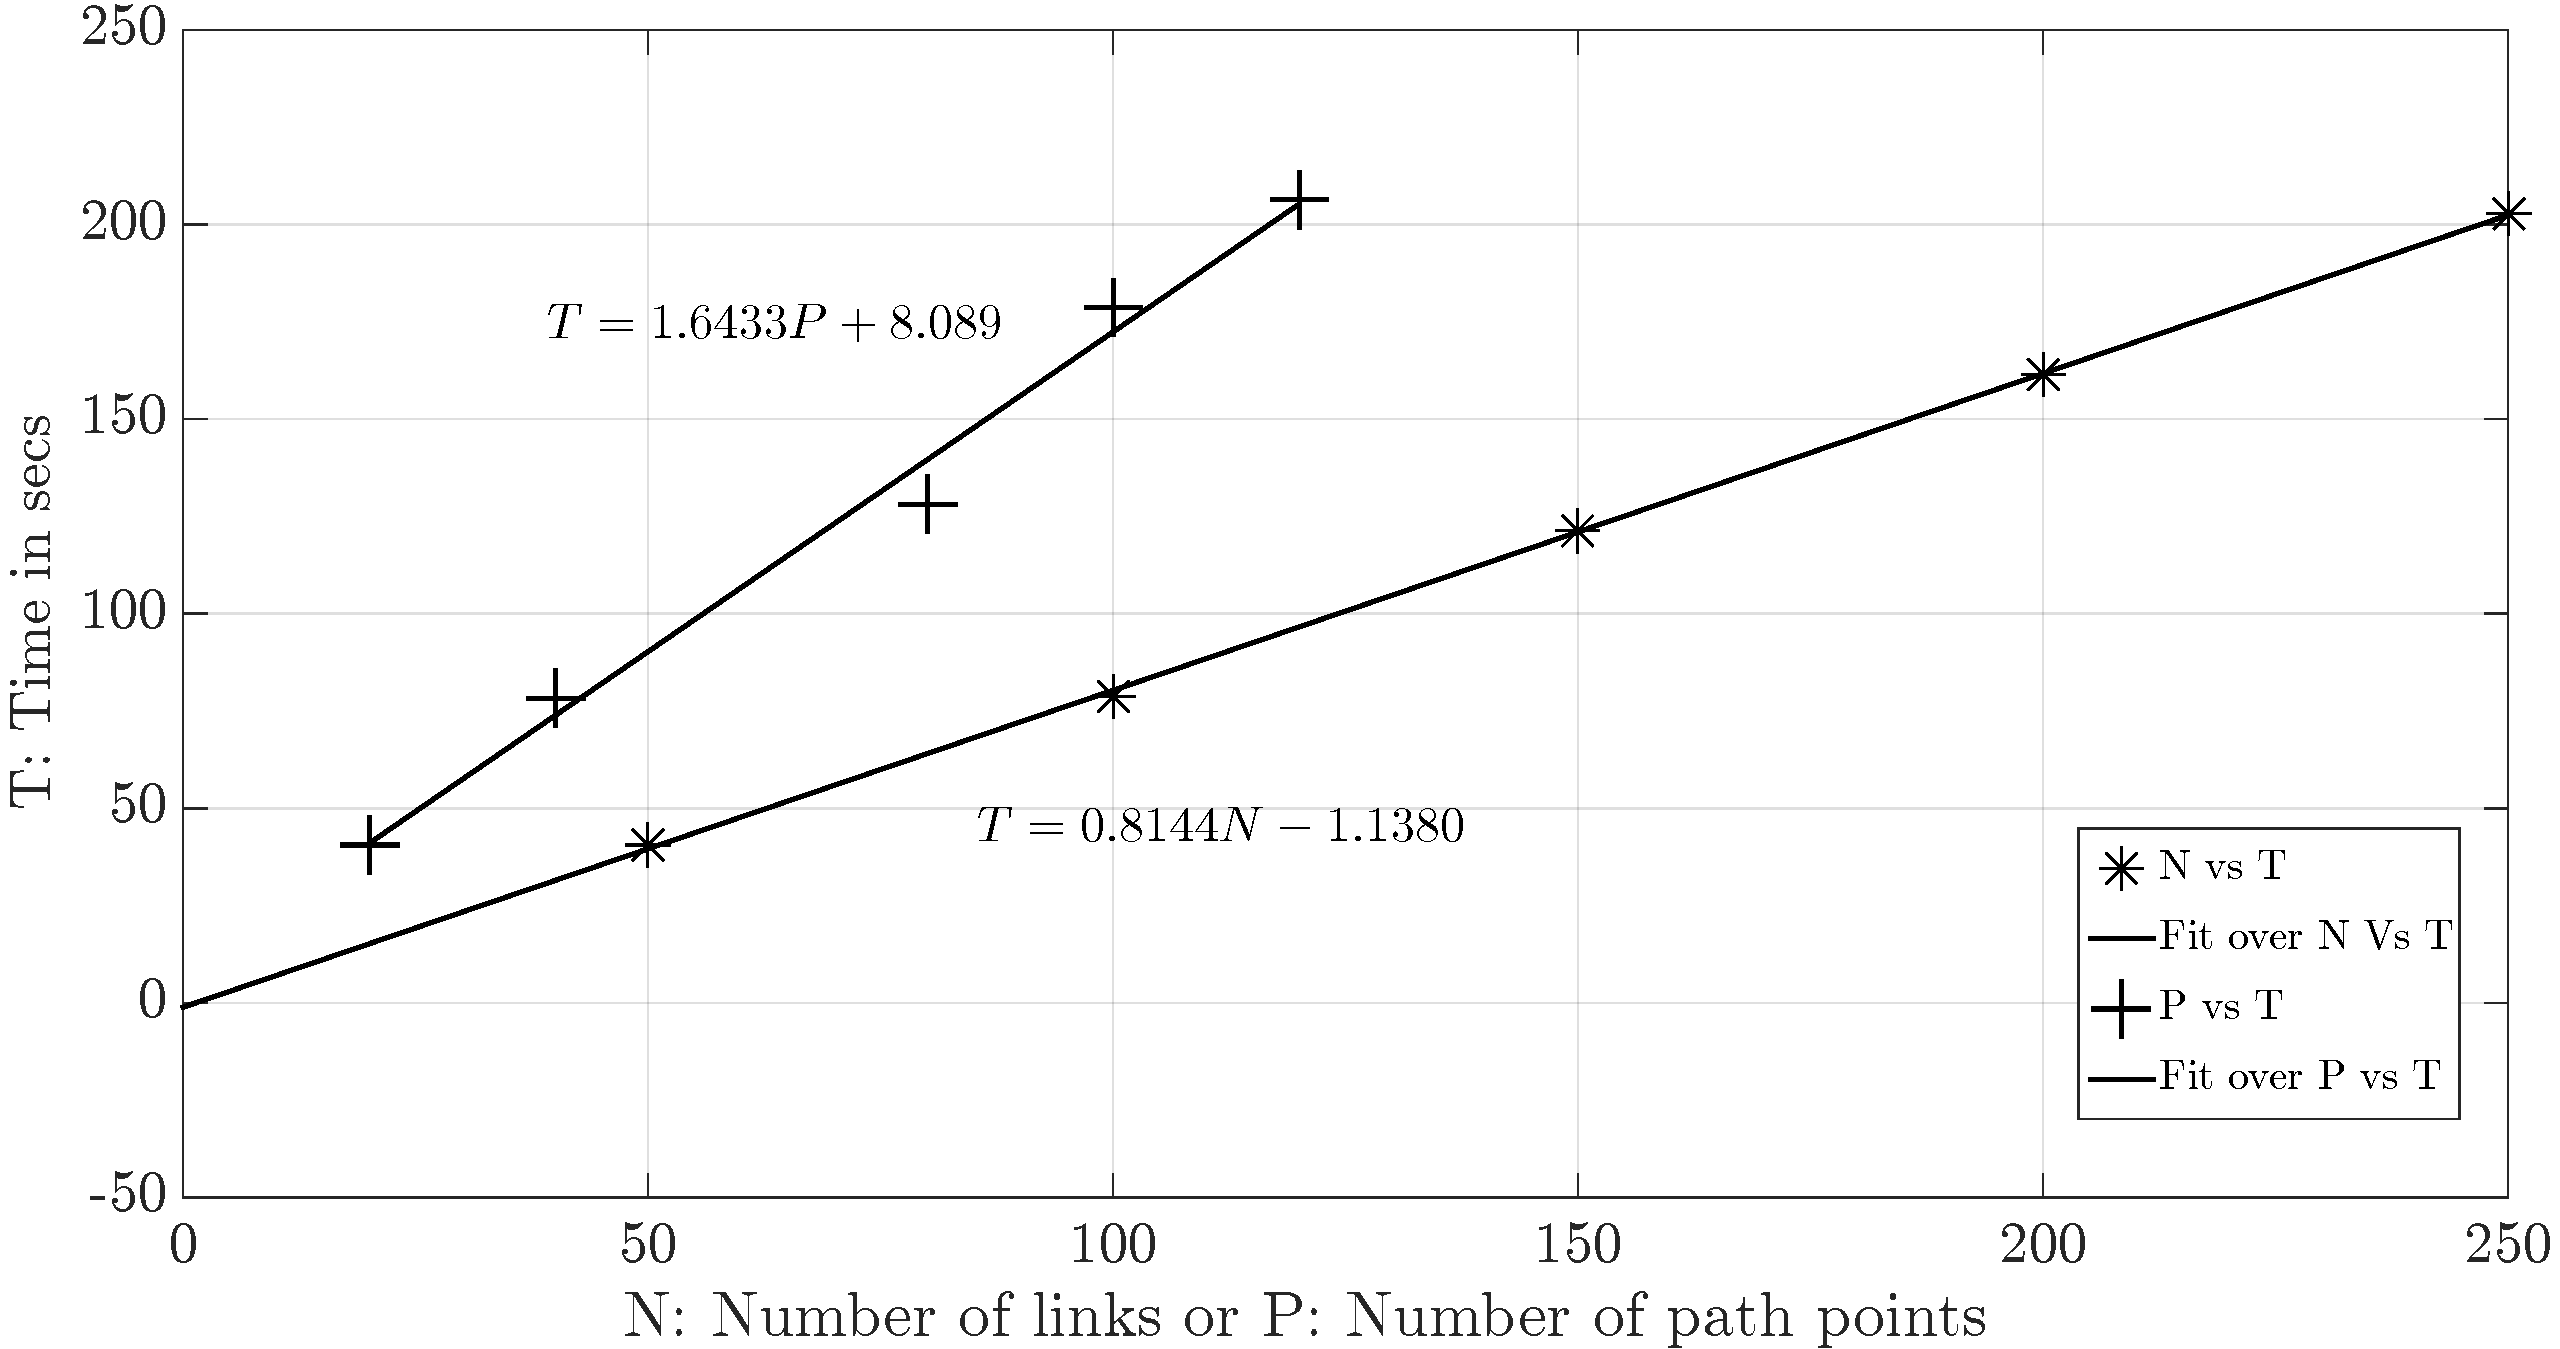
\includegraphics[width=\linewidth]{figures/Path_and_link_complexity.pdf}
\caption{Our implementation is time-linear in number of path points and link numbers}
\label{fig:path_complexity}
\end{subfigure}%
\begin{subfigure}{0.48\textwidth}
\centering
 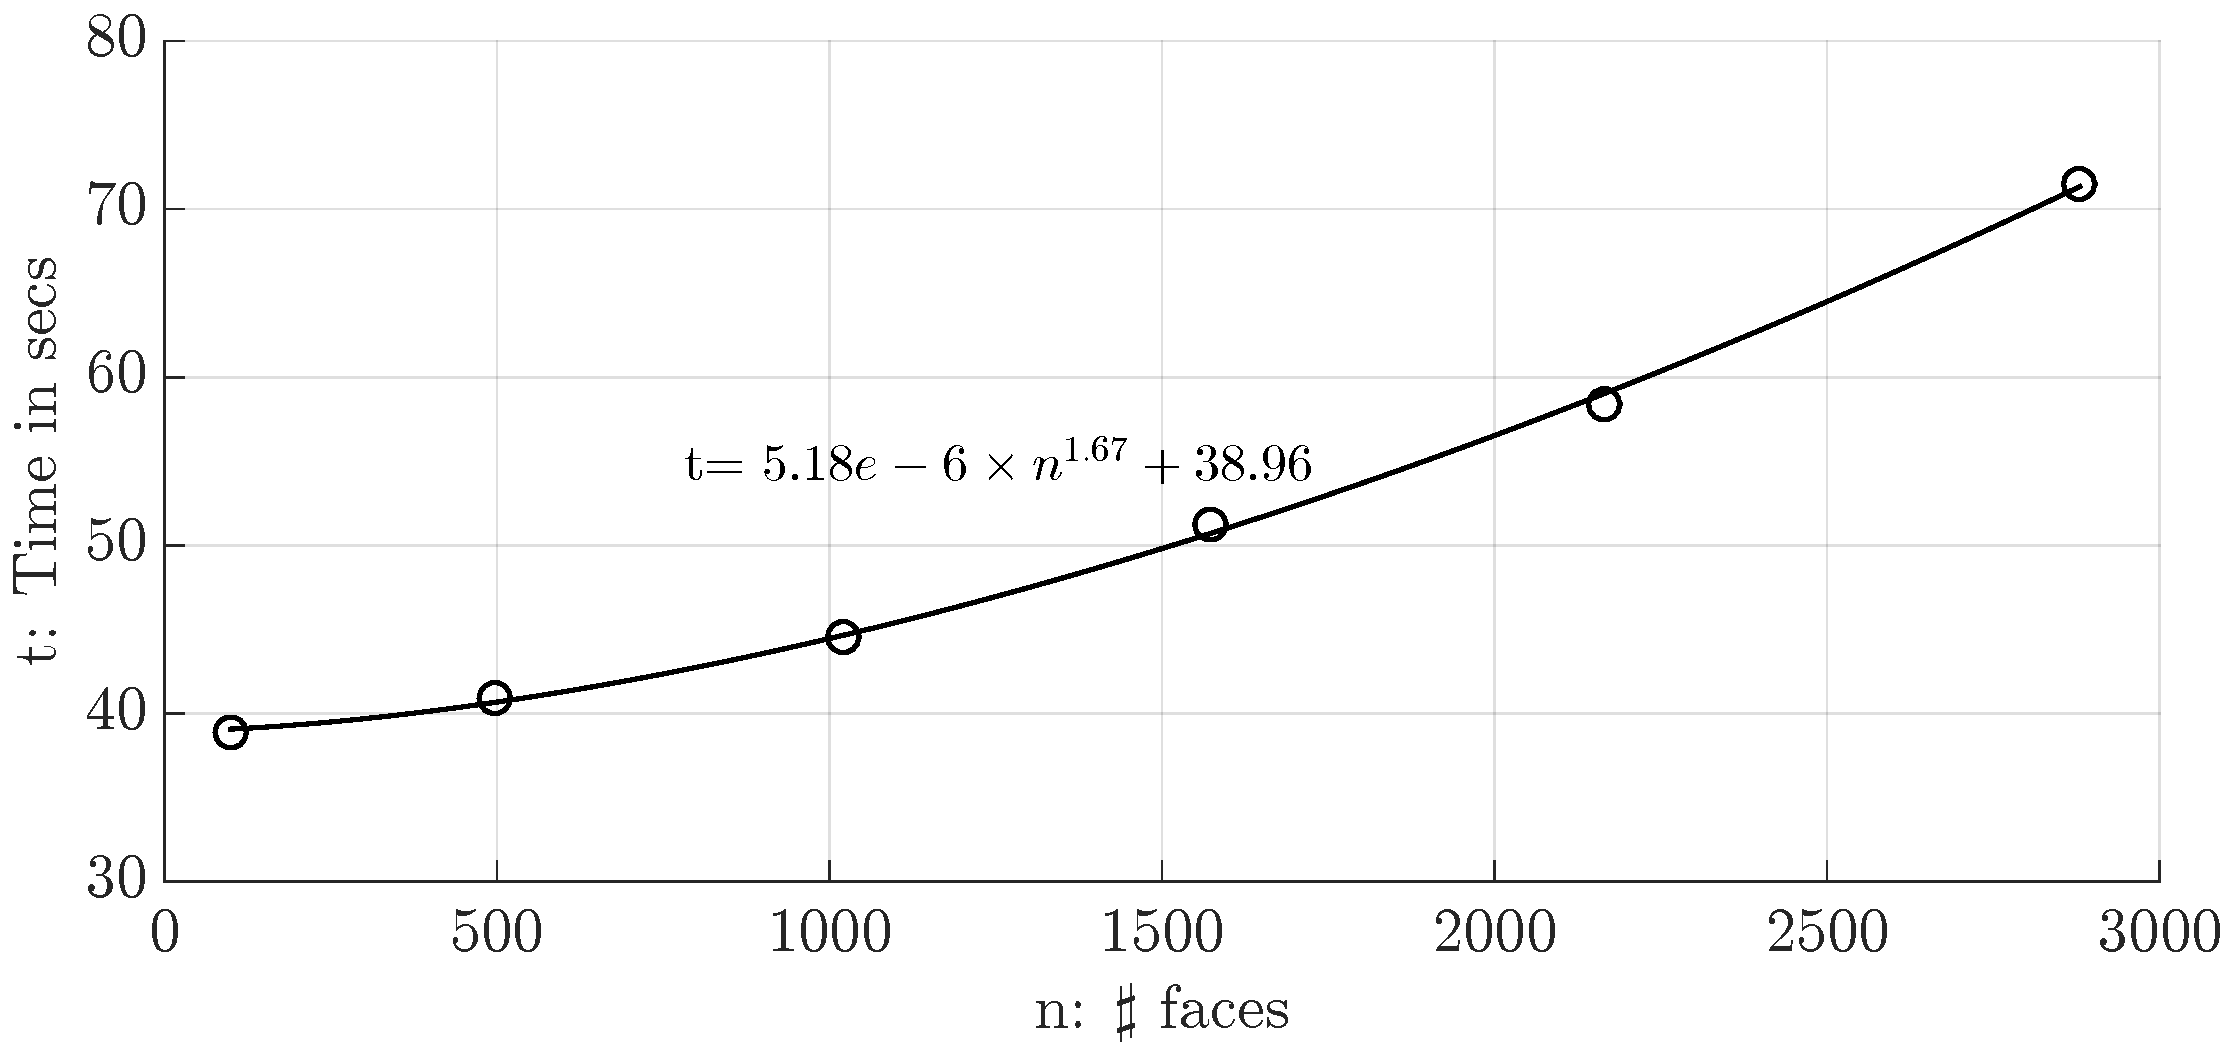
\includegraphics[width=1.1\linewidth]{figures/face_complexity.pdf}
\caption{Our implementation scales as $(m^{1.43})$ }
\label{fig:face_complexity}
\end{subfigure}%
\caption{ Complexity of our implementations}
\label{fig:complexity}
\end{figure}
 
\subsection{Limitations of the tractrix based scheme}
In spite of the certain advantages regarding formulation and computational aspects of the tractrix based motion planning approach, there are a few limitations which are of importance.\\
The ducts represented by analytical curves and cylinders would require an in-out classifier to demarcate the feasible space of the posed optimization problem. Often, this would involve numerical formulations which are quite computationally involving.\\
It can be seen that a given hyper-redundant robot with a particular link length will not be able to negotiate a path with a ``very low" curvature. This is shown in \cref{fig:not_traversable}. In \cref{fig:not_traversable}, the points 1,2,...,8 denote the coordinates of $\textbf{x}_h$ across successive iterations. From iteration 6 onwards, the constraints demarcating the feasible space $\mathcal{S}$ and the one guaranteeing a constant link length cannot be simultaneously satisfied unless the tail $\textbf{x}_t$ (the result of \cref{eq:Opt_prob_main}), backtracks its own path. Soon after, the optimization problem stops as the link seems to be ``locked" at the trough of $\zeta(u)$\footnote{In backbone curve approach, this problem is addressed, but with the cost of very large displacement of the tail point.}. In this section we want to quantify the locking effect. To this end, we borrow the concept of ``traversability" from literature on wheeled mobile robots (see e.g. Nilanjan's JMD paper). A curve $\zeta(u)$ is traversable by a circle $C_i$, $C_i: \left(\begin{array}{c} R_i\cos(v) \\ R_i\sin(v) \end{array}\right), ~ 0 \leq v\leq2\pi $  if $C_i$ can roll over the curve $\zeta(u)$ while maintaining ``only one" point of contact at all times. Traversibility for planar curves can be described by the relative curvature $\kappa_R$ of the circle and the curve at the point of contact. For a planar curve and a circle of radius $R_i$, the relative curvature can be given as \[\kappa_R=\dfrac{\zeta_{uu}}{(1+\zeta_u^2)^{3/2}}-\dfrac{1}{R_i}\] A curve is traversable if the relative curvature is greater than 0, just traversable if it is equal to zero and not traversable if it is negative. This is explained in \cref{fig:is_traversable}. This concept would generalize to traversable surfaces when the minimum of the two eigenvalues of the relative curvature matrix\footnote{The relative curvature matrix of a parametric surface ${S}(u,v): \mathbb{S}^2\to \mathbb{R}^3$ and a sphere of radius R at the point of contact $P = \mathcal{S}(u^*,v^*)$ and on the Gaussian frame attached to the sphere(or $ S $) at P is given as: $\kappa_R\vert_P=\left[\begin{array}{cc}
	{S}_u.{S}_u-1/R & {S}_u.{S}_v \\ 
	{S}_u.{S}_v & {S}_v.{S}_v-1/R
	\end{array}\right]_{u^*,v^*} $} is positive for traversability or vice versa.
Based on this result, we hypothesize that if curve is traversable by a circle of diameter $D_i$, then a hyper-redundant robot of link length $D_i$ can move below the curve without intersecting the curve as shown in \cref{fig:largest_link}. This would also give us an idea about the largest link length that can be used in a hyper-redundant robot traversing a given duct. This concept can also be extended to tessellated surfaces with information about the principal curvatures of the surface at a point (e.g. see the work by Meyer et al. [??]). 
\begin{figure}[ht!]
	\centering
		\begin{subfigure}{0.31\textwidth}
		\centering
		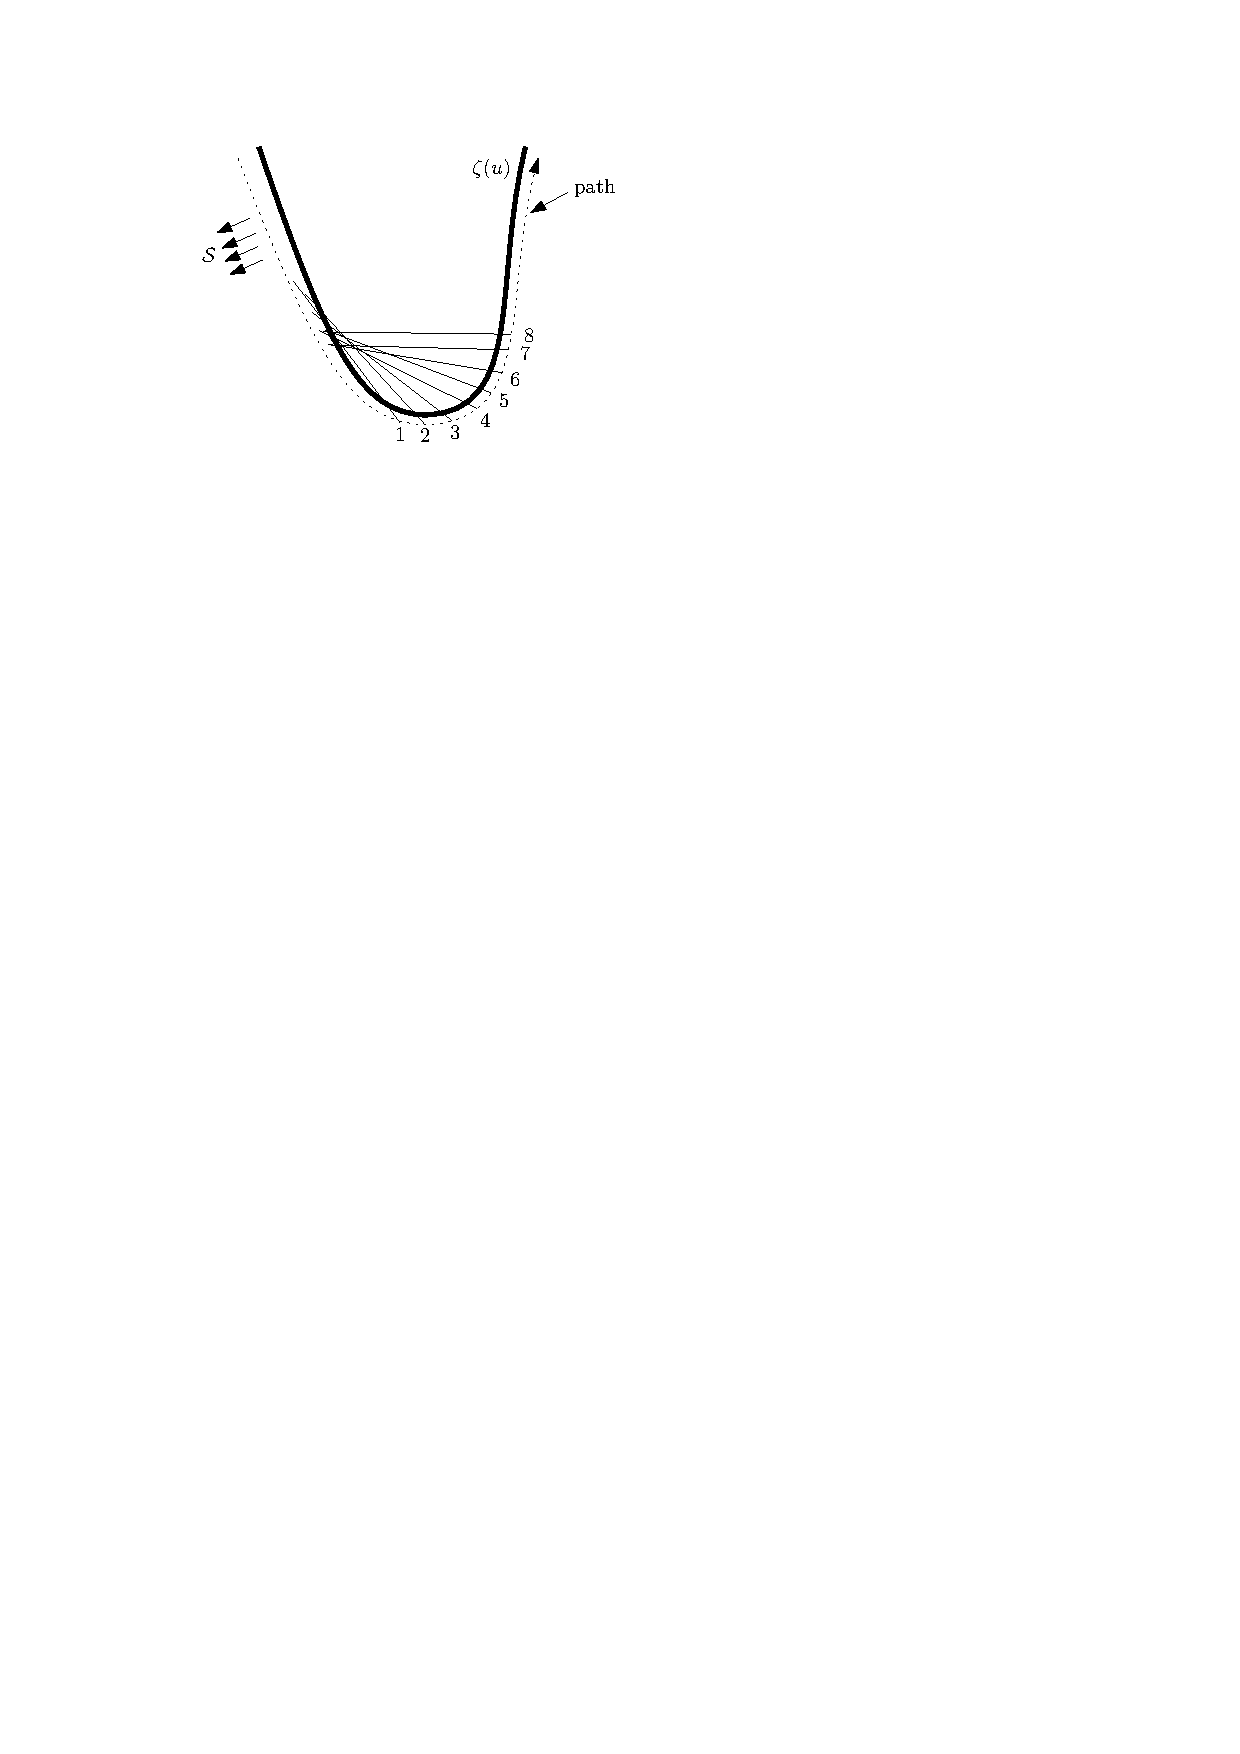
\includegraphics[width=1.15\linewidth]{figures/Traversabilityproblem.pdf}
		\caption{Infeasible link length\label{fig:not_traversable}}
	\end{subfigure}%
	\begin{subfigure}{0.31\textwidth}
		\centering
		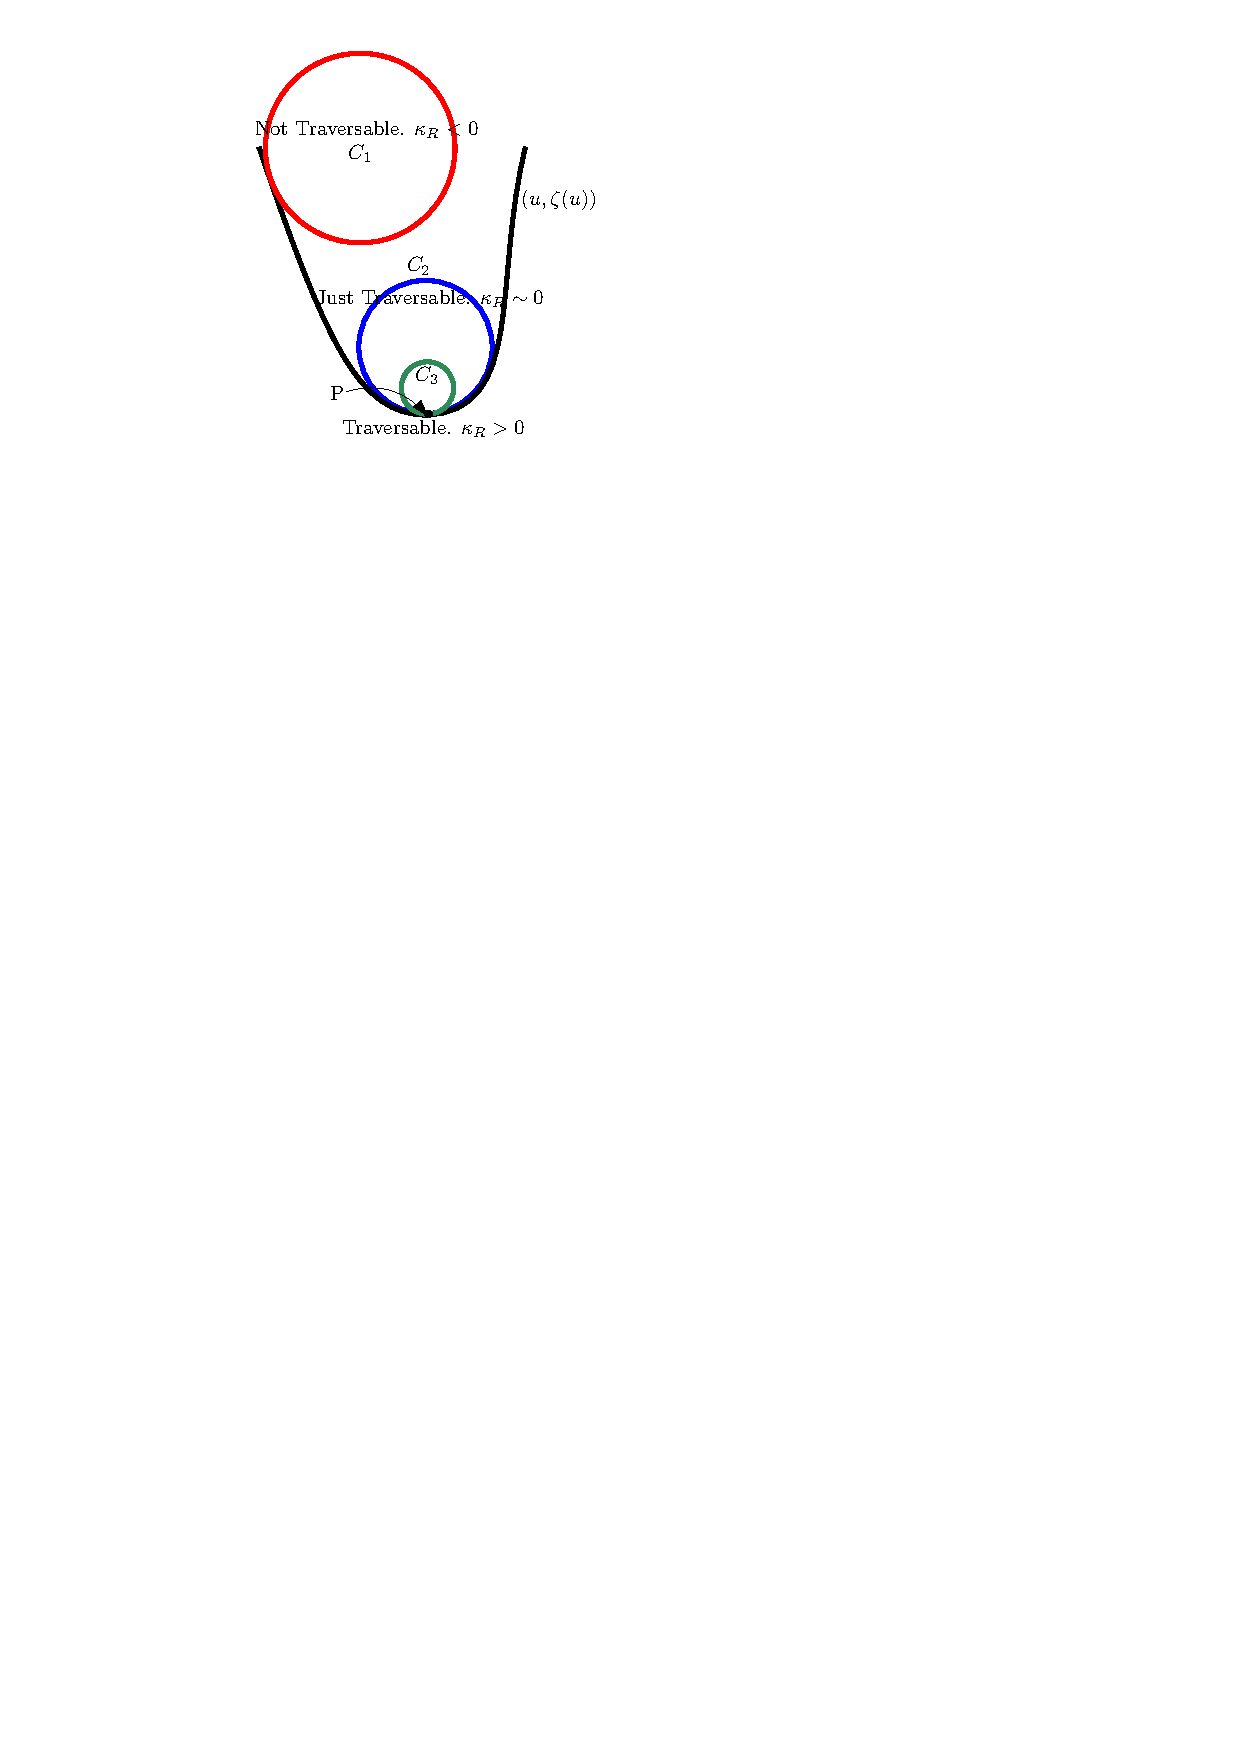
\includegraphics[width=0.75\linewidth]{figures/Traversability.pdf}
		\caption{Traversability of a curve \label{fig:is_traversable}}
	\end{subfigure}%
	\begin{subfigure}{0.31\textwidth}
		\centering
		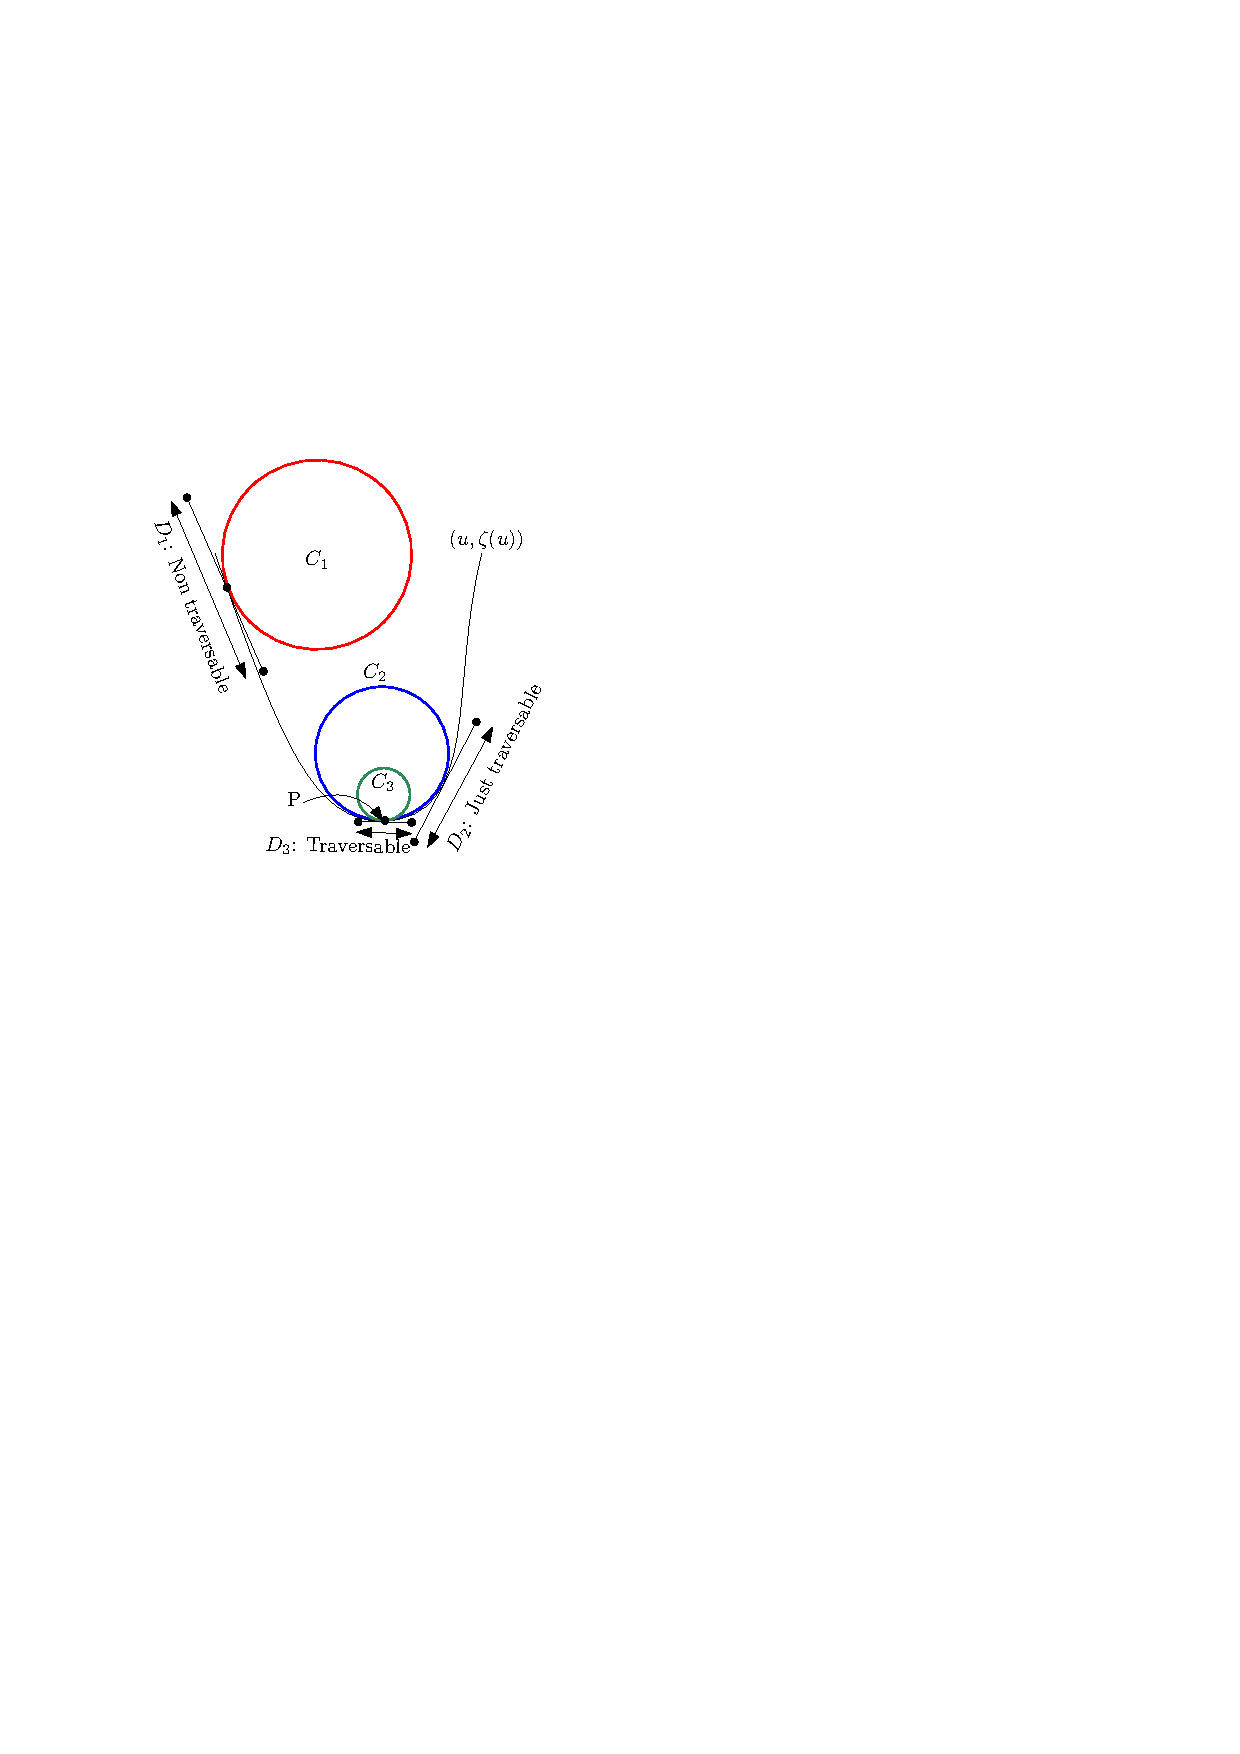
\includegraphics[width=0.85\linewidth]{figures/Traversability2.pdf}
		\caption{Feasible link lengths \label{fig:largest_link}}
	\end{subfigure}
	\caption{ Feasibility of motion planning with a given link length about a given curve.}
\end{figure}
	
%\subsection{Tractrix  emulates natural motion}
%Motion simulated using the approach discussed in this paper imparts realism due to the minimal movement of tail with respect to the head. In nature this effect is created due to the friction or other resistive forces acting in the lateral direction of the link. In the absence of friction, displacement given in the head will result in a simple translation of link. In other words, $\mathbf{x}_t$ in this case, will be same as $\mathbf{x}_h$. In actual practice, there will be a discrepancy between natural movement and the simulation based on the tractrix approach because tractrix represents the ideal scenario with motion of tail limited only in the direction of motion of the link due to very high friction while in natural motion, there is always some degree of translation possible. This slippage could be included in the formulation, however, by adding a slip vector to the tail displacement. Since the slippage amounts to the translation of link in the direction of link, slip vector will be in the direction of head displacement and can be written as as $\mathbf{s} = \nu \mathbf{X}_h$, where $\nu<1$ is a constant. $\nu=0$ represents the ideal tractrix case with friction and $\nu=1$ represents pure translation of the link. Including this vector, the minimization function may be written as:
%\begin{align}
%\min_{\textbf{x}_t} &\Vert \textbf{x}_t-\left(\mathbf{X}_t + \nu \mathbf{X}_h \right) \Vert
%\end{align}
%
%Figure \cref{fig:tractrixemulation} shows the final pose of a bicycle chain pulled from an initial horizontal position along the negative Y-axis on two surfaces: a smooth paper and a rough surface paved with gravel. Using a constant value of $\nu = 0.95$ for paper and $\nu =0.86$ for gravel, we can see from that the formulation conforms with the actual final pose very well. 
%
%\begin{figure}[ht!]
%    \centering
%    \begin{subfigure}{0.48\textwidth}
%        \centering
%        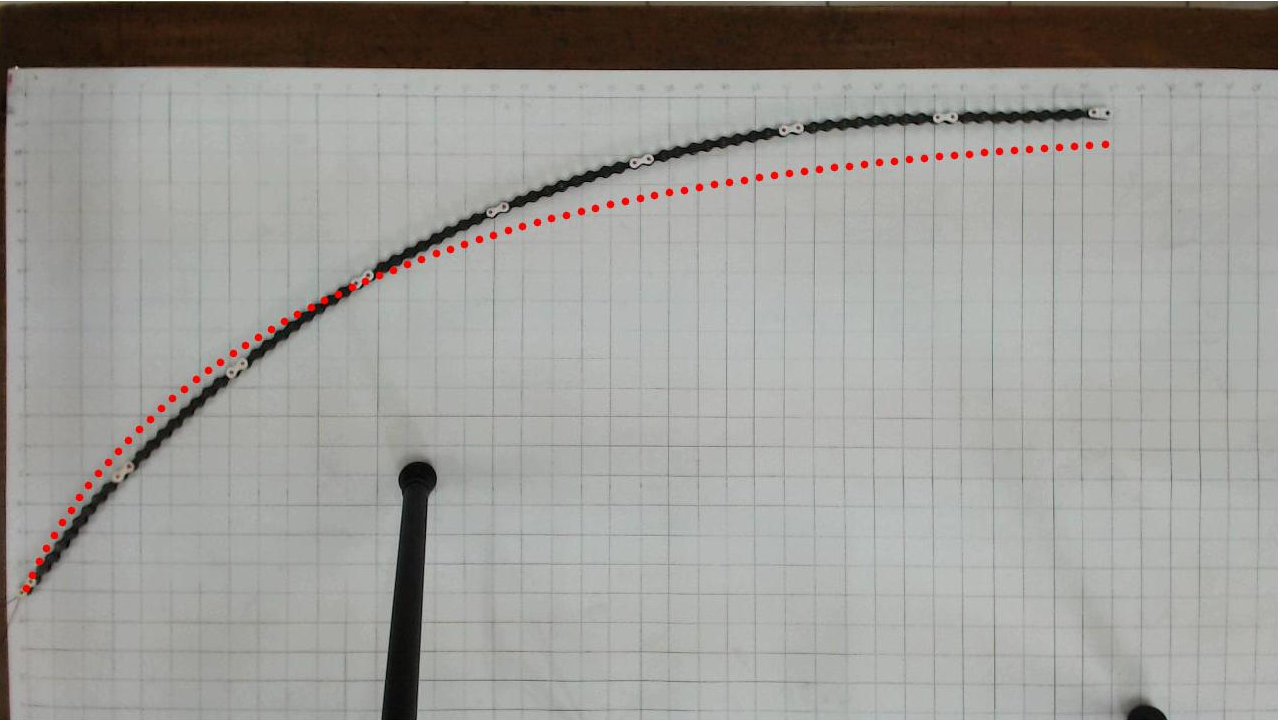
\includegraphics[width=1\linewidth]{figures/figslipa.png}
%        \caption{Tractrix emulating the motion of a bicycle chain on photo paper, $\nu=0.95$}
%   
%    \end{subfigure}%
%    ~
%        \begin{subfigure}{0.48\textwidth}
%        \centering
%        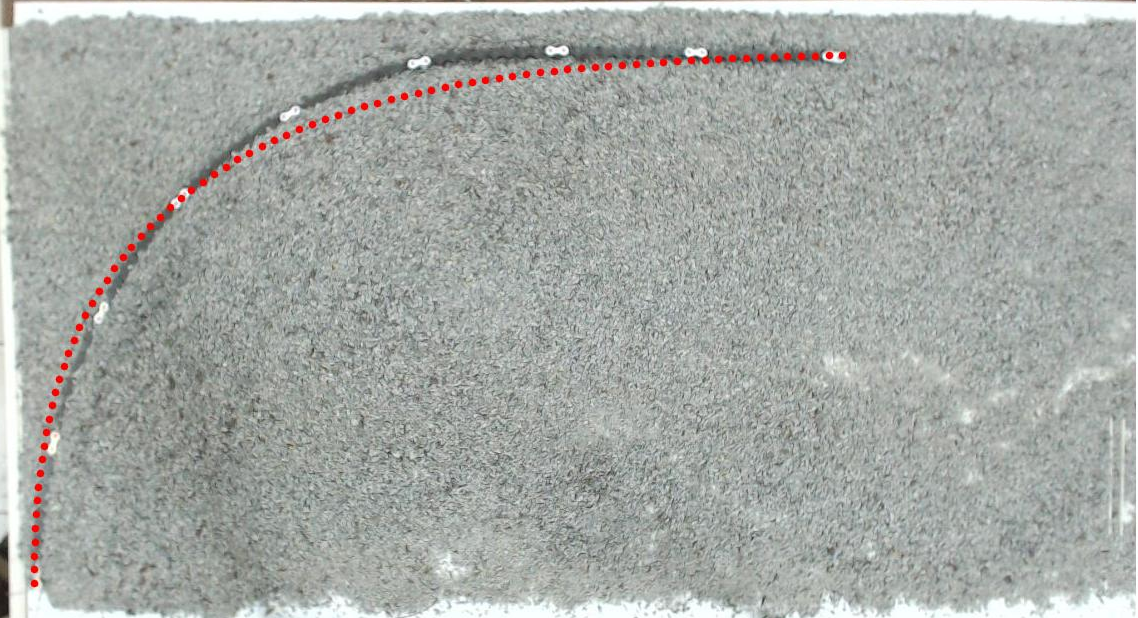
\includegraphics[width=1\linewidth]{figures/figslipb.png}
%        \caption{Tractrix emulating the motion of a bicycle chain on gravel, $\nu=0.86$}
%      \end{subfigure}
%    \caption{ Tractrix with slip emulates natural motion \label{fig:tractrixemulation}}
%\end{figure}

\section{Conclusions}
\label{sec:conclusions}

Motion planning for hyper-redundant robots in narrow ducts using tractrix based redundancy resolution scheme is addressed. To this end, we discussed three methods to represent ducts in 2D plane as a combination of ellipses, as a series of connected quadrilaterals as well as a bound planar surface formed from two non-intersecting analytical curves. Methods to formulate inequality constraints which will impose the tail point of a link to always lie inside the duct are investigated for all the cases. In 3D, representation of ducts as series of ellipsoids, series of connected cylinders and using point clouds is discussed. The basic formulation as well as formulation for efficient practical implementation is discussed. The methods discussed are demonstrated using three practical examples of motion planning of 1) a hyper-redundant inspection robot through an industrial pipeline 2) a highly articulated endoscopic robot through a GI tract and 3) a hyper-redundant robot in search and rescue operation. From the examples, it is shown that the methods discussed in the paper can be effectively used in motion planning of a hyper-redundant robot manoeuvring in confined bounded spaces while emulating realism. Computational complexity for the methods discussed in this paper is analysed. The complexity of the methods scale linearly for the number of links as well as the number of path points for a given problem, while it scales with the order of maximum of 1.5 for the number of constraint equations. The locking condition for links in negotiating ducts of very low radius of curvature is discussed. A maximum link length which could overcome the issue, based on the curvature of the duct walls is suggested.

??uses LAPACK and heavy solvers.. not really required. instead a stripped version of the interior point will do quite well for fast near real-time implementation. ?? Research on algorithms to overcome the locking problem while maintaining motion realism is underway.




\section{Appendix}	\crefalias{section}{appsec}
\subsection{Analytical expressions for $u,v$ for quadrilateral patch}\label{app:Analylit_u_v_quad}
\begin{align}
&\quad {v} = \frac{k_1-k_2\pm \sqrt{\left(k_2-k_1\right)^2-4k_3k_4}}{2k_3},~~{u} = \frac{\left(x-{}^xP_{i-1}+{v}\right)}{\left( a_2+{v} a_3 \right)}\\
\nonumber\text{ where, }k_1 &= \left(b_1b_2+b_0b_3 \right),~~k_2 = \left(a_1a_2+a_0a_3 \right),~~
k_3 = \left(a_1a_3-b_1b_3 \right),~~k_4=\left(a_0a_2-b_0b_2 \right)\\
\nonumber a_0 &= y-{}^yP_{i-1},~a_1 = {}^yP_{i-1}-{}^yP_i,~a_2 = {}^xQ_{i-1}-{}^xP_{i-1},~a_3 = \left({}^xQ_{i}-{}^xP_i\right)-\left({}^xQ_{i-1}-{}^xP_{i-1}\right)\\
\nonumber b_0 &= x-{}^xP_{i-1},~b_1 = {}^xP_{i-1}-{}^xP_i,~b_2 = {}^yQ_{i-1}-{}^yP_{i-1},~b_3 = \left({}^yQ_{i}-{}^yP_i\right)-\left({}^yQ_{i-1}-{}^yP_{i-1}\right)
\end{align}

If ${}^xP_{i-1}={}^xP_{i}$ and ${}^xQ_{i-1}={}^xQ_{i}$, 
\begin{align}
{u} = \frac{b_0}{a_2},~~{v} = \frac{a_0a_2-\left(a_3+a_2 \right)}{a_1\left(b_0-a_2\right)+b_0\left(b_3-b_2 \right)}
\end{align}

\subsection{Parametric equation of solid cylinder}\label{app:parametric_u_v_solid_cyl}
\begin{figure}[ht!]
    \centering
    \begin{subfigure}{0.48\textwidth}
        \centering
        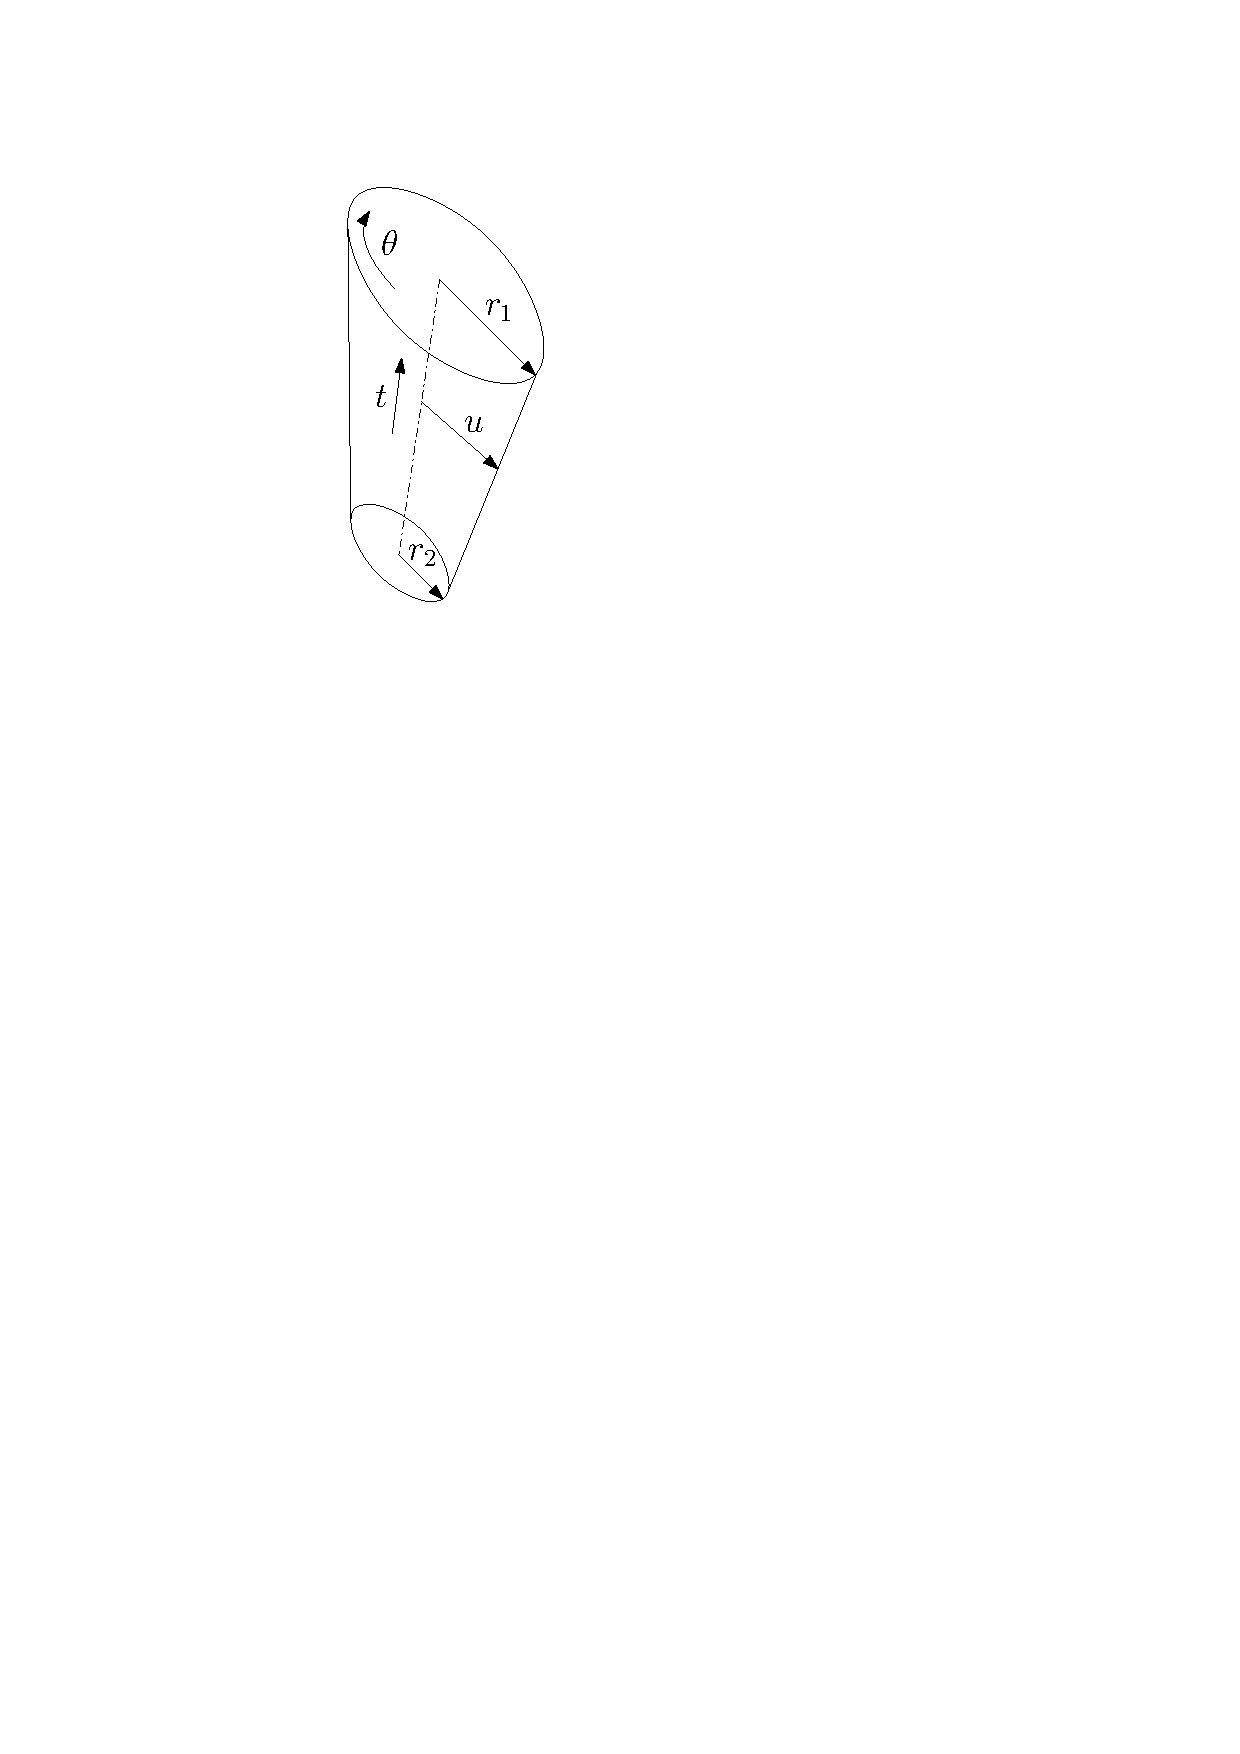
\includegraphics[width=0.3\linewidth]{figures/fig17a.pdf}
        \caption{Parameters of a general cylinder \label{fig:cylparams}}
    \end{subfigure}%
    \begin{subfigure}{0.48\textwidth}
        \centering
        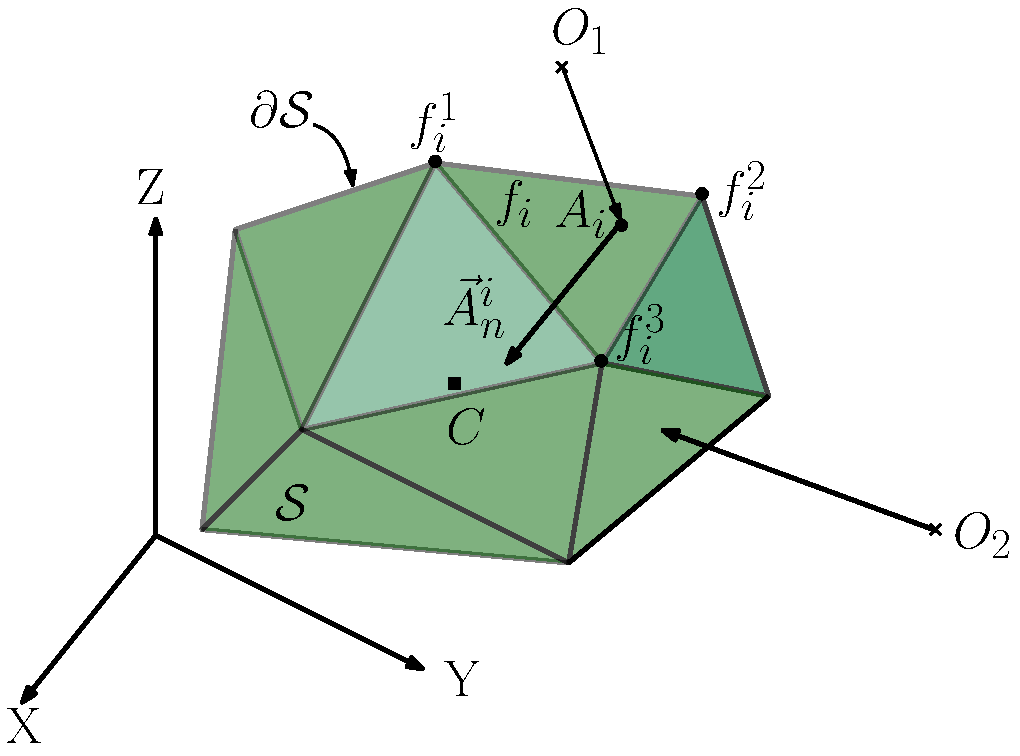
\includegraphics[width=0.85\linewidth]{figures/app_fig1.pdf}
        \caption{Schematic of \cref{alg:in_hull} \label{fig:alg_schematic}}
    \end{subfigure}
\caption{}
\end{figure}
The parametric cylinder, as shown in \cref{fig:cylparams}, with the parameters $u,~\theta$ and $t$ is given as:
\begin{align}
x & = C_1(u,t,\theta)=\left(r_1m_1u\cos\theta +m_2 \right)\left(1-t \right)+\left(r_2n_1u\cos\theta+n_2 \right)t\\
y & = C_2(u,t,\theta)=\left(r_1m_3u\cos\theta +r_1m_4u\sin\theta +m_5 \right)\left(1-t \right)+\left(r_2n_3u\cos\theta+r_2n_4u\sin\theta+n_5 \right)t\\
z & = C_3(u,t,\theta)=\left(r_1m_6u\cos\theta +r_1m_7u\sin\theta +m_8 \right)\left(1-t \right)+\left(r_2n_6u\cos\theta+r_2n_7u\sin\theta+n_8 \right)t
\end{align}
where
\begin{align*}
&m_1= \cos{}^1\phi_2,~m_2 = {}^1x_c,~&m_3 = \sin{}^1\phi_1\sin{}^1\phi_2,~m_4=\cos{}^1\phi_1, \nonumber \\
&m_5 = {}^1y_c,~m_6=-\cos{}^1\phi_1\sin{}^1\phi_2,~&m_7=\sin{}^1\phi_1,~m_8={}^1z_c \nonumber\\
&n_1 = \cos{}^2\phi_2,~n_2 = {}^2x_c,~&n_3 = \sin{}^2\phi_1\sin{}^2\phi_2,~n_4=\cos{}^2\phi_1, \nonumber \\
&n_5 = {}^2y_c,~n_6=-\cos{}^2\phi_1\sin{}^2\phi_2,~&n_7=\sin{}^2\phi_1,~n_8={}^2z_c \nonumber
\end{align*}
The quantity ${}^1\left(\cdot\right)$ and ${}^2\left(\cdot\right)$ represent the corresponding parameters of the circles at the ends of the cylinder. $\phi_1$ and $\phi_2$ are the angles about the Y and X-axes which the plane of the circle is rotated, $(x_c,y_c,z_c)$ is the co-ordinate of the center of the circle.

\subsection{An algorithm for classifying a point with respect to a polyhedron}\label{app:polyhedron_point}
\indent Classification a point with respect to a triangulated domain is a very well known problem and many methods exist, which offer various advantages in terms of computational complexities. In \cref{alg:in_hull}, we describe a method, to classify a given set of points $O$ with respect to a polyhedron $\mathcal{P}$ as inside ($O_{in}$) and outside ($O_{out}$). The implementation of our algorithm\footnote{We have used a modified version of the Matlab function inhull.m, made available by John D'Errico for free usage. } is $\mathcal{O}(m)$. The algorithm can be visualized from \cref{fig:alg_schematic}.
\begin{algorithm}[ht!]
	\textbf{Purpose :} To classify a set of points $ O $ with respect to  boundary $\partial \mathcal{P}$\\
	\KwIn{The set $ O $, $O\in \Re^3$ and $O \equiv O_{in}\cup O_{out}$ }
	\KwOut{$ O_{in},~ O_{out}$}
	\begin{algorithmic}[1]
		\STATE Obtain $C$, the center of $\mathcal{P}$ by taking the mean of the vertices of the $N$ facets constituting $\partial \mathcal{P}$
		\FOR {$i=1,2,...,N$}
		\STATE Calculate the normal to the $i^{th}$ facet, $A_n^i=(f_i^1-f_i^2)\times(f_i^2-f_i^3)$
		\STATE Choose a point $A^i$ on the $i^{th}$ facet and move $A_n^i$ to $A^i$
		\STATE Ensure that $A_n^i$ is directed inside, towards $C$
		\STATE $H(i)=\langle\vec{O_i-A_i}, A_n^i\rangle$
		\ENDFOR 
		\IF {$H(i)\geq 0 ~\forall i$}
		\STATE Classify $O_1 \in O_{in}$ as inside, otherwise classify $O_1\in O_{out}$  		
		\ENDIF
	\end{algorithmic}
	
	\caption{Algorithm for classifying points as inside ($O_{in}$) or outside ($O_{out}$) of a triangulated domain. }		
	\label{alg:in_hull}
\end{algorithm}

%\bibliography{journalref}


\begin{thebibliography}{99}

We have to see IEEE reference format.
%%1
%\bibitem{Gaylord1958}
%R.~H. Gaylord (1958), 
%\newblock ``Fluid actuated motor system and stroking device'',
%\newblock {\em US Patent  2,844,126} (July~22 1958).
%
%%2
%\bibitem{Joseph1960}
%L.~Joseph (1960), 
%newblock ``Artificial muscle'', 
%\newblock {\em Life} {\bf 14}, pp. 87--88.
%
%%3
%\bibitem{Pillsbury2015}
%T.~E. Pillsbury, C.~S. Kothera, N.~M. Wereley (2015),
%\newblock `` Effect of bladder wall thickness  on miniature pneumatic artificial muscle performance'', 
%\newblock{\em Bioinspiration \& Biomimetics}, {\bf 10}~(5), pp. 055006.


\end{thebibliography}


\end{document}
